% ============================================================
% Projective Dynamic Logo (PDL)
% Global Mapping of Structures, Results, and Open Problems
% Version 34 — C. Laubscher % Supersedes DM v33 (10.5281/zenodo.21520303)
% ============================================================
\documentclass[11pt,a4paper]{article}

% ---- Encoding and fonts ----
\usepackage[utf8]{inputenc}
\usepackage[T1]{fontenc}
\usepackage{lmodern}
\usepackage{newtxtext}

% ---- Page layout ----
\usepackage[margin=2.5cm]{geometry}

% ---- Mathematics ----
\usepackage{amsmath,amssymb,amsthm}
\newtheorem{resolvedproblem}{Resolved Problem}
\newcommand{\Rval}{R_{\mathrm{val}}}
\newcommand{\Rsea}{R_{\mathrm{sea}}}
\newcommand{\Rres}{R_{\mathrm{res}}}

% ---- Tables and lists ----
\usepackage{booktabs}
\usepackage{longtable}
\usepackage{array}
\usepackage{ragged2e}
\usepackage{enumitem}
\newcommand{\hb}{\hbar}
\newcommand{\Cspin}{{\mathcal{C}_{\mathrm{spin}}}}
\newcommand{\Cmass}{{\mathcal{C}_{\mathrm{mass}}}}
\newcolumntype{L}[1]{>{\RaggedRight\arraybackslash}p{#1}}

% ---- Graphics ----
\usepackage{graphicx}
\usepackage{float}
\usepackage{tikz}
\usetikzlibrary{positioning,backgrounds,arrows.meta,fit}
\pgfdeclarelayer{background}
\pgfsetlayers{background,main}

% ---- Captions and colours ----
\usepackage[font=small,labelfont=bf]{caption}
\captionsetup[table]{labelsep=quad}
\usepackage{xcolor}
\definecolor{proofblue}{RGB}{0,70,140}
\definecolor{conjecturegreen}{RGB}{0,120,60}
\definecolor{hypothesisorange}{RGB}{200,90,0}
\definecolor{openproblemred}{RGB}{170,0,0}
\definecolor{negativered}{RGB}{160,20,20}

% ---- Hyperlinks ----
\usepackage{hyperref}
\usepackage{doi}
\usepackage{url}
\hypersetup{
colorlinks=true,
linkcolor=proofblue,
citecolor=proofblue,
urlcolor=proofblue}

% ---- Bibliography ----
\usepackage[numbers,sort&compress]{natbib}

% ---- Theorem environments ----
\theoremstyle{plain}
\newtheorem{theorem}{Theorem}[section]
\newtheorem{proposition}[theorem]{Proposition}
\newtheorem{corollary}[theorem]{Corollary}
\newtheorem{lemma}[theorem]{Lemma}
\theoremstyle{definition}
\newtheorem{definition}[theorem]{Definition}
\newtheorem{axiom}[theorem]{Axiom}
\theoremstyle{remark}
\newtheorem{remark}[theorem]{Remark}
\newtheorem{conjecture}[theorem]{Conjecture}
\newtheorem{openproblem}[theorem]{Open Problem}
\newtheorem{namedhyp}[theorem]{Named Hypothesis}
\newtheorem{hypothesis}[theorem]{Hypothesis}

% ---- Custom macros ----
\newcommand{\PDL}{\textnormal{PDL}}
\newcommand{\Kfour}{K_4}
\newcommand{\quintuplet}{(24,\,28,\,930,\,10087,\,11017)}
\newcommand{\Geff}{G_{\mathrm{eff}}}
\newcommand{\GPDL}{G_{\mathrm{PDL}}}
\newcommand{\epsG}{\varepsilon_G}
\newcommand{\rval}{r_{\mathrm{val}}}
\newcommand{\Rsurf}{R_{\mathrm{surf}}}
\newcommand{\Rtot}{R_{\mathrm{tot}}}
\newcommand{\sigmaN}{\sigma(N)}
\newcommand{\mustar}{\mu^*}
\newcommand{\SBH}{S_{\mathrm{BH}}}
\newcommand{\Meff}{M_{\mathrm{eff}}}
\newcommand{\MPl}{M_{\mathrm{Pl}}}
\newcommand{\Tpp}{T_{pp}}
\newcommand{\Zsat}{Z_{\mathrm{sat}}}
\newcommand{\rexc}{r_{\mathrm{exc}}}
\newcommand{\Nmin}{N_{\min}}
\newcommand{\epsGeomB}{\varepsilon_G^B}
\newcommand{\rhocoh}{\rho_{\mathrm{coh}}}
\newcommand{\Ccoh}{C_{\mathrm{coh}}}
\newcommand{\VC}{V_C}

\newcommand{\Vfour}{V_4}
\newcommand{\Sfour}{S_4}
\newcommand{\Sthree}{S_3}
\newcommand{\Ggauge}{G_{\mathrm{gauge}}}
\newcommand{\Uone}{\mathrm{U}(1)}
\newcommand{\SUtwo}{\mathrm{SU}(2)}
\newcommand{\SUthree}{\mathrm{SU}(3)}
\newcommand{\Coh}{\mathrm{Coh}(K_4)}
\newcommand{\Dmu}{D_\mu}

% ---- List style ----
\setlist[itemize,1]{label=\textendash}
\setlist[itemize,2]{label=\textbullet}

% ============================================================
\title{Projective Dynamic Logo (PDL)\\[4pt]
\large Global Mapping of Structures, Results, and Open Problems\\[2pt]
\normalsize Version 34 --- A Guide for Continuation of the Programme}
\author{C\'edric Laubscher\\[4pt]
\small Independent researcher\\
\small \href{https://cedriclaubscher.ch}{cedriclaubscher.ch}
$\;\cdot\;$
\small \href{https://zenodo.org/communities/pdl-framework/}{zenodo.org/communities/pdl-framework}}
\date{\today}

\begin{document}

\maketitle
\setcounter{tocdepth}{2}

% ============================================================
\begin{abstract}
This document provides a systematic and self-contained guide to the Projective Dynamic Logo (PDL) programme, intended for a scientific colleague who wishes to understand, verify, or continue the research. PDL is a foundational physics programme that derives fundamental physical constants and dynamical laws from four axioms on finite signed graphs, without presupposing spacetime, particles, or fields. The minimal admissible closure under the axioms is the complete signed graph $\Kfour$ on four vertices and six edges, identified with the electron prototype. The proton is characterised by a unique integer quintuplet $\quintuplet$, from which all results flow.

The current corpus (D01--D69, plus auxiliary documents, the PDL-V series DL01--DL03, and the joint PDL--OFN bridge notes N01 and N02) has reached the following state:
\begin{itemize}
\item Three critical Gates have been resolved: the axiomatic derivation of the amplitude $155/11017$ (Gate~1, D29), the structural proof that the QCD correction coefficient equals~2 (Gate~2, D30), and the theorem $\Geff(N)=\sigmaN\cdot\GPDL$ (Gate~3, D31/D36).
\item The quantum dynamics layer is \textbf{complete}: the Schr\"odinger equation (D32), Dirac equation (D33), Born's rule Level~1 via Gleason uniqueness (D34), the Einstein coupling equation (D35), Born's rule Level~2 including $\mathrm{U}(1)$ phase freedom (D46), and the London equation (D49) have all been derived from C1--C4 with no free parameter.
\item Newton's gravitational constant $G$ is derived from the axioms modulo a single irreducible external parameter ($\Delta m_{\mathrm{iso}} = m_d - m_u$) \textbf{and, as established in v34, one named structural hypothesis} (H$\varphi$, Section~\ref{sec:Hphi}). It is a theorem \emph{under} H$\varphi$, not an unconditional theorem. \textcolor{negativered}{In addition, OP-B is reopened by D44v2: the filter factor $k$ is no longer a proved consequence of C1--C4 (Section~\ref{sec:numerical}).} No adjustable parameter is introduced by either correction.
\item The Hubble tension is resolved at $0.006\%$ with zero free parameters (D35/D27).
\item Black hole thermodynamics is \textbf{complete}: the area law $S \propto \Rsurf$ (D37), the Bekenstein--Hawking formula $\SBH/k_B = 4\pi(\Meff/\MPl)^2$ (D38), the one-quarter coefficient $\tfrac{1}{4}$ in $\SBH = k_B A/(4\ell_P^2)$ (D50), and the London equation (D49) are all unconditional theorems.
\item Open Problem~OP1 has been fully resolved by D42: the Indifference Lemma~H3 is now an unconditional theorem of axioms~C1--C4.
\item D46 resolves OP4: the $\mathrm{U}(1)$ phase freedom of quantum mechanics is derived from the $\Kfour$ pulsation structure, completing the quantum dynamics layer.
\item D47v1 claimed to resolve OP13 and OP14: the spin--orbit splitting $\Delta n = 4$ is forced by a unique perfect-square discriminant ($149^2$), the Mirror Lemma establishes proton--neutron HO-PDL level isomorphism, and (as originally claimed) the sub-shell filling rates $r_{\mathrm{exc}}(Z)$ were derived analytically for all $Z = 1$--82. \textcolor{negativered}{An independent audit (Session~74, reported in D47v2) shows the OP14 claim does not survive confrontation with D40's own filling-rate table under the correct reconstruction formula: the two-valued rule of D47v1 reproduces 0 of 31 experimental sub-shell boundaries, and a textual remark in D47v1 mischaracterising D40's table is factually incorrect.} OP13 and the Mirror Lemma are unaffected and independently re-verified. \textbf{OP14 is reopened}; the nuclear stability layer is complete for OP13 and the magic numbers only.
\item D48v3 fully resolves OP2-D35 and OP-spin: the coherence stress-energy tensor $\Ccoh$ is derived with four unconditional components. $C^{(\mathrm{mass})}$ and $C^{(\mathrm{orb})}$ are unconditional theorems; $C^{(\mathrm{spin})}=0$ in the homogeneous ground state (theorem from explicit computation over all 8 coherent configurations of $K_4$, resolving OP-spin); $C^{(\mathrm{leak})}$ is a theorem via D51+D52 in dimensionally consistent units J\,m$^{-3}$. Four dimensional errors from v1/v2 are corrected.
\item D49 resolves OP-London: the London equation $j^i_s = -(n_{\mathrm{coh}} e^2/m_p c) A^i$ is derived from C1--C4 via the metric identity $\nu = \tfrac{1}{4}\|\psi_1 - T^k\psi_1\|^2$ (768/768 exhaustive verification) and axiom~C4.
\item D50 resolves OP12/BH-3: the coefficient $\tfrac{1}{4}$ in the Bekenstein--Hawking formula is derived from C1--C4 as the stable fraction $4/16$ per surface relation, under H3 (D42).
\item D51 and D52 together resolve OP1-D35: the cosmological leakage constant is $C = (1-\kappa)^{997} \times (930/11017)^{23} \times (1-\eta_L)^{67}$, agreeing with the observational bound to 0.17~ppm. The causal chain $\mathrm{C1}\text{--}\mathrm{C4} \to \Kfour \to \beta_1=3 \to (p_{k_1},p_{k_2},p_{k_3}) \to C \to \Lambda_{\mathrm{PDL}}$ is complete.
\item D53 provides a self-contained synthesis of the complete causal chain C1--C4 $\to$ $\Lambda_{\mathrm{PDL}}$, with an independent numerical verification of $C_{\mathrm{PDL}}$ to $0.41$~ppm relative to D51, and a systematic robustness analysis of the prime exponent structure. The chain spans fifty-seven orders of magnitude from combinatorial axioms to the cosmological constant.
\item D40 derives the complete architecture of nuclear stability from the proton and neutron quintuplets alone: $\Nmin(Z) = Z$ for $Z \leq 20$ as an exact theorem, the conflict saturation $C(Z>20) = 190\,\Tpp$ exactly, and the valley of stability reproduced at $100\%$ accuracy for all $Z=1$ to $82$.
\item D41 confronts the PDL framework with the experimental results of Ha et al.\ (\textit{Nature Communications} 16, 10631, 2025), confirming the structural identity $T \approx (\Delta n+1)^2 = 25$ across three independent observables, with the wave-function component ratio agreeing at the $2\%$ level.
\item D43 establishes the computational infrastructure of the programme and proves the geometric leakage parameter $\varepsilon_{\mathrm{geom}}(p) = 329/10087$ as an unconditional theorem (OP-A resolved).
\item D44 derives the hierarchical filter factor $k = 0.921716$ from C1--C4 as an unconditional theorem (OP-B resolved). The complete causal chain C1--C4 $\to$ $K_4$ $\to$ quintuplet $\to$ $\varepsilon_{\mathrm{geom}}$ $\to$ $\varepsilon_G = \varepsilon_{\mathrm{geom}} \times k^{18}$ $\to$ $G$ is now fully closed with no remaining open problem and no free parameter beyond $\Delta m_{\mathrm{iso}}$.
\item D45 derives the first falsifiable astrophysical confrontation: the primordial black hole survival threshold is shifted upward by $+11.89\%$ relative to the standard GR value, giving $M^*_{\mathrm{PDL}} = \sigma(40)^{-2/3}\,M^*_{\mathrm{GR}} \approx 5.706 \times 10^{14}$\,g, testable with existing Fermi-LAT data via \textsc{BlackHawk} and \textsc{Isatis}.
\item \textbf{New in v22 --- D54} resolves OP-pressure~\cite{D54}: the equation of state of the PDL coherence fluid is $w(N) = -\rho_\Lambda/\rhocoh(N)$, an unconditional theorem of C1--C4. In the homogeneous ground state, $w_{\mathrm{mass}} = w_{\mathrm{spin}} = w_{\mathrm{orb}} = 0$ exactly (three distinct theorems), and $w_{\mathrm{leak}} = -1$ intrinsically. The PDL dark-energy fraction $\Omega_\Lambda^{\mathrm{PDL}} = \rho_\Lambda/\rho_{\mathrm{crit}} = 0.6838$ agrees with the Planck~2020 value $\Omega_\Lambda^{\mathrm{obs}} = 0.685$ to $0.17\%$, with no cosmological parameter as input. The PDL coherence fluid interpolates between pressureless cold matter at sub-nuclear scales and dark energy at cosmological scales --- both emerging from the same combinatorial structure with no parameter adjustment.
\item \textbf{New in v23 --- D55} resolves OP10 at the level of the Weinberg angle~\cite{D55}: the formula $\theta_W = 19\pi/119$ is derived as an unconditional theorem of C1--C4, via four established results (D33, D46, D51, and the new Lemma~D) and zero free parameters. The key structural result is that $\theta_W$ is a dephasing sequencing ratio: the Berry phase accumulated during $k_2 = 19$ elementary interface steps out of $N_{\mathrm{total}} = 119$, where $k_2 = n_u - R_e + 1$ (D51 theorem) and $N_{\mathrm{total}} = (n_d/4)\cdot(r_d-r_u)/R_e = 7\times 17$ (Lemma~D, proved exhaustively over all 768 $(A)\wedge(B)$ configurations). The predicted $\sin^2\theta_W = 0.231196$ agrees with the PDG~2024 value $0.23121\pm0.00003$ at $0.48\,\sigma$. As a secondary result, combining with the geometric zeroth-order formula yields a new PDL prediction $\Delta m_{\mathrm{iso}} = 2.446$~MeV (within $0.92\,\sigma$ of FLAG~2024), falsifiable by next-generation lattice QCD. The electroweak sector of the Standard Model is now structurally derived from C1--C4.
\item \textbf{New in v24 --- D56} resolves OP-D41-1-A~\cite{D56}: the number of maximal partial closures on a $k$p-$k$h nuclear interface surface is $N_{\mathrm{comp}}(k)=k$ exactly, proved from three lemmas (uniqueness on one unit, disjointness of mixed-triangle sets, C3-irreducibility of the assembly) and verified for $k=1,\ldots,5$.
\item \textbf{New in v28 --- D61} resolves OP-D59-2~\cite{D61}: the minimal covariant derivative $D_\mu = \partial_\mu - igA_\mu$ is derived from C4 as a survival theorem. The group of C4-admissible discrete transports on $K_4$ is $\mathrm{Coh}(K_4) \cong \mathbb{Z}_2^3$ (2048 exhaustive checks); $V_4$ acts faithfully on this group by automorphisms with fixed-point subgroup $F \cong V_4$ labelled by the three perfect matchings of $K_4$ (288 checks); the equivariant connected completion is $G_\mathrm{gauge} = \mathrm{SU}(3)\times\mathrm{SU}(2)\times\mathrm{U}(1)$, consistent with D46--D60; and Utiyama's uniqueness theorem identifies $D_\mu$ as the unique first-order equivariant generator. The gauge sector of the Standard Model --- group, representations, and gauge dynamics --- is now completely derived from C1--C4, without variational postulate and without free parameter at the structural level.
\item \textbf{New in v28 --- D60}~\cite{D60} proves Hypothesis H$_{\mathrm{SU2}}$ as an unconditional theorem of C1 and C2 alone (OP-D57-1 resolved). The $V_4$-invariance of the pulsation structure forces $G_{\mathrm{eff}} = S_4/V_4 \cong S_3$, establishing the complete logical chain from the axiom of existence (C1) to the effective gauge symmetry group, with no conjectural step remaining in the gauge sector.
\item \textbf{New in v25 --- D57}~\cite{D57} provides the first combinatorial derivation of the tree-level Weinberg angle from C1--C4 alone: $\sin^2\theta_W^{(\mathrm{tree})} = \sin^2(\pi/R_e) = 1/4$, where $R_e = 6$ is the relational budget of $\Kfour$ (number of edges), itself a theorem of C1--C4 (D16a). Two independent routes are proved equivalent: the combinatorial route ($192/768 = 1/4$ from the $(A)\wedge(B)$ criterion, D29) and the orbit route ($\dim(\mathbf{1})/\dim(\text{orbit-4}) = 1/4$ from the $S_4$ action on coherent configurations). Both routes identify the factor $1/4$ with $|V_4|/16$. The quotient $A_4/V_4 \cong \mathbb{Z}_3$ is identified as the combinatorial origin of $\beta_1(K_4) = 3$, providing a partial resolution of OP-OFN-1 (N01~\cite{N01}).
\item \textbf{New in v25 --- N01} (Laubscher \& Evdokimov) establishes the PDL--OFN bridge~\cite{N01}: $\beta_1(\Kfour)=3$ and $b_1(\Omega_{21})=3$ under Hamming distance-1 adjacency are the same topological invariant viewed from two independent frameworks. Five Python scripts verified the convergence exhaustively. Open Problem OP-OFN-1 (formal derivation of the link between the three PDL leakage cycles and the three OFN fermion generations) is identified; partial resolution provided by $A_4/V_4 \cong \mathbb{Z}_3$ (D57).
\item \textbf{New in v22 --- PDL-V programme (DL series):} Documents DL01~\cite{DL01} and DL02~\cite{DL02} inaugurate a structurally distinct extension of the PDL framework to the threshold conditions for life and consciousness. DL01 introduces the self-replication operator $S$ and establishes that $S(K_4) \cong K_4$ (8/8 coherent configurations), that $\delta^* = 1/2$ is an invariant, and that the rarity law $f(n) = 2^{n+1-\binom{n}{2}}$ holds exactly. DL02 proves three analytical theorems: $K_4$ is the unique fixed point of $S$ (Theorem~1); the life threshold strictly precedes the consciousness threshold, $n^*_{\mathrm{life}} < n^*_{\mathrm{consciousness}}$ (Theorem~2); and both thresholds are finite, $n^*_{\mathrm{max}} < \infty$ (Theorem~3), giving the hierarchy $4 < n^*_{\mathrm{life}} < n^*_{\mathrm{consciousness}} < n^*_{\mathrm{max}} < \infty$ as an unconditional theorem of C1--C4. These documents are presented in Part~III of this mapping, clearly separated from the physical constants programme of Part~I and~II. 
\item \textbf{New in v27 --- D59} constructs the fundamental representation $\mathbf{3}$ of $\mathrm{SU}(3)$ from C1--C4 and identifies the physical colour gauge group $\mathrm{SU}(3)_c$. The carrier space is the trace-zero plane $W = \{(a,b,c)\in\mathbb{C}^3 : a+b+c=0\}$, whose axes are canonically labelled by $V_4\setminus\{e\}$. Five lemmas verified by exhaustive exact-integer computation (\texttt{PDL\_D59\_script1.py}~\cite{D59py}): (L1)~$S_3$-action on $V_4\setminus\{e\}$ faithful and transitive; (L2)~$\chi_\pi = \chi_{\mathrm{trivial}} + \chi_{\mathrm{standard}}$; (L3)~$W = \{a+b+c=0\}$ unique $S_3$-invariant complement of $\mathbb{C}(1,1,1)$; (L4)~$A_2$ root system in $W$, Cartan matrix $\bigl[\begin{smallmatrix}2&-1\\-1&2\end{smallmatrix}\bigr]$; (L5)~isospin asymmetry $\Delta n = n_d - n_u = 4 > 0$ (D47, theorem of C4) selects $\mathbf{3}$ over $\bar{\mathbf{3}}$, identifying the matter sector from the axioms. Exact identity: $k_3/(k_1+k_2) = R_e = 6$. Negative result documented: bijection $(T_2)\leftrightarrow(T_3)$ physically motivated but not $S_4$-equivariant. OP-D58-1 and OP-D58-3 resolved.
\item Gauge boson masses have been partially derived: the ratio $M_Z/M_W = 1/\cos(19\pi/119)$ is an unconditional theorem (D62); the electroweak vev $v = N_{\mathrm{tot}}^2/(R_e k_1)\cdot m_p$ is conjectured at 676~ppm; and the Higgs mass is predicted as $M_H/m_p = 133.611$ at $1.49\,\sigma$ (D62). Five new open problems (OP-D62-1 through OP-D62-5) are identified.
\item The quark mass spectrum has been addressed by two conjectures of distinct ontological character (D63): H\_mass derives $m_d/m_u = 2401/1104$ as the ratio of coherence-pulsation costs of the valence cores $K_{24}$ and $K_{28}$, giving $m_u = 2.155$~MeV and $m_d = 4.687$~MeV within $0.37\%$ of PDG values with no additional free parameter; H\_sea reproduces the sea quark masses $m_s$, $m_c$, $m_b$, $m_t$ within $2.5\%$ of PDG via a residual-fluidity weighting $R_{\mathrm{sea}}/(R_{\mathrm{sea}}+r(n))$. A structural identity $n_u - 1 = p_{k_1} = 23$ connects the hadronic and cosmological sectors for the first time.
\item \textbf{New in v30 --- D64} establishes, for the first time explicitly, a structural correspondence between the surface-degeneracy theorem of D50 ($\Omega_{\mathrm{surf}}=4^{\Rsurf}$ microstates on the proton's active surface at fixed global quantum numbers) and the soft-hair programme of Hawking, Perry and Strominger, in which a black hole carries an infinite-dimensional space of supertranslation and superrotation charges at fixed mass, charge and angular momentum~\cite{D64}. The correspondence is presented as a structural analogy, not a claim of mathematical identity. D64 also reports an honestly negative result: a naive nucleon-counting extrapolation of the PDL per-relation degeneracy fails the Bekenstein--Hawking target by $36.7$ orders of magnitude, a discrepancy proved mass-independent by algebraic construction and verified identically across four black holes spanning eight orders of magnitude in mass (one solar mass, M87*, Sagittarius~A*, GW150914 remnant). Two open problems are introduced: OP-D64-1 (the genuine microstate-counting problem for macroscopic assemblies) and OP-D64-2 (a fully relational unit system deriving $c$ and $\mu^*$ from C1--C4).
\item \textbf{New in v30 --- D65} is a direct sequel to D64, asking whether PDL predicts shared \emph{behaviours} between its two most extreme closures --- the isolated proton and the macroscopic black hole horizon --- independently of any absolute microstate count~\cite{D65}. Five results are established: (1) any closed spherical PDL surface is forced, by a combinatorial analogue of the Poincar\'e--Hopf theorem verified independently by spinor relaxation, exact discrete Gauss--Bonnet computation, and holonomy calculation, to carry exactly two coherence defects, never zero --- a structural, axiom-level account of why no black hole is ever observed with exactly zero spin; (2) the curvature-migration exponent governing the approach to extremality is exactly~$1$, once floating-point noise is eliminated by arbitrary-precision arithmetic, in tension with the third law of black hole thermodynamics, reported openly as OP-D65-2; (3) a dissolution threshold derived from the nucleon saturation number $\Zsat=20$ (D22) gives a critical mass $M^*\approx4.3\,M_\odot$ falling inside the observed compact-object mass gap, an output rather than an input of the construction; (4) seven independent attempts at an absolute microstate count or a Bardeen--Thorne-type spin-limiting mechanism are reported as failures, each with its precise structural cause; (5) these results are organised under the \emph{behaviour-versus-magnitude principle}: PDL currently supports claims about what is topologically forced or what functional form a law must take at the black hole scale, but not yet about absolute magnitude, and this asymmetry is argued to be structural rather than a temporary shortage of derivation effort. Three open problems are introduced (OP-D65-1 through OP-D65-3), the third of which --- constructing the coherence stress-energy tensor and equation of state for an inhomogeneous, symmetry-broken closure rather than the homogeneous limit --- is identified as the single most consequential open problem for future PDL work on black holes.
\item \textbf{New in v30 --- PDL--OFN collaboration, Session~67.} An in-depth exchange with Oleg Evdokimov produced five precise connections between PDL and the Ontological Fundamental Network (OFN), reported here for the first time. (i) The tripartition $\{A,B,C\}$ of $K_{2,2,2} = L(K_4)$ is exactly the set of the three perfect matchings of $K_4$ (D58 Lemma~L2, D61) --- the first PDL--OFN correspondence with status \emph{mathematical identity} rather than candidate analogy. (ii) The algebraic identity $\varphi + \gamma/2 = 2$ holds exactly in $\mathbb{Q}(\sqrt{5})$, where $\varphi$ is the PDL golden ratio and $\gamma = 3-\sqrt{5}$ is the OFN spectral gap of $\Omega_{21}$; the filter factor $k = [R\varphi]^{1/18}$ (with $R$ rational) lies in $\mathbb{Q}(\sqrt{5})^{1/18}$, not in $\mathbb{Q}(\sqrt{5})$ itself. (iii) $L(K_4) \cong K_{2,2,2}$ is verified computationally; a claimed application of Whitney's theorem is corrected, since Whitney's isomorphism theorem does not apply to $K_3$ and $K_4$ (exceptional cases): $\mathrm{Aut}(K_{2,2,2}) = S_2\wr S_3$, of order~$48$ (the octahedral group $O_h$), not $S_4$ of order~$24$. (iv) $K_4$ has $4$ vertices and $6$ edges, $4+6=10$, matching $\dim\mathcal{P}(1,3) = 4$ translations $+\,6$ Lorentz generators $=10$ (noted already in D35/D61). (v) A reinforced lockdown script for the identity $n_u-1=p_{k_1}=23$ (D63) returns 13/13 checks passed, with isolation at $0.265\%$ against 378 pre-registered candidate pairs. Several proposals were evaluated and correctly identified as post-hoc numerology or algebraically redundant, and are documented as negative results with the same rigour as positive ones, following the protocol of Section~\ref{subsec:conventions}. Note N02, \emph{From $\mathbb{Z}_3$ to Three Generations: A PDL--OFN Bridge}, is in preparation (PDL side drafted and sent to Oleg Evdokimov; the OFN-side section and final deposit are pending).
\item \textbf{New in v31 --- D66} searches for the missing relational metric (the C5 metric candidate, OP-D64-3) via direct logical geometry on $K_4$ and its valence cores, independently of the coherence-cycle-rate approach elsewhere in the corpus. Two theorems are established: the parity obstruction of the classical $(A)\wedge(B)$ criterion applied jointly to both half-cycles of $K_4$ (zero joint solutions, exhaustive for $n=3,4$), and its resolution by inserting a spin-type structure on the second half-cycle (exactly four joint solutions, independent of $n$, fraction $4^{1-n}$; the resolving operators $\tau_3^2=+I_2$ and $T^2=-I_2$ coincide exactly with the $\gamma^0,\gamma^i$ operators already constructed in D33). A third theorem establishes $n=4$ as the unique value $>1$ for which the resolved exponent $2n-2$ equals the edge count $\binom{n}{2}$, a second characterisation of $\Kfour$ independent of D16a. A large family of intermediate vector and thermodynamic constructions on the real axes of $K_4$ is documented as honestly negative, following the same protocol as D64/D65; four new open problems are introduced (OP-D66pub-1 through OP-D66pub-4).
\item \textbf{New in v31 --- Note N02 complete and deposited.} Note~N02 (Evdokimov \& Laubscher~\cite{N02}, \textsc{doi}~10.5281/zenodo.21333913) integrates the OFN-side vacuum-manifold structure with the five PDL-side connections of Section~\ref{sec:PDLOFN}: the two distinct graphs $G_E$ (dodecahedral, 3-regular, spectral gap $\gamma_E=3-\sqrt5$) and $G_H$ (Hamming-distance-1, irregular, spectral gap $\lambda_1\approx0.0804$) on the OFN vacuum manifold $\Omega_{21}$ are formally distinguished for the first time; the algebraic identity $\varphi+\gamma_E/2=2$ is confirmed to hold for $G_E$ specifically, not for $G_H$; the exact spanning-tree count $\tau=90$ of $G_H$'s connected component is derived via Kirchhoff's theorem; and a sixth PDL--OFN connection is recorded, the structural echo $\tau=90=b_1(\Kfour)^2\times\dim\mathcal P(1,3)=9\times10$ (Open Problem OP-OFN-2). Author order (Evdokimov first, Laubscher second) reflects Oleg Evdokimov's initiation of the N02 collaboration and authorship of the OFN-side content.
\item \textbf{New in v31 --- D67} clarifies that the coherence stress-energy tensor is complete as an unconditional theorem in the homogeneous ground state, since OP1-D35 was already resolved independently by D51+D52, leaving OP-inhomogeneous as the sole remaining structural gap in the entire tensor. It also proves a further theorem, coplanarity (Theorem~\ref{thm:coplanarity}), closing the D66 vector-construction route; reports six further negative constructions on the vector/thermodynamic channel, read together with D66 as evidence for the ground-state theorems extending to the isolated nucleon; corrects a factor-of-two erratum in the foundational document's Compton-closure relation (D01~v2); and reports a numerically striking but not yet robust lead connecting the topological exponent~18 to the free-neutron lifetime (Remark~\ref{rem:D67exponent}).
\item \textbf{New in v32 --- D47v2, OP14 reopened.} An integrity audit of D47 (Session~74), covering OP13, the Mirror Lemma, the magic numbers, and OP14, was conducted following an external confrontation of the corpus with a nuclear-physics letter on mirror energy differences near the $Z=28$ shell closure~\cite{Escudeiro2026,Pigliapoco2026}. OP13 and the seven magic numbers are independently re-verified and unaffected. D40's original filling-rate table is found to be internally self-consistent (the rate column $r$ and excess column $E$ satisfy $\Delta E = 2(r-1)$ exactly on all 31 entries) once a missing factor of $2$ in the reconstruction equation $N_{\min}(Z)=20+\sum r_{\mathrm{exc}}(Z')$ --- present in both D40 and D47v1 --- is corrected to $N_{\min}(Z)=20+2\sum r_{\mathrm{exc}}(Z')$. Under the corrected formula, D40's table reproduces $74$--$88\%$ of the experimental valley of stability (depending on the stability criterion used), while D47v1's simplified rule ($r_{\mathrm{exc}}=0$ at magic closures, $1$ otherwise) reproduces \textbf{none} of the 31 boundaries. A textual remark in D47v1 asserting that D40's table contains no entries with $r\in\{2,3\}$ for $22\le Z\le82$ is also shown to be factually incorrect (19 of 31 entries). D47v2 accordingly reopens OP14, vindicates D40's table, and retains OP13 and the magic-number theorem unchanged. Four verification scripts are deposited with D47v2.

\item \textbf{New in v33 --- D19ad and DL03.} Two documents extend the corpus in directions opened by a language-oriented exploratory session (Session~74) distinct from, but building on, both the philosophical register of D19/DN and the PDL-V programme. \textbf{D19ad}~\cite{D19ad}, a philosophical addendum to D19, closes two gaps left open in the ontological reduction of D19/DN: it derives the binary cardinality of the minimal distinction (C1) from the nature of a single, undecomposed act of distinguishing, rather than asserting it, and it names and dissolves a previously unexamined presupposition of the trace-to-memory argument (the ``bearer problem'') by denying the reality of a discrete instant prior to the first distinction. A residual open question is recorded (how a single act of distinction can occur without a prior instant) and explicitly left unresolved. \textbf{DL03}~\cite{DL03} reports three unconditional, computationally verified results extending DL01/DL02: (i) the five $V_4$-orbits of $\mathrm{Coh}(K_4)$ (D60) form a linear code of minimum Hamming distance~3, saturating the single-error-correcting Hamming bound, with all sixteen minimal-distance pairs crossing $V_4$-orbits without exception (zero redundancy at the code's finest resolution), a property shown to persist identically on $Q_3$; (ii) $K_4$ and $C_4$ are identified as the dense and sparse Cayley graphs on $\mathbb{Z}_2\times\mathbb{Z}_2$ respectively, embedding the electron in a hypercube family $Q_k$ whose orbit count grows super-exponentially ($5\to30\to2288$ for $k=2,3,4$); (iii) a threefold, independently-derived characterisation of $n=4$ is exhibited --- DL02's triangle-count theorem, D66's spin-resolution theorem, and a new orbit-regularity criterion (exhaustive search, $n=2,\ldots,28$) --- proved by exact polynomial division to share the linear factor $(n-4)$. Neither document establishes a numerical value for $n^*_{\mathrm{life}}$ or $n^*_{\mathrm{consciousness}}$ (DL-OP1, DL-OP2 remain open); DL03 introduces one new open problem (DL-OP4, the bijection between the three $n=4$ mechanisms).
\end{itemize}
\textcolor{negativered}{\textbf{Correction of a standing claim, new in v34.}} Previous versions of this document stated that no foundational open problem remained at the axiomatic level and that the causal chain from C1--C4 to $G$ and to $\Lambda_{\mathrm{PDL}}$ was unconditionally complete. \textbf{That statement is withdrawn.} Two independent gaps are now recorded on that chain: the active surface $\Rsurf=\varphi\,\rval/3$ is a \emph{named hypothesis} H$\varphi$ and not a theorem (D05~v2, Section~\ref{sec:Hphi}), and the filter factor $k$ is no longer proved (OP-B reopened by D44v2). Neither introduces an adjustable parameter, and neither affects the quintuplets, $\Delta n=4$, $E_{\mathrm{bord}}$, $\varepsilon_{\mathrm{geom}}$, or the gauge chain D57--D61. The chain is conditional, not broken. The equation of state of the coherence fluid (D54) is fully resolved. The Weinberg angle (D55) is derived as an unconditional theorem, closing OP10 at the level of $\theta_W$. The remaining open problems concern higher-level derivations (electroweak $W/Z$ mass ratio, quark mass spectrum, three fermion generations), extensions (superheavy nuclei, dark matter identification, macroscopic black hole entropy counting), and experimental confrontations. A new structural hypothesis OP-D59-2 is identified: the minimal covariant derivative $D_\mu = \partial_\mu - igA_\mu$ may be the unique C4-compatible gauge transport, making gauge dynamics a consequence of the survival principle. At the black hole scale specifically, the programme has reached a stable and honestly delimited position: behavioural predictions (D64, D65) are established with the same rigour as the rest of the corpus, while the absolute microstate count remains open (OP-D64-1) pending the identification of a $K_4\leftrightarrow K_4$ coupling rule for macroscopically many engaged nucleons --- the single most consequential missing piece for extending the causal chain beyond a single isolated closure.
\end{abstract}

\clearpage

\tableofcontents

\clearpage

% ============================================================
\section{Purpose and Scope}
\label{sec:purpose}

\subsection{Aim of this document}
\label{subsec:aim}
This mapping document pursues four objectives. First, it provides a complete and current inventory of the PDL corpus (D01--D48, plus auxiliary documents), with concise descriptions of each document's role and main result. Second, it makes explicit the logical dependency structure of the programme: which results follow from which, what has been proved, and what remains conjectural or open. Third, it classifies all results according to a rigorous epistemic taxonomy, distinguishing proved theorems, conditional theorems whose hypotheses are explicitly named, structurally motivated conjectures, and open problems. Fourth, it identifies the most productive entry points and continuation paths for a colleague wishing to extend the programme. This document is not a replacement for the primary technical documents; it is a navigational and epistemic guide that complements them.

\subsection{What makes this version different from v33}
\label{subsec:diffv33}
Version~34 is the first version of this document to \textbf{withdraw a standing claim of unconditional causal closure}. Four changes are substantive.

\textbf{(1) $\Rsurf$ is reclassified as a named hypothesis H$\varphi$.} An audit of D05 (Session~76) found four errors in version~1 of that document, two of which made its stated conclusion numerically incompatible with the formula it is cited to justify: taken at face value, D05~v1 yields $\Rsurf=574.772$ and $\alpha^{-1}=179.921$, against a measured $137.036$. D05~v2~\cite{D05} corrects all four and reproduces $\Rsurf=310\varphi$ exactly, but states explicitly that the self-similarity condition is \emph{imposed}, not derived. D05~v1 had itself described its content as an informed hypothesis rather than a fully derived theorem; the epistemic tables of D39 and D43 nevertheless recorded it as a theorem. \textbf{Those entries are superseded.} Consequently $\kappa$, $\alpha$, $\sigmaN$, $\Geff$ (Gate~3), the Hubble prediction and $\Lambda$ are conditional on H$\varphi$. Section~\ref{sec:Hphi} is new.

\textbf{(2) Three factual errors in the v33 glossary and text are corrected.} v33 described $\sigma=930$ as ``the active surface'' (the active surface is $310\varphi\approx501.59$; the discrepancy is $428.41$); described $n_u=24$ as ``the number of $u$-valence cores'' (it is the number of \emph{entities} in one core; the proton has two $u$-cores and one $d$-core); and gave the two-factor decomposition of $\kappa$ as $\kappa=3/\sigma$ and $\kappa=\sigma/\Rtot$, which evaluate to $0.003226$ and $0.084415$ against $\kappa=0.045529$. All three had a single root cause, the identification of $\sigma$ with the active surface, and all three are corrected here.

\textbf{(3) OP-B is reopened.} D44v2~\cite{D44v2} identifies an arithmetic error in D44~v1; both constructions of the filter factor $k$ fail verification. The value of $G_{\mathrm{PDL}}$ is unaffected, but $k$ is no longer a proved consequence of C1--C4. Section~\ref{sec:numerical} is rewritten accordingly.

\textbf{(4) D68 and D69 are integrated}, together with the resolution of the sea counting rule (Section~\ref{sec:searule}). D68 classifies the C1-admissible dynamical laws completely and proves a singleton obstruction theorem; D69 treats the proximity rule~P as standalone combinatorics. The apparent contradiction between the rule $\Rsea=2n_{\mathrm{sea}}$ and the odd value $\Rsea=10087$ is resolved: the rule is the closed-surface case of the quadrangulation identity $E=2F+b/2$, and the odd parity is the signature of the three holes.

Seven open problems are introduced (OP-H$\varphi$-1 to OP-H$\varphi$-4, OP-D75-2v3, OP-D75-13, OP-D76-1) and one is reopened (OP-B).

\subsection{What made v33 different from v32}
\label{subsec:diffv32}
Version~32 recorded the outcome of the D47 integrity audit (Session~74), reopening OP14 with no addition to the document corpus. The present version~v33 adds two documents from a subsequent, language-oriented exploratory session (Session~74, continued): D19ad, a philosophical addendum to D19 deriving the binary cardinality of C1 from a single act of distinction and dissolving the previously unexamined ``bearer problem'' of the trace-to-memory argument; and DL03, extending DL01/DL02 with three unconditional, computationally verified results (the electron alphabet as a maximum-distance linear code, the Cayley--hypercube family $Q_k$ and its super-exponential growth law, and a threefold independent characterisation of $n=4$ sharing the exact algebraic factor $(n-4)$). Neither document introduces a new axiom or alters any existing theorem; DL03's third result strengthens, without superseding, DL02's Theorem~\ref{thm:DL02_unique}. One new open problem is introduced (DL-OP4).

\subsection{What made v32 different from v31}
\label{subsec:diffv31}
Version~31 added Document~D66, closing a direct search for the missing relational metric (C5 candidate) via logical geometry on $K_4$, and recorded the completion and Zenodo deposit of Note~N02. Version~v32 made no addition to the document corpus; it recorded the outcome of an integrity audit of D47 (Session~74) triggered by an external confrontation of the corpus with a nuclear-physics letter on mirror energy differences near the $Z=28$ shell closure~\cite{Pigliapoco2026}. The audit independently re-verified OP13 and the seven magic numbers (unaffected), vindicated D40's original filling-rate table once a missing factor of $2$ in its reconstruction equation was corrected, and showed that D47v1's simplified filling-rate rule --- previously reported as resolving OP14 --- reproduces none of the 31 experimental sub-shell boundaries under the corrected formula. D47v2 was deposited, reopening OP14; OP13 and the Mirror Lemma were unaffected.

\subsection{What made v31 different from v30}
\label{subsec:diffv30}
Version~30 added Documents~D64 and D65, extending the programme for the first time to a systematic, honestly delimited treatment of black hole physics, and recorded the outcome of Session~67 of the PDL--OFN collaboration with Oleg Evdokimov with Note~N02 still in preparation. The present version~v31 adds Document~D66, closing a direct search for the missing relational metric (C5 candidate) via logical geometry on $K_4$; records the completion and Zenodo deposit of Note~N02 with the OFN-side content integrated; and corrects two errata identified during the preparation of D67 (a numerical transcription error in the value of $\kappa$, present twice in v30 and now corrected throughout this document, and a factor-of-two transcription error in the foundational document's proton Compton-closure relation, corrected in D01 v2).

\begin{itemize}
\item \textbf{New in v30 --- D64} establishes the soft-hair correspondence between the PDL surface-degeneracy theorem (D50) and the Hawking--Perry--Strominger soft-hair programme, as a structural analogy rather than a mathematical identity. It reports, with full rigour, a negative result (the naive nucleon-counting extrapolation fails the Bekenstein--Hawking target by $36.7$ orders of magnitude, mass-independently) and introduces OP-D64-1 and OP-D64-2.
\item \textbf{New in v30 --- D65} is a direct sequel to D64. It shifts the question from absolute microstate counting to shared \emph{behaviours} between the proton-scale and black-hole-scale closures: the forced two-coherence-defect theorem (never zero spin), the curvature-migration exponent~$1$ near extremality (a documented open tension with the third law), the nucleon-dissolution mass threshold $M^*\approx4.3\,M_\odot$, and the behaviour-versus-magnitude principle that organises seven further negative results. It introduces OP-D65-1 through OP-D65-3.
\item \textbf{New in v30 --- PDL--OFN Session 67.} Five precise PDL--OFN connections are recorded (Section~\ref{sec:PDLOFN}): the mathematical identity between the $K_{2,2,2}=L(K_4)$ tripartition and the perfect matchings of $K_4$; the exact algebraic identity $\varphi+\gamma/2=2$ in $\mathbb{Q}(\sqrt{5})$; the corrected automorphism group $\mathrm{Aut}(K_{2,2,2})=S_2\wr S_3$ (Whitney's theorem does not apply to $K_4$); the $4+6=10$ structural echo of $\dim\mathcal{P}(1,3)$; and a reinforced lockdown script for $n_u-1=p_{k_1}=23$ (13/13 PASS). Note~N02 (\emph{From $\mathbb{Z}_3$ to Three Generations}) is in preparation; the PDL-side draft is complete and awaits the OFN-side contribution.
\item A new Section~\ref{sec:bh2}, ``Black Hole Physics II: Soft Hair, Behavioural Universality, and the Microstate-Counting Problem'', is added between the Black Hole Thermodynamics section and the Coherence Stress-Energy Tensor section, together with a new dependency figure (Figure~\ref{fig:dependency_bh2}).
\item \textbf{New in v31 --- D66} adds Section~\ref{sec:D66}, ``Logical Geometry on $K_4$ and the Search for a Nucleon Metric'', reporting the parity-obstruction theorem, its spin resolution, the second characterisation of $K_4$ at $n=4$, and four new open problems (OP-D66pub-1 through OP-D66pub-4), together with a new dependency figure (Figure~\ref{fig:dependency_D66}).
\item \textbf{New in v31 --- Note N02.} Section~\ref{sec:PDLOFN} is rewritten to record the complete, deposited Note~N02 (Evdokimov \& Laubscher, \textsc{doi}~10.5281/zenodo.21333913): the $G_E$/$G_H$ distinction on $\Omega_{21}$, the exact spanning-tree invariant $\tau=90$, the CP-pair classification $4+13$, and a sixth PDL--OFN structural echo (Open Problem OP-OFN-2, new).
\item \textbf{New in v31 --- D67.} Section~\ref{sec:D67} is added, extending the D66 search: the coplanarity theorem (Theorem~\ref{thm:coplanarity}) closes the D66 vector-construction route; six further negative constructions are reported; the D01 Compton-closure erratum is corrected; and the $18=2\times9$/free-neutron-lifetime lead is reported with its explicit non-robustness (Remark~\ref{rem:D67exponent}), together with a new dependency figure (Figure~\ref{fig:dependency_D67}). Two new open problems (OP-D67-1, OP-D67-2). D67 is not yet deposited on Zenodo; its DOI is to be reserved.
\item \textbf{New in v31 --- errata.} The primary leakage parameter $\kappa\approx0.045529$ was mistyped as $\kappa\approx0.0075194$ at two locations in v30 (Table~\ref{tab:documents}, D25 entry, and Section~\ref{subsec:kappa}); both are corrected in this version. The correct value was, and remains, present in the Glossary (Section~\ref{sec:glossary}) and was used consistently in every numerical result of v30; the error was confined to these two transcriptions of the decimal value.
\item \textbf{New in v32 --- D47v2, OP14 reopened (corpus correction).} Section~\ref{subsec:fillingrates} (Theorem~\ref{thm:fillingrates} and Corollary~\ref{cor:valley}) is rewritten: the two-valued filling-rate rule of D47v1 is refuted (0/31 boundaries reproduced under the corrected reconstruction formula) and OP14 (Open Problem~\ref{op:filling}) is reopened. Section~\ref{subsec:spinorbit} (OP13, Theorem~\ref{thm:spinorbit}) and the Mirror Lemma (Lemma~\ref{lem:mirror}) are unaffected and independently re-verified. Table~\ref{tab:documents} (D47 entry), the epistemic table (Layer~L6), and Figure~\ref{fig:dependency_main} (D47 node) are updated accordingly. No new section or dependency figure is added.

\item \textbf{New in v33 --- D19ad.} Table~\ref{tab:documents} gains a new entry (D19ad, immediately following D19). No dedicated theorem section is added, consistent with the treatment of D19/D20/DN elsewhere in this document: D19ad remains in the philosophical register, outside the C1--C4 technical derivation chain, and is summarised only in the document table and this abstract.

\item \textbf{New in v33 --- DL03.} A new Section~\ref{sec:DL03}, ``The Electron Alphabet as an Error-Correcting Code and a Threefold Characterisation of $n=4$'', is added immediately after Section~\ref{sec:DL02} (DL02), reporting the linear-code theorem for $\mathrm{Coh}(K_4)$, the Cayley--hypercube family $Q_k$, and the threefold $n=4$ characterisation, together with a new dependency figure (Figure~\ref{fig:dependency_DL03}). Table~\ref{tab:documents} gains a new entry (DL03, immediately following DL02). The epistemic table (Layer~L-DL) is updated. One new open problem is introduced (DL-OP4, Open Problem~\ref{op:DL_bijection}).
\end{itemize}

The reader familiar with v31 should note, in addition to the above: D47's Section~\ref{subsec:fillingrates} is rewritten to reflect the reopening of OP14, with D40's filling-rate table vindicated (not retracted) once its reconstruction equation is corrected; the D47 entry of Table~\ref{tab:documents} and the epistemic table (Layer~L6) are updated; Open Problem~\ref{op:filling} (OP14) is moved from ``fully resolved'' back to open, with priority high; four verification scripts are newly available (deposited with D47v2); and the bibliography gains entries for D47v2 and for the external nuclear-physics letter that motivated the audit~\cite{Pigliapoco2026}.

The reader familiar with v32 should note, in addition to the above: two documents are added to the corpus table and bibliography (D19ad, DL03); a new Section~\ref{sec:DL03} and dependency figure (Figure~\ref{fig:dependency_DL03}) are added to the PDL-V part of this document; the epistemic table (Layer~L-DL) is updated to include DL03's three results; the reading guide (Section~\ref{subsec:readingguide}) gains an entry for the PDL-V programme's extended reading path; one new open problem is introduced (DL-OP4, Open Problem~\ref{op:DL_bijection}); and D19ad is recorded in the document table only, remaining outside the technical C1--C4 derivation chain, consistent with the treatment of D19, D20, and DN elsewhere in this document.

The reader familiar with v30 should note, in addition to the above: D66 and D67 added to the corpus table and bibliography, together with the completed N02; six new open problems added (OP-D66pub-1 through OP-D66pub-4, OP-D67-1, OP-D67-2) and one further new open problem from the N02 integration (OP-OFN-2); the epistemic table gains a new layer (L18, logical geometry on $K_4$ and the search for a nucleon metric, covering both D66 and D67) and the PDL--OFN layer (L-OFN) is updated to reflect N02's completed status; two new dependency figures are added, one for D66 (Figure~\ref{fig:dependency_D66}) and one for D67 (Figure~\ref{fig:dependency_D67}), and the stale version label on the foundational-chain figure caption is corrected; the continuation guide and glossary are updated accordingly; a duplicated section heading in the Logical Dependency Map of v30 is corrected.

\subsection{Epistemic conventions}
\label{subsec:conventions}
Throughout this document, the following colour-coded epistemic labels are used in tables and text:
\begin{description}[leftmargin=2.5cm, style=nextline]
\item[\textcolor{proofblue}{Theorem}] A result established by a complete proof from the PDL axioms C1--C4 and previously proved theorems, with no free parameters and no unproved auxiliary hypotheses.
\item[\textcolor{proofblue}{Theorem (H$x$)}] A result proved under one or more explicitly named hypotheses H1, H2, H3\ldots; the proof itself is complete conditional on those hypotheses.
\item[\textcolor{conjecturegreen}{Conjecture}] A structurally motivated claim supported by numerical evidence, qualitative arguments, or partial proofs, but not yet established rigorously.
\item[\textcolor{hypothesisorange}{Named Hypothesis}] An auxiliary assumption that is explicitly labelled and isolated, so that results depending on it are clearly traceable.
\item[\textcolor{openproblemred}{Open Problem}] A well-posed question whose resolution would advance the programme significantly.
\end{description}

% ============================================================
\section{Document Corpus}
\label{sec:corpus}

\subsection{Complete document table}
\label{subsec:doctable}
Table~\ref{tab:documents} lists the complete PDL corpus in Zenodo canonical order.

\begin{longtable}{L{1.3cm}L{3.8cm}L{8.0cm}}
\caption{PDL corpus in Zenodo canonical order. \emph{Main result} denotes the single most consequential contribution of each document to the programme chain.}
\label{tab:documents}\\
\toprule
\textbf{Label} & \textbf{Title (abbreviated)} & \textbf{Main result / role}\\
\midrule
\endfirsthead
\toprule
\textbf{Label} & \textbf{Title (abbreviated)} & \textbf{Main result / role}\\
\midrule
\endhead
\bottomrule
\endfoot
D01 & The Emergence of Physical Reality within the PDL Framework~\cite{D01} & Founding article: four relational axioms, structure, proton architecture, first treatment of $\alpha$, $\mu$, $G$, and cosmology. \textbf{Erratum (v2, corrected during preparation of D67):} the proton Compton-wavelength closure relation was mistyped as $2\pi R_p\simeq2\lambda_p$; the relation consistent with the document's own quoted percentage agreements ($0.07\%$ proton, $3.56\%$ neutron) is $\pi R\simeq2\lambda_C$, now corrected.\\[0.3em]
D02 & Introduction to the PDL~\cite{D02} & High-level conceptual overview; standard first reading for new collaborators.\\[0.3em]
D01F & L'\'emergence de la r\'ealit\'e physique (LDP FR)~\cite{D01F} & French translation of D01.\\[0.3em]
D03 & The Emergence of Physical Reality (IMRaD format)~\cite{D03} & Journal-formatted version of D01.\\[0.3em]
D04 & A Modal Dialogue between PDL and the Theory of Objectivity~\cite{D04} & Comparative study of PDL and TO; ontological commitments of PDL.\\[0.3em]
D05\,v2 & A Minimal Relational Sketch for the Emergence of the Golden Ratio in PDL (v2, corrected)~\cite{D05} & \textcolor{hypothesisorange}{Named hypothesis H$\varphi$}: $\Rsurf=\varphi\,\rval/3=310\varphi$. Corrected self-similarity condition $\Rsurf/R'_{\mathrm{tot}}=R_{\mathrm{core}}/\Rsurf$ with $R_{\mathrm{core}}=\rval/3=310$. Four errata to v1 (derivative; premature decomposition; orientation of the golden section; identification of $R_{\mathrm{core}}$). Explicitly \emph{not} derived from C1--C4. Supersedes the epistemic labels in D39 and D43.\\[0.3em]
D06 & Hierarchical Filtering of Coherence Leakage and the Exponent~18~\cite{D06} & First formulation of the 18-filter leakage hierarchy.\\[0.3em]
D07 & Gleason-Type Uniqueness of Born's Rule for Spin-$\tfrac{1}{2}$~\cite{D07} & Early sketch of the Gleason approach; superseded by D34 at Level~1.\\[0.3em]
D08 & Logical Leakage as Self-Maintained Probability: Topological Reformulation~\cite{D08} & Coexistence topology; coherence-cost pseudo-metric; leakage as probability.\\[0.3em]
D09 & PDL as a Foundational Research Programme~\cite{D09} & Programme position paper; first systematic open-problem list.\\[0.3em]
D10 & From Discrete Coherence Flux to Effective Fields~\cite{D10} & Gauss- and Faraday-like relations from coherence fluxes; path towards Schr\"odinger.\\[0.3em]
D10a & Proper Time as Coherence-Cycle Counting~\cite{D10a} & Proper time as a count of coherence cycles; emergent Minkowski structure; $\omega_p = m_p c^2/\hbar$ forces $\lambda_C = \hbar/(m_p c)$ and $V_C = (4/3)\pi\lambda_C^3$ (chain~1 confirmed in D48v3; chain~2 is a geometric consistency check, not an independent proof --- see D48v3 Remark~3.1).\\[0.3em]
D11 & Towards an Einstein--Dirac Unification from PDL~\cite{D11} & Preliminary sketch coupling Dirac spinors to the emergent coherence-cost metric.\\[0.3em]
D12 & A Structural Derivation of the Fine-Structure Constant from PDL~\cite{D12} & Closed-form expression for $\alpha$ from $(930, \sigma, \varphi)$; accuracy $\mathcal{O}(10^{-4})$.\\[0.3em]
D13 & Compatibility of the Schr\"odinger Framework with PDL~\cite{D13} & Benchmark: PDL-derived $\alpha$ and $\mu$ in hydrogenic Schr\"odinger; spectral concordance.\\[0.3em]
D14 & Born's Rule and the Golden-Ratio Active Surface in PDL~\cite{D14} & Relational derivation of Born's rule for spin-$\tfrac{1}{2}$; role of $\varphi$ in $\sigma$.\\[0.3em]
D15 & Towards a Schr\"odinger-Type Dynamics from PDL: A Relational Sketch~\cite{D15} & Early sketch of Schr\"odinger emergence; superseded by D32.\\[0.3em]
D16 & Combinatorial Selection of the Proton Architecture: Uniqueness Conjecture~\cite{D16} & Optimisation functional for the quintuplet; local uniqueness conjecture.\\[0.3em]
D16a & Minimal Stationary Closures in PDL: Necessity of the $(4,6)$ Block~\cite{D16a} & \textcolor{proofblue}{Theorem}: no admissible closure exists on $|V|<3$; $K_4$ is first admissible.\\[0.3em]
D16b & Combinatorial Selection and Local Uniqueness of the Proton Architecture~\cite{D16b} & Refined combinatorial treatment; local uniqueness conjecture for $\quintuplet$.\\[0.3em]
D17 & Coherence Leakage, Hierarchical Filtering, and the Exponent~18~\cite{D17} & Organisation of the 18 filters into three blocks; effective coupling ansatz $\varepsilon^{18}$.\\[0.3em]
D18 & Discrete Cavity Modes and Logical Density of States~\cite{D18} & PDL cavity modes; $2n^2$ density-of-states in three dimensions.\\[0.3em]
D19 & Existence as Pulsating Closure: An Ontological Meditation~\cite{D19} & Philosophical analysis of PDL boundaries, leakage, and transcendence.\\[0.3em]
D19ad & On the Necessity of the Binary Distinction and the Dissolution of the Bearer Problem: An Addendum to D19~\cite{D19ad} & Philosophical addendum (Session~74). Derives the binary cardinality of C1's minimal distinction from the nature of a single, undecomposed act of distinguishing (D19/DN assert it directly). Names and dissolves the ``bearer problem'' silently presupposed by the trace-to-memory argument of D19/DN, by denying the reality of a discrete instant prior to the first distinction. One residual open question recorded and explicitly left unresolved. No combinatorial or physical result claimed.\\[0.3em]
D20F & Qui que nous puissions \^etre (FR)~\cite{D20F} & French philosophical synthesis; companion to D20.\\[0.3em]
D20 & Whoever We May Be: A Philosophical Synthesis of PDL~\cite{D20} & Ontological and existential synthesis; accessible entry point for non-specialists.\\[0.3em]
D21 & Universal Coherence Leakage: A Structural Bridge between $G$ and $\alpha$~\cite{D21} & \textcolor{proofblue}{Primary result}: $R_{\mathrm{tot}}/R_{\mathrm{surf}} = 2\nu^2/(2\nu^2-1)$; $G \approx 6.67448\times 10^{-11}$ m$^3$kg$^{-1}$s$^{-2}$ (27~ppm vs.\ CODATA~2022).\\[0.3em]
DN & \emph{Whatever We May Be}: The PDL popular book~\cite{DN} & Popular science monograph; non-technical introduction to PDL.\\[0.3em]
D22 & Nuclear Stability and the Periodic Table as Combinatorial Closure Hierarchies~\cite{D22} & Neutron quintuplet $(24,28,1032,9960,10992)$; $N_{\mathrm{crit,max}}=126.1$; $Z_{\mathrm{sat}}=20$; Mirror Lemma (confirmed analytically in D47).\\[0.3em]
DM & PDL Global Mapping v20~\cite{DMapv10} & Navigation document for the complete corpus D01--D53; the present document.\\[0.3em]
D23 & Topological Origin of the Exponent~18, $S^2$, and the Periodic Table~\cite{D23} & \textcolor{proofblue}{Theorem}: $18=6+5+4+3$ is topologically necessary via $S^2$; $n=3$ forced by $S^2$ topology (consistency with D48v3; the geometric argument is not an independent chain for $V_C$ --- see D48v3 Remark~3.1).\\[0.3em]
D24 & Closure-Density Dependence of $\kappa$ and the Hubble Tension~\cite{D24} & Introduction of $\sigma(N)=1-(1-\kappa)^N$; structural origin of $H_0$ discrepancy.\\[0.3em]
D25 & A Parameter-Free Structural Bridge between $\alpha$ and $G$~\cite{D25} & \textcolor{proofblue}{Primary result}: full bridge formula; $G$ at 27~ppm; $\kappa\approx 0.045529$.\\[0.3em]
D26 & Cosmological Resolution via PDL: $G$ as Topology-Dependent~\cite{D26} & $G$ as topology-dependent parameter; Hubble tension as scale-transition signature.\\[0.3em]
D27 & Structural Derivation of $N_{\mathrm{CMB}}$ from the PDL Neutron Architecture~\cite{D27} & $N_{\mathrm{CMB}}=40$ from $n_6$; $H_{0,\mathrm{CMB}}=67.26$ km\,s$^{-1}$\,Mpc$^{-1}$; $0.27\sigma$ Planck.\\[0.3em]
D28 & The PDL--QCD Boundary: Mass Ratio, Correction, and the $\epsGeomB$ Conjecture~\cite{D28} & $\mu = \frac{155}{11017}(1-2\kappa^2)\frac{m_{\mathrm{iso}}}{m_p}$; $\epsGeomB$ conjecture formulated.\\[0.3em]
D29 & Axiomatic Derivation of $155/11017$: Gate~1 Resolved~\cite{D29} & \textcolor{proofblue}{Theorem}: $155/11017$ proved from C1--C4 via AB; $768/768$ exhaustive verification.\\[0.3em]
D30 & QCD Correction Coefficient $a=2$: Gate~2 Resolved~\cite{D30} & \textcolor{proofblue}{Theorem}: $a=2$ structurally forced; $m_{\mathrm{iso}}=m_d-m_u$ is the unique irreducible external parameter.\\[0.3em]
D31 & Proof of $\Geff(N)=\sigmaN\cdot\GPDL$: Gate~3 (preliminary)~\cite{D31} & First proof of Gate~3 under linear bridge inversion hypothesis; superseded in rigour by D36.\\[0.3em]
D32 & Schr\"odinger Dynamics from the AB Coupling Criterion~\cite{D32} & \textcolor{proofblue}{Theorem}: Schr\"odinger equation derived; $b=-i\hbar/(2m_e)$; $\partial_x^2$ forced by AB.\\[0.3em]
D33 & Dirac Equation from the $\mathrm{SL}(2,\mathbb{C})$ Pulsation of $K_4$~\cite{D33} & \textcolor{proofblue}{Theorem}: $T=-i\sigma_2$ unique among 8 candidates; $T^2=-I_2$; Clifford algebra; NR limit = D32 exactly.\\[0.3em]
D34 & Born Rule from AB-Admissible Amplitudes~\cite{D34} & \textcolor{proofblue}{Theorem} Level~1: five Gleason axioms verified; Born rule unique from Gleason uniqueness.\\[0.3em]
D35 & Quantitative Einstein Equation from $\sigmaN$~\cite{D35} & \textcolor{proofblue}{Theorem} (now unconditional via D42): $G_{\mathrm{eff}}(N)=G_{\mathrm{Newton}}$; Hubble ratio at $0.006\%$; synthesis document.\\[0.3em]
D36 & Proof of $\Geff(N)=\sigmaN\cdot\GPDL$ from the Trace Structure of $K_4$~\cite{D36} & \textcolor{proofblue}{Theorem} (now unconditional via D42): $\sigma_0=0$ exact from AB; $\mathrm{Tr}(A)=0$ proved; Gate~3 strengthened.\\[0.4em]
D37 & Surface Locality of Relational Entropy and the PDL Area Law~\cite{D37} & \textcolor{proofblue}{Theorem BH-1}: entropy of a PDL closure is entirely carried by $\Rsurf$; area law $S\propto\Rsurf$ unconditional.\\[0.3em]
D38 & Bekenstein--Hawking Entropy from the PDL Effective Gravitational Coupling~\cite{D38} & \textcolor{proofblue}{Theorem BH-2} (now unconditional via D42): $\SBH/k_B=4\pi(\Meff/\MPl)^2$; verified to $10^{-15}$; three falsifiable PBH predictions.\\[0.3em]
D39 & Derivation of $\kappa$ from the PDL Axioms: the Indifference Lemma~\cite{D39} & \textcolor{proofblue}{Theorem (H3, H$\varphi$)}: $\kappa=\Rsurf/\Rtot=(\varphi/3)(\rval/\Rtot)=310\varphi/11017$. H3 is a theorem (D42); H$\varphi$ is not. \textcolor{negativered}{v33 of this document rendered the two-factor decomposition as $\kappa=3/\sigma$; that expression evaluates to $0.003226$ and is incorrect.} D39's own epistemic table labels $P_1=\varphi/3$ a theorem of D05: superseded, see Section~\ref{sec:Hphi}.\\[0.4em]
D40 & Nuclear Stability and the Periodic Table from PDL Combinatorial Axioms~\cite{D40} & \textcolor{proofblue}{Theorems}: $N_{\min}(Z\leq20)=Z$ exact; $C(Z>20)=190\,\Tpp$ exact; valley of stability reproduced empirically for $Z=1$--82 (originally reported at $100\%$; re-audited at $74$--$88\%$ against IAEA data under the corrected reconstruction formula, D47v2 --- see Layer L6); eight assembly rules; connection identified between OP14 and OP12.\\[0.4em]
D41 & Structural Closure Multiplicity and the Isospin-Symmetric Island of Inversion~\cite{D41} & First PDL confrontation with nuclear spectroscopy data (Ha et al.~2025). Three independent observables consistent with $T=(\Delta n+1)^2=25$: BE2 ratio ($22\%$); $N_{\mathrm{comp}}$ ratio ($2\%$); $\Delta S_{WF}$ ($25\%$). Conjecture $H_B$ introduced; falsifiable predictions P7 and P8.\\[0.4em]
D42 & Derivation of H3 from Axioms C1--C4: The Equiparticipation Lemma~\cite{D42} & \textcolor{proofblue}{Theorem}: H3 derived unconditionally via D42-L1 (Equiparticipation), D42-L2 (cross-triangle blindness), D42-L3 ($S_4$-equivariance; $24{,}576$ cases). Corollary: $\kappa=310\varphi/11017\in\mathbb{Q}(\sqrt{5})$ unconditional. OP1 fully resolved.\\[0.4em]
D43 & Numerical Verification of the PDL Causal Chain: 18-Filter Architecture and Colab Infrastructure~\cite{D43} & Systematic numerical verification at 50-decimal precision. Proves $\varepsilon_{\mathrm{geom}}(p) = 329/10087$ and $\varepsilon_{\mathrm{geom}}(n) = 468/9960$ as unconditional theorems (OP-A resolved). Reusable Colab infrastructure.\\[0.4em]
D44 & Closure of OP-B: Derivation of the Hierarchical Filter Factor $k$ from the PDL Axioms~\cite{D44} & \textcolor{proofblue}{Theorem}: $k = 0.921716$ derived from C1--C4 unconditionally. OP-B resolved; OP8 resolved; complete causal chain C1--C4 $\to$ $G$ closed.\\[0.4em]
D45 & Primordial Black Hole Evaporation Threshold from PDL: A Falsifiable Prediction for Fermi-LAT~\cite{D45} & First falsifiable astrophysical confrontation. $M^*_{\mathrm{PDL}} = \sigma(40)^{-2/3} M^*_{\mathrm{GR}} \approx 5.706 \times 10^{14}$\,g ($+11.89\%$). Excess Hawking flux at $E_{\mathrm{peak}} \approx 90$--$104$\,MeV in IGRB; test protocol via \textsc{BlackHawk} + \textsc{Isatis} + Fermi-LAT.\\[0.4em]
D46 & Born's Rule Level~2: Derivation of $\mathrm{U}(1)$ Phase Freedom from the $K_4$ Pulsation~\cite{D46} & \textcolor{proofblue}{Theorem} OP4 resolved: Proposition~1 — $K_4$ sign equivalence $s \sim -s$ and $T^2=-I_2$ generate a canonical $\mathrm{U}(1)$ action with Hopf fibration $S^1\hookrightarrow S^3\to S^2$. Proposition~2 — $(A)\wedge(B)$ criterion is $\mathrm{U}(1)$-invariant (verified over all 8 configurations). Proposition~3 — unique $\mathrm{U}(1)$-equivariant measure on $S^3$ satisfying Level~1 Gleason axioms is Born's rule. Quantum dynamics layer complete. Connection to Berry phase and London/Meissner analogy via $C^{(\mathrm{orb})}$ (D48) documented.\\[0.4em]
D47 & Derivation of Sub-Shell Filling Rates and the Periodic Table from the PDL Axioms: Resolution of OP13 and OP14~\cite{D47} & \textcolor{proofblue}{Theorem} OP13 resolved: $\Delta n=4$ is the unique value in $\{0,4,8,\ldots\}$ such that the discriminant of the quasi-completeness equation is a perfect square ($149^2$), forcing $n_u=24$, $n_d=28$, $s=1/12$ unconditionally. Mirror Lemma (Lemma~5.2): proton and neutron HO-PDL levels are isomorphic, 20 levels verified. \textcolor{negativered}{Theorem OP14 (v1) refuted}: the two-valued rule $r_{\mathrm{exc}}(Z)=0$ for $Z\in\{28,50,82\}$, $1$ otherwise, reproduces 0/31 sub-shell boundaries once D40's reconstruction equation is corrected (missing factor of 2, see D47v2). D47's own remark on the content of D40's table is also factually incorrect (19/31 counterexamples). See D47v2 below. \\[0.4em]
D47v2 & OP14 Reopened: The Filling-Rate Table of D40 Vindicated, an Equation Error Corrected, and the Simplified Rule of D47v1 Refuted~\cite{D47v2} & \textcolor{proofblue}{Theorem}: D40's rate/excess columns are internally consistent, $\Delta E=2(r-1)$ exactly on all 31 entries (not corrupted, contrary to a first hypothesis). \textcolor{negativered}{Negative result}: D47v1's two-valued rule reproduces 0/31 experimental boundaries under the corrected formula $N_{\min}(Z)=20+2\sum r_{\mathrm{exc}}(Z')$; D40's original table reproduces 74--88\% (stability-criterion dependent). Conjecture $H_{d/2}$ tested and eliminated (16.1\%). OP13, Mirror Lemma, and magic numbers independently re-verified, unaffected. \textbf{OP14 reopened.} Four verification scripts deposited.\\[0.4em]
D48v3 & Derivation of the Coherence Stress-Energy Tensor from the PDL Axioms: Explicit Form of $\Ccoh$, Resolution of OP2-D35 and OP-spin~\cite{D48} & \textcolor{proofblue}{Theorem} OP2-D35 and OP-spin fully resolved (D48v3, \textsc{doi}~10.5281/zenodo.20151380). $V_C$ theorem via D10a (Chain~1); $\rhocoh(N)$ unconditional. $C^{(\mathrm{mass})}$ unconditional theorem. $C^{(\mathrm{spin})}=0$ in the ground state: theorem from $\langle S^i\rangle=0$ and $\langle S^iS^j\rangle=\tfrac{1}{4}\delta^{ij}$ over all 8 $K_4$ configurations (Weyssenhoff--Raabe). $C^{(\mathrm{orb})}=m_p^2\langle j_\mu j_\nu\rangle/\rhocoh$ (Madelung), vanishes in ground state (D49). $C^{(\mathrm{leak})}$ in J\,m$^{-3}$ via D51+D52. PDL Einstein equation dimensionally consistent. Four corrections from v1/v2 documented (Section~10 of D48v3).\\[0.4em]
D49 & Derivation of the London Equation from the PDL Axioms: Resolution of OP-London~\cite{D49} & \textcolor{proofblue}{Theorem} OP-London resolved. Lemma: $\nu = \tfrac{1}{4}\|\psi_1 - T^k\psi_1\|^2_{\mathcal{H}_{\mathrm{cyc}}}$ verified 768/768 in exact integer arithmetic. Axiom~C4 forces $\psi_j = \psi_1$ over $V_C$ (via C3 connectivity), hence $\phi = \mathrm{const}$ (London gauge). Corollary: $j^i_s = -(n_{\mathrm{coh}} e^2 / m_p c)\,A^i$ with $n_{\mathrm{coh}} = \sigma(N)\Rsurf/(V_C\Rtot) \in \mathbb{Q}(\sqrt{5})$; $\lambda_{L,\mathrm{PDL}}(N=40) \approx 7.25 \times 10^{-15}$\,m.\\[0.4em]
D50 & Derivation of the Bekenstein--Hawking One-Quarter Coefficient from the PDL Axioms: Resolution of OP12/BH-3~\cite{D50} & \textcolor{proofblue}{Theorem} OP12/BH-3 resolved. The coefficient $\tfrac{1}{4}$ in $\SBH = k_B A/(4\ell_P^2)$ equals the stable fraction $4/16 = 1/4$ per surface relation, proved from D29 (exhaustive, 768/768) and H3 (D42). Statistical independence $P(e_1\wedge e_2) = 1/16 = (1/4)^2$ verified over 30\,720 cases. $\Omega_{\mathrm{surf}} = 4^{\Rsurf}$; $S_{\mathrm{surf}} = k_B\Rsurf\ln 4 = 695.352$ nats. Black hole thermodynamics layer complete.\\[0.4em]
D51 & The Cosmological Leakage Constant from the PDL Axioms: A Structural Derivation of $C$ and Resolution of OP1-D35~\cite{D51} & \textcolor{proofblue}{Theorem} OP1-D35 structurally resolved. $\beta_1(K_4)=3$ gives three leakage cycles (topology). C1+C3 forces prime cycle lengths. Indices $k_1 = n_d - n_u + R_e - 1 = 9$, $k_2 = n_u - R_e + 1 = 19$, $k_3 = R_e \cdot n_d = 168$ are exact theorems; $k_1+k_2=n_d$. Conjecture PDL-C: $C = (1-\kappa)^{997} \times (930/11017)^{23} \times (1-\eta_L)^{67}$ at 0.17\,ppm of $\Lambda_{\mathrm{obs}}$. Uniqueness verified by exhaustive exclusion of all alternative bases.\\[0.4em]
D52 & Formal Identification of the Three Leakage Bases as Natural Representatives of the Three Cycles of $\beta_1(K_4)=3$: Completion of Conjecture PDL-C~\cite{D52} & \textcolor{proofblue}{Theorem} OP1-D35 fully resolved. The three bases $(1-\kappa)$, $\Rval/\Rtot$, $(1-\eta_L)$ are proved to be the natural and unique representatives of the three leakage cycles: $(1-\kappa)$ from D42 (surface sector), $\Rval/\Rtot$ from D29 Lemma~2 ($\Omega_{\mathrm{val}}=1$, valence sector), $(1-\eta_L)$ from D17/D30 (coupling sector). Algebraic independence verified (40\,401 cases). Full causal chain: $\mathrm{C1}\text{--}\mathrm{C4} \to K_4 \to \beta_1=3 \to (p_{k_1},p_{k_2},p_{k_3}) \to C \to \Lambda_{\mathrm{PDL}}$. Cosmological leakage layer complete.\\[0.4em]
D53 & From Four Axioms to the Cosmological Constant: Causal Closure of the Chain C1--C4 to $\Lambda$ --- A Synthesis and Computational Verification~\cite{D53} & \textcolor{proofblue}{Synthesis and verification} of the complete chain C1--C4 $\to$ $\Lambda_{\mathrm{PDL}}$ in a single self-contained document. Independent numerical verification at 50-decimal precision: $C_{\mathrm{PDL}}$ confirmed to $0.41$~ppm relative to D51; prime robustness confirmed (composite substitution degrades agreement by $\geq 4$ orders of magnitude); metrological origin of the apparent $8.17$~ppm offset identified ($8.6$~ppm in $(m_p c/\hbar)^2$ between CODATA versions, no structural significance). The chain spans 57 orders of magnitude.\\[0.4em]
D54 & Equation of State of the PDL Coherence Fluid: Resolution of OP-pressure~\cite{D54} & \textcolor{proofblue}{Theorem} OP-pressure resolved. The equation of state $w(N) = -\rho_\Lambda/\rhocoh(N)$ is an unconditional theorem of C1--C4. In the homogeneous ground state: $w_{\mathrm{mass}} = 0$ (pressureless dust, D48v3 Thm~4.1); $w_{\mathrm{spin}} = 0$ (D48v3 Thm~5.3, OP-spin); $w_{\mathrm{orb}} = 0$ (D49 Thm~1 via London gauge); $w_{\mathrm{leak}} = -1$ (cosmological constant structure, D48v3 Prop.~8.1). PDL dark-energy fraction $\Omega_\Lambda^{\mathrm{PDL}} = 0.6838$ vs $\Omega_\Lambda^{\mathrm{obs}} = 0.685$ (Planck~2020): agreement to $0.17\%$, no cosmological parameter as input. The PDL coherence fluid provides a unified description of pressureless cold matter (at sub-nuclear scales, $|w|\sim 10^{-44}$) and dark energy (at cosmological scales) from a single combinatorial structure. Two new open problems introduced: OP-DM (dark matter identification) and OP-inhomogeneous (equation of state beyond the ground state).\\[0.4em]
D55 & Derivation of the Weinberg Angle from the PDL Axioms: Dephasing Sequencing, Lemma~D, and a New Prediction for $\Delta m_{\mathrm{iso}}$~\cite{D55} & \textcolor{proofblue}{Theorem} OP10 partially resolved ($\theta_W$ derived). Lemma~D (new unconditional theorem): the $(A)\wedge(B)$-stable interface decomposes into $N_{\mathrm{total}} = (n_d/4)\cdot(r_d-r_u)/R_e = 7\times 17 = 119$ elementary steps, proved exhaustively over 768 configurations with zero counter-examples. Main result: $\theta_W = k_2\pi/119 = 19\pi/119$, where $k_2 = n_u - R_e + 1 = 19$ (D51 theorem). Berry phase identification: $\gamma_B = -\Omega/2$ with $\Omega = 4\pi k_2/119$ (D46 + Lemma~D). Predicted $\sin^2\theta_W = 0.231196$ vs PDG 2024: $0.23121 \pm 0.00003$, compatible at $0.48\,\sigma$. New prediction P10: $\Delta m_{\mathrm{iso}} = 2.446$~MeV (within $0.92\,\sigma$ of FLAG 2024). The electroweak sector gauge geometry is structurally derived from C1--C4. Remaining open: $W/Z$ mass ratio (OP10-c) and lattice QCD test (OP10-d).\\[0.4em]
D56 & Derivation of the Linear Scaling $N_{\mathrm{comp}}(k)=k$ from Axioms C1--C4: Resolution of OP-D41-1-A~\cite{D56} & \textcolor{proofblue}{Theorem} OP-D41-1-A resolved. Three lemmas: L1 (uniqueness on one unit, D16a), L2 (disjointness of mixed-triangle sets, D29), L3 (C3-irreducibility). $N_{\mathrm{comp}}(k)=k$ verified for $k=1,\ldots,5$.\\[0.4em]
D57 & Derivation of the Tree-Level Weinberg Angle and the SU(2) Gauge Structure from C1--C4~\cite{D57} & \textcolor{proofblue}{Theorem}: $\sin^2\theta_W^{(\mathrm{tree})} = \sin^2(\pi/R_e) = 1/4$, two independent routes (Route~A: $192/768$, D29; Route~B: $\dim(\mathbf{1})/\dim(\text{orbit-4})$), equivalence via $|V_4|=4$. \textcolor{conjecturegreen}{Conjecture} H$_{\mathrm{SU2}}$ introduced (resolved by D60 as unconditional theorem). New: $A_4/V_4 \cong \mathbb{Z}_3 \leftrightarrow \beta_1(\Kfour)=3=b_1(\Omega_{21})$ (partial resolution OP-OFN-1). D55 reinterpreted as Berry correction of $\pi/R_e$: $\theta_W = (114/119)\cdot(\pi/6)$. \textsc{doi}~10.5281/zenodo.20600264.\\[0.4em]
N01 & PDL--OFN Convergence on $\beta_1=3$: A Numerical Investigation (Laubscher \& Evdokimov)~\cite{N01} & Five Python scripts verify exhaustively: $\beta_1(\Kfour)=3$ (PDL) $= b_1(\Omega_{21})=3$ (OFN, Hamming dist-1 adjacency). Poses OP-OFN-1 (formal link 3 PDL cycles $\leftrightarrow$ 3 OFN generations) and OP-OFN-4 (derive $\mathrm{SU}(3)\times\mathrm{SU}(2)\times\mathrm{U}(1)$ using OFN decomposition $8\oplus3\oplus1\oplus1$ as guide). Partial resolution of OP-OFN-1 via $A_4/V_4 \cong \mathbb{Z}_3$ (D57).\\[0.4em]
N02 & From $\mathbb{Z}_3$ to Three Generations: A Structural Bridge between PDL Leakage Cycles and OFN Fermion Families (Evdokimov \& Laubscher)~\cite{N02} & Complete and deposited. Integrates the OFN-side vacuum-manifold structure ($G_E$ dodecahedral graph, $G_H$ Hamming-distance-1 graph, spectral decomposition, $\tau=90$ spanning-tree invariant, CP-pair classification $4+13$) with the five Session-67 connections of Section~\ref{sec:PDLOFN}, plus a sixth (the $\tau=90$ structural echo, OP-OFN-2). Three corrections applied before integration (Definition~1.1 of $G_E$; removal of an out-of-scope Enneagram hypothesis; removal of an NV-centre bridge reintroducing a previously withdrawn correspondence). 12 pages, compiled without error. Author order reflects Oleg Evdokimov's initiation of the collaboration and authorship of the OFN-side content. \textsc{doi}~10.5281/zenodo.21333913.\\[0.4em]
D58-py & \texttt{PDL\_SU3\_script1.py}: Verification of the Five Lemmas Establishing $\mathrm{SU}(3)$ as an Unconditional Theorem of C1--C4~\cite{D58py} & Supplementary verification script for D58. Five lemmas verified exhaustively by exact integer arithmetic (Python, \texttt{numpy}, \texttt{networkx}). \textsc{doi}~10.5281/zenodo.20623231. Deposited as Software on Zenodo.\\[0.4em]
D58 & Derivation of the $\mathrm{SU}(3)$ Gauge Structure from the PDL Axioms C1--C4: Completion of the Standard Model Gauge Group~\cite{D58} & \textcolor{proofblue}{Theorem} (algebraic): $\mathrm{SU}(3)$ from C1--C4 + Cartan--Killing--Weyl. Five lemmas (L1: $S_4/V_4\cong S_3$; L2: $S_4$-equivariant bijection $V_4\setminus\{e\}\leftrightarrow V_4$-edge-orbits; L3: $A_4/V_4\cong\mathbb{Z}_3 = Z(\mathrm{SU}(3))$; L4: rank-2 Cartan from $R_e=6$; L5: $A_2$ root system). Negative result: $V_4$ acts faithfully on $H_1(K_4;\mathbb{R})$. Corollary: $\mathrm{SU}(3)\times\mathrm{SU}(2)\times\mathrm{U}(1)$ algebraic theorem of C1--C4 (with D46, D57). \textsc{doi}~10.5281/zenodo.20622987.\\[0.4em]
D59-py & \texttt{PDL\_D59\_script1.py}: Verification of the Five Lemmas Establishing the Fundamental Representation~$\mathbf{3}$ of $\mathrm{SU}(3)_c$ from C1--C4~\cite{D59py} & Supplementary verification script for D59. Five lemmas (L1--L5) and one negative result (NEG) verified exhaustively by exact integer arithmetic (Python standard library only: \texttt{itertools}, \texttt{fractions}; no floating-point). All 17 checks \textsc{passed} or \textsc{verified negative}. \textsc{doi}~10.5281/zenodo.20628926. Deposited as Software on Zenodo.\\[0.4em]
D59 & Physical Identification of $\mathrm{SU}(3)_c$ and the Fundamental Representation~$\mathbf{3}$ from the PDL Axioms C1--C4~\cite{D59} & \textcolor{proofblue}{Theorem}: $\mathrm{SU}(3)_c$ acts on the trace-zero plane $W = \{a+b+c=0\}\subset\mathbb{C}^3$ in the fundamental representation~$\mathbf{3}$, as an unconditional theorem of C1--C4 + Cartan--Killing--Weyl. Axes of $W$ labelled by $V_4\setminus\{e\}$ (D58, L2). Orientation $\mathbf{3}$ vs $\bar{\mathbf{3}}$ selected by $\Delta n = 4 > 0$ (D47). Exact identity $k_3/(k_1+k_2) = R_e = 6$. Negative result: bijection $(T_2)\leftrightarrow(T_3)$ not $S_4$-equivariant. Resolves OP-D58-1 and OP-D58-3. \textsc{doi}~10.5281/zenodo.20629282.\\[0.4em]
D60 & From the Logic of Existence to the Gauge Symmetry Group: A Proof of Hypothesis H$_{\mathrm{SU2}}$ from Axioms C1 and C2~\cite{D60} & \textcolor{proofblue}{Theorem} OP-D57-1 resolved: H$_{\mathrm{SU2}}$ is an unconditional theorem of C1+C2 alone. The $V_4$-invariance of the pulsation is forced by the co-originarity of $s^{(1)}$ and $s^{(2)}$ (C1): $s \to -s$ breaks C2 (negative result, 8/8 verified); orbit-4 $\cong V_4$ as regular set; pairings $= $ cosets of $H_1,H_2,H_3$; C1-admissibility $\Leftrightarrow$ $V_4$-invariance on all of $\mathrm{Coh}(K_4)$; $G_{\mathrm{eff}} = S_4/V_4 \cong S_3$. Two verification scripts (\texttt{PDL\_C1V4\_script1.py}, \texttt{PDL\_C1V4\_script2.py}) deposited with D60. Corollary: $\mathrm{SU}(3)\times\mathrm{SU}(2)\times\mathrm{U}(1)$ + representation~$\mathbf{3}$: no conjectural step remaining in the gauge sector. \textsc{doi}~10.5281/zenodo.20639684.\\[0.4em]
D61 & Gauge Dynamics as a C4 Survival Theorem: Derivation of the Minimal Covariant Derivative from the PDL Axioms C1--C4~\cite{D61} & \textcolor{proofblue}{Theorem} OP-D59-2 resolved: $D_\mu = \partial_\mu - igA_\mu$ derived from C4 via four arrows. ($\alpha$)~C4-admissible transports $= \mathrm{Coh}(K_4) \cong \mathbb{Z}_2^3$ (2048 exhaustive checks). ($\beta$)~$V_4$ acts faithfully on $\mathrm{Coh}(K_4)$ by automorphisms; fixed-point subgroup $F \cong V_4$ labelled by the three perfect matchings of $K_4$ = axes of $W$ (D59); semidirect product $\mathbb{Z}_2^3\rtimes V_4$ order 32 (288 checks). ($\gamma$)~Consistency with $G_{\mathrm{gauge}} = \mathrm{SU}(3)\times\mathrm{SU}(2)\times\mathrm{U}(1)$ (theorem via D46--D60). ($\delta$)~Utiyama (1956) uniqueness: $D_\mu$ is the unique first-order equivariant operator; local gauge invariance is a C4 survival condition, not a postulate. Gauge dynamics without variational postulate. Two verification scripts deposited with D61. DOI: to be assigned.\\[0.4em]
D62 & Gauge Boson Masses from Combinatorial Axioms: Derivation of $v$, $M_Z$, $M_W$ and Prediction of $M_H$~\cite{D62} & \textcolor{proofblue}{Theorem}: $M_Z/M_W = 1/\cos(19\pi/119)$ (unconditional, from D55+D57); 4 primary Higgs decompositions in $\mathbb{Z}_2^3$ (unconditional); neutrino exit at cascade level~2 (unconditional). \textcolor{conjecturegreen}{Conjecture T1}: $v = N_{\mathrm{tot}}^2/(R_e k_1)\cdot m_p = 14161/54\cdot m_p$ [676\,ppm PDG]. \textcolor{conjecturegreen}{Conjecture}: $M_Z/m_p = 97.179$ via analytical chain $\Delta\alpha(M_Z)$ [84.6\,ppm, $3.67\,\sigma$; tension traced to pion/kaon corrections pending D63]. \textcolor{conjecturegreen}{Conjecture}: $M_H/m_p = 133.611$ [$1.49\,\sigma$]. Formal definition of $m_B = \inf\{E>0 \mid \exists C\in\mathbb{Z}_2^3: \nu(C)-\nu_0 = E\hbar/(c^2 R_{\mathrm{tot}})\}$, categorically distinct from fermionic closure cost. Five new open problems: OP-D62-1 to OP-D62-5. \textsc{doi}~10.5281/zenodo.20679631.\\[0.4em]
D63 & Quark Mass Spectrum from Combinatorial Axioms: Two Conjectures on Valence and Sea Quark Masses~\cite{D63} & \textcolor{conjecturegreen}{Conjecture H\_mass} (strongly motivated): $m_d/m_u = |\mathcal{Q}(K_{n_d})|/|\mathcal{Q}(K_{n_u})| = 2401/1104 \approx 2.1748$ [0.59\% PDG]; $m_u = 2.155$~MeV [0.22\%]; $m_d = 4.687$~MeV [0.37\%]. Candidate $f(n)=r(n)\cdot n^3$ isolated by exhaustive scan (unique minimum below 1\% in family of degree-$\leq 5$ monomials). Exact structural identity: $n_u - 1 = p_{k_1} = 23$ (D47 + D51 theorems). \textcolor{conjecturegreen}{Conjecture H\_sea}: $m_{\mathrm{sea}}(n) = [n^4(n-1)/n_u^4(n_u-1)]\cdot[R_{\mathrm{sea}}/(R_{\mathrm{sea}}+r(n))]\cdot m_u$; residual-fluidity weighting selected by exhaustive scan over 5 candidates; $m_s$ [0.45\%], $m_c$ [2.46\%], $m_b$ [2.37\%], $m_t$ [1.97\%] all within 2.5\% of PDG. Non-hadronisation of top quark: $r(332)=54946 \gg R_{\mathrm{sea}}=10087$ (structural consequence). Hadronisation boundary $n_{\max}=140$, $m_{\max}\approx7677$~MeV. Lockdown script: 66 checks, 66 PASS. Three new open problems: OP-D63-1 to OP-D63-3. \textsc{doi}~10.5281/zenodo.20696391.\\[0.4em]
D64 & Soft Hair on PDL Closures: A Structural Correspondence Between Surface Microstate Counting and Black Hole Hair~\cite{D64} & Structural analogy (not identity) between the D50 surface-degeneracy theorem $\Omega_{\mathrm{surf}}=4^{\Rsurf}$ and the Hawking--Perry--Strominger soft-hair programme. \textcolor{proofblue}{Proposition (negative result)}: naive nucleon-counting extrapolation fails the Bekenstein--Hawking target by $36.7$ orders of magnitude, proved mass-independent and verified identically for $M_\odot$, M87*, Sagittarius~A*, and the GW150914 remnant (four masses, eight orders of magnitude). Surface-restricted count narrows the solar-mass gap to $1.4$ orders of magnitude but is shown \emph{not} to generalise (M87*: $7.9$ orders of magnitude, worse). Two new open problems: OP-D64-1 (macroscopic microstate counting), OP-D64-2 (relational derivation of $c$, $\mu^*$). \textsc{doi}~10.5281/zenodo.20868328 (v2).\\[0.4em]
D65 & Two Limits of the Same Surface: Behavioural Correspondences Between Nucleon and Black Hole Closures in PDL~\cite{D65} & Direct sequel to D64: shifts from absolute microstate counting to shared \emph{behaviours}. \textcolor{proofblue}{Theorem}: any closed spherical PDL surface carries exactly two coherence defects, never zero (combinatorial Poincar\'e--Hopf, verified by three independent methods). \textcolor{proofblue}{Theorem}: curvature-migration exponent $=1$ near extremality (arbitrary-precision arithmetic), an open tension with the third law (OP-D65-2). \textcolor{conjecturegreen}{Conjecture}: nucleon-dissolution mass threshold $M^*\approx4.3\,M_\odot$ from $\Zsat=20$ (D22), falling inside the observed compact-object mass gap, untuned. Seven further negative results (rigid-body inertia, two-horizon thermodynamics, geometric curvature saturation, spin stress-energy suppression, a spurious nuclear-magic-number coincidence, polytropic pressure support, spin--horizon-scale correlation). Behaviour-versus-magnitude principle stated as the paper's central methodological claim. Three new open problems: OP-D65-1 to OP-D65-3. \textsc{doi}~10.5281/zenodo.21220251.\\[0.4em]
D66 & A Search for the C5 Metric Candidate: Logical Geometry, the (A)$\wedge$(B) Standard, and the Parity Obstruction of $K_4$~\cite{D66} & Direct logical geometry on $K_4$ and its valence cores, independent of the coherence-cycle-rate route to the same open problem (OP-D64-3). \textcolor{proofblue}{Theorem} (parity obstruction): requiring the classical $(A)\wedge(B)$ criterion jointly on both half-cycles of $K_4$, with classical cross signs, admits zero joint solutions, verified exhaustively for $n=3,4$. \textcolor{proofblue}{Theorem} (spin resolution): assigning a spin-type structure (square $=-1$) to the second half-cycle resolves the obstruction, giving exactly four joint solutions independent of $n$, fraction $4^{1-n}$, verified exactly for $n=3,\ldots,7$; the resolving operators $\tau_3^2=+I_2$, $T^2=(i\tau_2)^2=-I_2$ coincide exactly with the $\gamma^0,\gamma^i$ operators already constructed in D33. \textcolor{proofblue}{Theorem} ($n=4$ uniqueness): $n=4$ is the unique value $>1$ for which the resolved exponent $2n-2$ equals the edge count $\binom{n}{2}$, via $(n-1)(n-4)=0$; a second characterisation of $K_4$ independent of D16a. Large family of intermediate vector, thermodynamic, and wave-closure constructions on the real axes of $K_4$ documented as honestly negative, following the D64/D65 protocol. Confrontation against external nucleon-structure literature (Maji \& Chakrabarti 2016; Granados \& Sargsian 2009): no established correspondence retained without explicit methodological reservations. Four new open problems: OP-D66pub-1 to OP-D66pub-4. \textsc{doi}~10.5281/zenodo.21351177.\\[0.4em]
D67 & The Emergent Metric and the Coherence Stress-Energy Tensor in PDL: A Consolidated Reference, with Exploratory Extensions to the Isolated Nucleon~\cite{D67} & \textcolor{proofblue}{Principal contribution}: clarifies that $\Ccoh$ is already complete as an unconditional theorem in the homogeneous ground state --- OP1-D35 was resolved by D51+D52 independently of D67 --- leaving OP-inhomogeneous as the sole remaining structural gap in the entire tensor. Part~I: self-contained synthesis of the emergent metric and $\Ccoh$ from C1--C4 alone, with the four axioms restated in full; recommended entry point for new readers. Part~II: \textcolor{proofblue}{Theorem} (coplanarity): the D66 vector construction (real axes of $K_4$) is coplanar identically for any mirror-symmetric nucleon pair, with trivial $SU(2)$ holonomy, proved symbolically --- a genuine, rigorously proved structural result closing the D66 vector-construction route to a curvature-based metric. Six further negative constructions on the vector/thermodynamic channel, each with an identified structural cause, together with D66 read as evidence (not proof) that the ground-state vanishing theorems extend to the isolated nucleon. \textcolor{proofblue}{Proposition}: corrected wave-closure relation $\pi R\simeq2\lambda_C$ (erratum to D01, now D01~v2). \textcolor{conjecturegreen}{Motivated lead, honestly flagged as not yet robust}: the reading $18=2\times9$ gives an exponent of $17.97$ (within $0.16\%$ of $18$) fitting the free-neutron lifetime; propagating realistic uncertainty on $R_n$ widens this to $13.7$--$29.8$, and a naive proton cross-check requires a structural prefactor not yet constructed --- reported as a serious open lead, in the same spirit as other numerical curiosities documented elsewhere in the corpus (Section~\ref{sec:PDLOFN}), not as an established result. Two new open problems: OP-D67-1, OP-D67-2. Two corpus errata identified and corrected (the $\kappa$ transcription of Table~\ref{tab:documents}/Section~\ref{subsec:kappa}; the D01 factor-of-two closure relation). \textsc{doi}: to be reserved (not yet deposited at time of writing).\\[0.4em]
\multicolumn{3}{l}{\textit{--- PDL-V Programme: Life and Consciousness (DL series) ---}}\\[0.2em]
DL01 & From Axioms to Life: The PDL-V Conjecture and the Hierarchical Replication of C1--C4~\cite{DL01} & \textcolor{proofblue}{Computational theorems} inaugurating the PDL-V programme. Lifting operator $L$, constraint-structure operator $S(\Gamma)$, self-representation relation $R^k(\Gamma)$ defined formally. $S(K_4) \cong K_4$: proved over 8/8 coherent configurations. $R^1_{\mathrm{weak}}$ forced at $100\%$ for all $n \geq 4$ (verified $n=4$--$7$, 8/8 to 64/64). $\delta^* = 1/2$: invariant of the optimal lineage variation = half-pulsation of $K_4$. Rarity law $f(n) = 2^{n+1-\binom{n}{2}}$ with exponents equal to triangular numbers: exact theorem.\\[0.4em]
DL02 & Existence, Separation, and Finiteness of the Life and Consciousness Thresholds in the PDL-V Programme~\cite{DL02} & \textcolor{proofblue}{Analytical theorems} on the life/consciousness hierarchy. Theorem~1: $K_4$ is the unique fixed point of $S$ --- $C(4,3)=4$ is the unique positive integer solution of $(n-1)(n-2)=6$. Theorem~2: $n^*_{\mathrm{life}} < n^*_{\mathrm{consciousness}}$ --- structurally forced for $n \geq 5$ from $|S^1| \neq |S^2|$. Theorem~3: $n^*_{\mathrm{max}} < \infty$ --- from the doubly exponential rarity law. Hierarchy $4 < n^*_{\mathrm{life}} < n^*_{\mathrm{consciousness}} < n^*_{\mathrm{max}} < \infty$: unconditional theorem of C1--C4. Numerical values of thresholds remain open (DL03 programme).\\[0.4em]
DL03 & The Electron Alphabet, the Cayley--Hypercube Family, and a Threefold Characterisation of $n=4$: Towards a Combinatorial Language Layer for the PDL-V Programme~\cite{DL03} & \textcolor{proofblue}{Theorems} (Session~74). $\mathrm{Coh}(K_4)$'s five $V_4$-orbits (D60) form a linear code, $d_{\min}=3$, saturating the Hamming single-error-correcting bound; all 16 minimal-distance pairs cross $V_4$-orbits without exception, verified identically on $Q_3$. $K_4\cong\mathrm{Cay}(\mathbb{Z}_2\times\mathbb{Z}_2,S_{\mathrm{dense}})$, $C_4\cong\mathrm{Cay}(\mathbb{Z}_2\times\mathbb{Z}_2,S_{\mathrm{sparse}})$: same group, two densities, embedding the electron in the hypercube family $Q_k$ with orbit count $L_k=5,30,2288$ for $k=2,3,4$ (super-exponential growth). Threefold characterisation of $n=4$: DL02's $C(n,3)=4$, D66's $2n-2=\binom n2$, and a new orbit-regularity criterion (exhaustive, $n=2,\ldots,28$) share the exact linear factor $(n-4)$ (verified by polynomial division). $V_4$ vs.\ $\mathbb{Z}_4$: both act regularly on the size-4 orbit (Lagrange), but only $V_4$ fixes the remainder pointwise. No numerical threshold value established. One new open problem (DL-OP4).\\[0.4em]
D44\,v2 & OP-B Reopened: An Arithmetic Error in the Derivation of the Filter Factor~\cite{D44v2} & \textcolor{negativered}{Retraction}: both constructions of $k=0.921716$ in D44~v1 fail arithmetic verification. $G_{\mathrm{PDL}}$ unaffected; $k$ is no longer a proved consequence of C1--C4. \textcolor{openproblemred}{OP-B reopened.}\\[0.3em]
D68 & The Pulsation as a Bipartition: Complete Classification of C1-Admissible Dynamical Laws, and a Singleton Obstruction Theorem~\cite{D68} & \textcolor{proofblue}{Theorems}: $2(2^n-2)$ admissible laws, two families, $2^{n-1}-1$ distinct dynamics $=|\mathrm{Coh}(K_n)|-1$; the violated-triangle set is invariant \emph{point by point} under any switching, hence C4 is blind to the pulsation; singleton obstruction verified on all two-graphs to $n=7$. Errata to D46 (two), D43 (one), D22 (one). Introduces OP-D68-7.\\[0.3em]
D69 & The Proximity Rule~P: A Minimax Selection Principle on Signed Graphs~\cite{D69} & \textcolor{proofblue}{Theorems}: $\min M=\lceil n/2\rceil-1$ on $K_n$; structure theorem on $C_n$ (minimisers are exactly the states whose maximal runs have length 1 or 2); Lucas identity $T(n)=L(n)+2$ if $3\mid n$, $L(n)-1$ otherwise. $M$ is \emph{not} switching-invariant: P sees exactly what every switching-invariant quantity is blind to. (H-par) confirmed, (H-aut) refuted. \textbf{$\varphi$ appears in the transfer-matrix spectrum $\{\varphi,-1/\varphi,\omega,\bar\omega\}$ independently of any corpus input.}\\[0.3em]
\end{longtable}

\subsection{Reading guide for a new collaborator}
\label{subsec:readingguide}
The following reading pathways are recommended depending on one's entry point.

\begin{itemize}
\item \textbf{Understanding the foundations.} Start with D02 (conceptual overview), then D16a (proof that $K_4$ is the unique minimal closure), then D01 (full axiomatic development). For the proton architecture, read D16 and D16b for the combinatorial selection arguments.
\item \textbf{Understanding the constants.} Read D12 for $\alpha$, then D21 and D25 for the $\alpha$--$G$ bridge. Read D23 for the topological proof that the exponent~18 is necessary. Then read D29 and D30 for the Gate~1 and Gate~2 proofs. Read D36 for the final Gate~3 proof, and D39/D42 for the full resolution of OP1.
\item \textbf{Understanding the quantum dynamics.} Read D32 (Schr\"odinger), D33 (Dirac), D34 (Born Level~1), D35 (Einstein), and D46 (Born Level~2, $\mathrm{U}(1)$) in order.
\item \textbf{Understanding the cosmology.} Read D24, D27, and D35.
\item \textbf{Understanding black hole thermodynamics.} Read D37 (area law), then D38 \\ (Bekenstein--Hawking and PBH predictions), then D45 (falsifiable confrontation with Fermi-LAT).
\item \textbf{Understanding the soft-hair correspondence and behavioural black hole physics (new in v30).} Read D64 (soft-hair correspondence, the $36.7$-order-of-magnitude negative result, OP-D64-1, OP-D64-2), then D65 (the two-coherence-defect theorem, the curvature-migration exponent, the dissolution mass threshold, and the behaviour-versus-magnitude principle). Section~\ref{sec:bh2} of this document provides a self-contained summary.
\item \textbf{Understanding the search for a nucleon metric and the parity obstruction (new in v31).} Read D66 for the parity-obstruction theorem, its resolution by a spin-type structure, and the second characterisation of $K_4$ at $n=4$, then D67 for the coplanarity theorem that closes the D66 vector-construction route, the corrected wave-closure relation, and the non-robust $18=2\times9$ lead. Sections~\ref{sec:D66} and~\ref{sec:D67} of this document provide a self-contained summary, including the twelve documented negative constructions.
\item \textbf{Understanding the electron alphabet, the Cayley--hypercube family, and the threefold characterisation of $n=4$ (new in v33).} Read DL01 and DL02 first (Sections~\ref{sec:DL01}--\ref{sec:DL02}) for the self-replication operators and the threshold hierarchy theorem, then DL03 (Section~\ref{sec:DL03}) for the linear-code property of the electron alphabet, the Cayley--hypercube growth law, and the third independent characterisation of $n=4$ alongside DL02's and D66's. D19ad may be read independently, alongside D19/DN, for the philosophical extension; it does not depend on, and is not depended on by, any technical result in this document.
\item \textbf{Understanding nuclear stability and the periodic table.} Read D22, D23, D40, D41, D47, and D47v2 (OP14 reopened).
\item \textbf{Understanding the London equation and superconductivity analogy.} Read D46 (U(1) phase freedom), then D49 (London equation from C4 and the metric identity $\nu = \tfrac{1}{4}\|\psi_1 - T^k\psi_1\|^2$). D50 completes the black hole thermodynamics layer with the one-quarter coefficient.
\item \textbf{Understanding the cosmological constant.} Read D48 for the leakage term structure, D51 for the derivation of Conjecture~PDL-C and the role of prime cycle lengths from $\beta_1(K_4)=3$, and D52 for the formal identification of the three leakage bases. For a self-contained synthesis of the complete chain with numerical verification, read D53.
\item \textbf{The closure of the foundational programme.} Read D39 first for context, then D42 for the full proof of H3. After D42, all results previously conditional on H3 are unconditional theorems. Then read D43 (geometric leakage, OP-A) and D44 (filter factor $k$, OP-B) for the complete causal chain to $G$. Finally, D51+D52 close the chain to $\Lambda_{\mathrm{PDL}}$.
\item \textbf{The coherence stress-energy tensor.} Read D35 for the structural form, then D48 for the explicit component derivation.
\item \textbf{Numerical verification and the computational infrastructure.} Read D43. It provides self-contained Colab code for every major result and defines the verification protocol for future documents.
\item \textbf{Continuing the programme.} Read Section~\ref{sec:openproblems} for the complete prioritised list of open problems, and Section~\ref{sec:dependency} for the critical-path dependency map.
\end{itemize}

% ============================================================
\section{Axiomatic Foundations}
\label{sec:axioms}

\subsection{The four relational axioms C1--C4}
\label{subsec:axioms}
A logical configuration in PDL is a finite signed graph $G=(V,E,s)$, where $V$ is a finite set of vertices (informational entities), $E$ is a set of undirected edges (binary relations), and $s\colon E\to\{1,-1\}$ assigns a sign (agreement or disagreement) to each relation~\cite{D01,D02}. Four relational axioms are imposed.

\begin{axiom}[C1 --- Minimal binary pulsation]
Existence is instantiated as a repeatable, non-trivial alternation between two discrete states, independent of any pre-existing temporal metric. Formally, the discrete dynamical system defined on the space of sign configurations must admit at least one logical $2$-cycle: a configuration that returns to itself after exactly two update steps and is not a fixed point.
\end{axiom}

\begin{axiom}[C2 --- Coherence under logical stress]
Every admissible configuration must maintain internal consistency under relational stress. Formally, the graph must be \emph{balanced} in the sense of Harary: every cycle of relations carries a positive product of signs. This is equivalent to requiring that the graph be 2-colourable with respect to signed adjacency.
\end{axiom}

\begin{axiom}[C3 --- Completeness of relational coverage]
Every pair of informational entities must be related, directly or indirectly, by at least one signed relation. Formally, the signed graph $G$ must be connected.
\end{axiom}

\begin{axiom}[C4 --- Optimisation of coherence cost]
Among all configurations satisfying C1--C3, the physically realised configuration minimises the total coherence cost, defined as the fraction of violated triangles (triangles with negative triple product). This is a discrete analogue of a variational principle.
\end{axiom}

\subsection{The minimal admissible closure: \texorpdfstring{$K_4$}{K4}}
\label{subsec:K4}
\begin{theorem}[\cite{D16a}]
\label{thm:K4}
The complete signed graph $K_4$ on four vertices and six edges is the unique minimal admissible closure of axioms C1--C4: no admissible closure exists on $|V|<3$ vertices, and $K_4$ is the first connected balanced complete graph admitting a non-trivial 2-cycle. It is identified with the electron prototype, with relational budget $R_e=6$.
\end{theorem}

\subsection{The proton quintuplet}
\label{subsec:quintuplet}
The proton is the minimal hierarchical composite closure admissible under C1--C4, characterised by the integer quintuplet $(n_u, n_d, \rval, R_{\mathrm{sea}}, R_{\mathrm{tot}}) = \quintuplet$, where $n_u=24$ is the number of \emph{entities} in one $u$-valence core, $n_d=28$ the number of entities in one $d$-valence core, $\rval=930$ the \emph{valence relational content}, $R_{\mathrm{sea}}=10087$ the sea relational budget, and $R_{\mathrm{tot}}=\rval+R_{\mathrm{sea}}=11017$ the total relational content~\cite{D01,D16,D16a,D16b}. The proton has $n_{u\text{-cores}}=2$ and $n_{d\text{-cores}}=1$, so that $\rval=2\binom{24}{2}+\binom{28}{2}=2\cdot276+378=930$ and the mean coherence core per valence quark is $r_{\mathrm{core}}=\rval/3=310$. \textcolor{negativered}{Versions up to v33 of this document described $n_u$ as the number of $u$-valence cores and $\sigma=930$ as ``the active surface''; both descriptions are incorrect. The active surface is $\Rsurf=310\varphi\approx501.59$ (Section~\ref{sec:Hphi}), a different quantity, and $n_u$ counts entities, not cores. The symbol $\sigma$ is avoided here for the valence content, since the corpus also uses it for the engagement fraction $\sigmaN$.} The neutron quintuplet is $(24,28,1032,9960,10992)$~\cite{D22}.

\begin{conjecture}[Global uniqueness~\cite{D16,D16b}]
\label{conj:uniqueness}
The quintuplet $\quintuplet$ is the \emph{global} (not merely local) minimum of the coherence leakage functional over all admissible integer tuples. The local uniqueness has been verified computationally for a neighbourhood of radius $10^4$ (D43). The global statement remains open (OP2).
\end{conjecture}

\subsection{The primary leakage parameter \texorpdfstring{$\kappa$}{kappa}}
\label{subsec:kappa}
Under the Indifference Lemma H3 (now a theorem, D42) and D39, the primary leakage parameter is:
\begin{equation}
\kappa = \frac{310\varphi}{11017} \in \mathbb{Q}(\sqrt{5}), \qquad \varphi = \frac{1+\sqrt{5}}{2}, \qquad \kappa \approx 0.045529.
\end{equation}
\textcolor{hypothesisorange}{This is a theorem \emph{under} the named hypothesis H$\varphi$}~\cite{D39,D42,D05}, not an unconditional theorem of C1--C4. The correct two-factor decomposition is
\begin{equation}
\kappa \;=\; \frac{\Rsurf}{\Rtot} \;=\; \underbrace{\frac{\varphi}{3}}_{P_1,\ \text{H}\varphi} \times \underbrace{\frac{\rval}{\Rtot}}_{\text{theorem}} \;=\; \frac{\varphi}{3}\cdot\frac{930}{11017} \;=\; \frac{310\varphi}{11017}.
\end{equation}
H3 (the Indifference Lemma) \emph{has} been derived from C1--C4 in D42 via three lemmas D42-L1, D42-L2, D42-L3, and is an unconditional theorem. What remains hypothetical is not H3 but $P_1=\varphi/3$, that is H$\varphi$ (Section~\ref{sec:Hphi}).

\textcolor{negativered}{\textbf{Erratum to v33 and earlier.}} Previous versions rendered the two-factor decomposition as $\kappa=3/\sigma$ and stated H1 as $\kappa=\sigma/\Rtot$. Numerically, $3/930=0.003226$ and $930/11017=0.084415$, whereas $\kappa=0.045529$; \textbf{neither expression gives $\kappa$}. Both arose from the same root error, the identification of $\sigma=930$ with the active surface. The value of $\kappa$ itself was already corrected between v22 and v33; the formula was not. No downstream document imports the faulty expression: D39, D42, D43, D51, D53 and D65 all use $\kappa=0.045529$ correctly.

\begin{theorem}[Gate~3, \cite{D36}]
\label{thm:Gate3}
\textcolor{hypothesisorange}{Under the named hypothesis H$\varphi$}, and with H3 a theorem~\cite{D42}, Gate~3 holds: $\Geff(N)=\sigmaN\cdot\GPDL$ and $\sigma_0\equiv 0$. The independence of gravitational engagements ($\sigma_0=0$ exactly) follows from the AB coupling criterion without additional hypothesis. The tracelessness $\mathrm{Tr}(A)=0$ of the generator matrix follows from the combinatorial structure of $K_4$ alone. \textcolor{negativered}{Versions up to v33 stated that Gate~3 holds \emph{without any named hypothesis}. That statement is withdrawn: the functional form of $\sigmaN$ is unconditional, but its argument $\kappa$ depends on H$\varphi$.}
\end{theorem}

\subsection{The proton--electron mass ratio \texorpdfstring{$\mu$}{mu}}
\label{subsec:mu}
The PDL prediction for the proton--electron mass ratio is $\mu\approx 1836.152\,670$, a parameter-free result consistent with the experimental value $1836.152\,673\,43(11)$ at the level of $1.8\times10^{-9}$~\cite{D28,D29,D30}. This is the programme's primary near-term falsifiable prediction; current precision measurements can test it at $0.001$~ppm.

% ============================================================
\section{The Three Gates: Critical Proofs}
\label{sec:gates}

\subsection{Gate~1: Axiomatic derivation of \texorpdfstring{$155/11017$}{155/11017}}
\label{subsec:gate1}
\begin{theorem}[Gate~1, \cite{D29}]
\label{thm:Gate1}
The amplitude $155/11017$ appearing in the mass-ratio correction formula is derivable from PDL axioms C1--C4 alone, via the AB coupling criterion. Specifically: the stability criterion AB has been verified exhaustively over all $768$ admissible configurations; in every stable case, $P_2/P_1=-1$ exactly; and the combinatorial count yields $155/11017$ without any free parameter.
\end{theorem}

\subsection{Gate~2: The QCD correction coefficient \texorpdfstring{$a=2$}{a=2}}
\label{subsec:gate2}
\begin{theorem}[Gate~2, \cite{D30}]
\label{thm:Gate2}
The QCD correction coefficient $a=2$ in the mass-ratio formula $\mu=\frac{155}{11017}(1-2\kappa^2)\frac{m_{\mathrm{iso}}}{m_p}$ is structurally forced by axiom~C1 (minimal binary pulsation): the factor~$2$ counts the two distinct pulsation branches of the proton's valence core. Furthermore, $m_{\mathrm{iso}}=m_d-m_u$ is the unique irreducible external parameter at the PDL--QCD interface; it cannot be derived from C1--C4 alone.
\end{theorem}

\subsection{Gate~3: \texorpdfstring{$\Geff(N)=\sigmaN\cdot\GPDL$}{Geff(N)=sigmaN·GPDL}}
\label{subsec:gate3}
Gate~3 was first established in D31 under a linear bridge inversion hypothesis. D36 strengthened this proof by: proving that the independence of gravitational engagements ($\sigma_0=0$) follows exactly from AB, without any additional assumption; proving that $\mathrm{Tr}(A)=0$ from the combinatorial structure of $K_4$ alone; and reducing the remaining hypothesis to H1 only (H2 was absorbed into the proof). D39 further reduced H1 to H3: given the Indifference Lemma, H1 follows as a theorem. D42 then proved H3 from C1--C4 unconditionally. See Theorem~\ref{thm:Gate3} for the full statement.

% ============================================================
\section{Derived Dynamical Equations}
\label{sec:dynamics}

\subsection{The Schr\"odinger equation (D32)}
\label{subsec:schrodinger}
\begin{theorem}[\cite{D32}]
\label{thm:Schrodinger}
In the continuum limit of the PDL coherence-cycle dynamics, the AB coupling criterion forces the amplitude evolution to satisfy the Schr\"odinger equation $i\hbar\,\partial_t\psi=-\frac{\hbar^2}{2m_e}\nabla^2\psi+V\psi$. The diffusion parameter $b=-i\hbar/(2m_e)\partial_x^2$ is uniquely forced by the AB stability requirement; no free parameter enters.
\end{theorem}

\subsection{The Dirac equation (D33)}
\label{subsec:dirac}
\begin{theorem}[\cite{D33}]
\label{thm:Dirac}
Among the eight candidates for the time-reversal operator $T$ acting on the $\mathrm{SL}(2,\mathbb{C})$ pulsation of $K_4$, the unique admissible choice consistent with AB is $T=-i\sigma_2$ (where $\sigma_2$ is the second Pauli matrix). This forces $T^2=-I_2$, which implies period-4 dynamics and hence spin-$\tfrac{1}{2}$ statistics. The Clifford algebra of Dirac matrices then follows as a theorem (residual $<0.001\%$), and the non-relativistic limit reproduces the result of Theorem~\ref{thm:Schrodinger} exactly.
\end{theorem}

\subsection{Born's rule (D34 and D46)}
\label{subsec:born}
\begin{theorem}[Level~1, \cite{D34}]
\label{thm:BornL1}
Let $\sigma\in\{1,-1\}$ be the combinatorial signature of a coherence cycle in the PDL framework. Under the apparatus symmetry assumption, the leakage probability satisfies $p_{\mathrm{coh}}\propto\sigma^2$. The five Gleason axioms (countability, null-assignment, covariance, normalisation, and regularity) are verified for this measure. By the Gleason uniqueness theorem for spin-$\tfrac{1}{2}$ systems, the probability assignment is uniquely given by Born's rule $P(\psi)=|\langle\psi|\phi\rangle|^2$.
\end{theorem}

\begin{theorem}[Level~2, OP4 resolved, \cite{D46}]
\label{thm:BornL2}
The $\mathrm{U}(1)$ phase freedom $\psi \mapsto e^{i\alpha}\psi$ of quantum mechanics is a structural consequence of the $K_4$ pulsation, not an independent postulate. Specifically: (Proposition~1) the global sign equivalence $s \sim -s$ of $K_4$ coherent configurations, combined with $T^2=-I_2$ (D33), generates a canonical $\mathrm{U}(1)$ action on the amplitude space $\mathcal{H}_{\mathrm{cyc}} \cong \mathbb{C}^2$, whose orbits are the fibres of the Hopf fibration $S^1\hookrightarrow S^3\to S^2$; (Proposition~2) the $(A)\wedge(B)$ stability criterion is $\mathrm{U}(1)$-invariant, verified algebraically over all 8 coherent configurations; (Proposition~3) the unique $\mathrm{U}(1)$-equivariant probability measure on $S^3$ consistent with the Level~1 Gleason axioms is Born's rule $P=|\langle\theta|\psi\rangle|^2$ on the base $\mathbb{P}^1(\mathbb{C})$. This completes the quantum dynamics layer of the PDL programme.
\end{theorem}

\subsection{The Einstein coupling equation (D35 and D48)}
\label{subsec:einstein}
\begin{theorem}[\cite{D35,D48}]
\label{thm:Einstein}
Under Gate~3 (now unconditional via D42), the PDL gravitational coupling satisfies $G_{\mathrm{eff}}(N)=G_{\mathrm{Newton}}$, and the PDL Einstein field equation takes the form $G_{\mu\nu}^{\mathrm{eff}}=8\pi G(N)\,\Ccoh$, where $\Ccoh = C^{(\mathrm{mass})} + C^{(\mathrm{spin})} + C^{(\mathrm{orb})} + C^{(\mathrm{leak})}$ is the coherence stress-energy tensor with explicit components derived in D48. The Hubble tension ratio $H_{0,\mathrm{local}}/H_{0,\mathrm{CMB}}=1.085868$ versus the PDL prediction $1.085935$ gives a $0.006\%$ relative error with zero free parameters.
\end{theorem}

% ============================================================
\section{Black Hole Thermodynamics}
\label{sec:bh}

\subsection{The area law as an unconditional theorem (D37)}
\label{subsec:bharea}
\begin{theorem}[BH-1, \cite{D37}]
\label{thm:BH1}
The information-theoretic entropy of a PDL closure is carried entirely by its active surface $\Rsurf$, not by its total relational budget $\Rtot$. Formally: (1) the valence sector has $S_{\mathrm{val}}=k_B\ln 1=0$~\cite{D29}: the AB-stable valence configuration is unique; (2) the sea sector is excluded from stationary coupling~\cite{D29}, hence $S_{\mathrm{sea}}=0$; (3) the total entropy is $S=k_B\ln\Rsurf$. This is an unconditional theorem; it requires no external geometric assumption and no hypothesis beyond C1--C4 and D29.
\end{theorem}

\begin{corollary}[PDL area law, \cite{D37}]
\label{cor:arealaw}
Under Proposition~\ref{thm:BH1} and the identification of $\Rsurf$ with the physical horizon area via $\Geff(N)$ (Gate~3, Theorem~\ref{thm:Gate3}), the Bekenstein--Hawking area law $S\propto A$ is a structural consequence of the four PDL axioms. It is not an independent postulate.
\end{corollary}

\subsection{The Bekenstein--Hawking formula (D38)}
\label{subsec:bhformula}
\begin{theorem}[BH-2, \cite{D38}]
\label{thm:BH2}
Under Gate~3 ($G_{\mathrm{eff}}(N)=\sigmaN\cdot\GPDL$, now unconditional), substituting the PDL effective gravitational coupling into the Bekenstein--Hawking formula $\SBH=k_Bc^3A/(4\hbar G(N))$ yields the algebraic identity $\SBH/k_B=4\pi(\Meff/\MPl)^2$, where \\ $\MPl=(\hbar c/G_{\mathrm{PDL}})^{1/2}$. This identity is verified numerically to relative error $<10^{-15}$ over ten decades of black hole mass. The coefficient $4\pi$ is not a free parameter; it is fixed by the Schwarzschild geometry.
\end{theorem}

Three falsifiable, parameter-free predictions arise from Theorem~\ref{thm:BH2}~\cite{D38}: (1) CMB-epoch entropy suppression by a factor $\approx 0.848$ at $N_{\mathrm{CMB}}=40$; (2) primordial black hole survival threshold shifted upward by $11.89\%$ relative to GR, testable with Fermi-LAT via \textsc{BlackHawk}/\textsc{Isatis}~\cite{D45}; (3) redshift-dependent $S/E$ ratio in AGN populations traceable with DESI/Euclid.

\paragraph{D45 v2 --- complete Hawking spectrum.} The original PBH threshold prediction of D45 has been strengthened by a full spectral calculation using \textsc{GammaPBHPlotter} and \textsc{BlackHawk}: the predicted photon spectral peak shifts from $130.1$~MeV (GR) to $117.5$~MeV (PDL), a $-9.65\%$ shift, giving a second, independent spectral signature alongside the $+11.89\%$ mass-threshold shift, both testable against existing Fermi-LAT data.

% ============================================================
\section{Black Hole Physics II: Soft Hair, Behavioural Universality, and the Microstate-Counting Problem (D64--D65)}
\label{sec:bh2}
% ============================================================

Documents D64 and D65 extend the black hole physics of Section~\ref{sec:bh} in a direction that is deliberately \emph{not} a direct derivation of new numerical results, but a systematic, honestly delimited exploration of what the axioms C1--C4 do and do not currently support at the scale of a macroscopic collapsed object. Both documents are written to be self-contained for a reader from the black hole thermodynamics or soft-hair literature who is not otherwise familiar with PDL.

\subsection{The soft-hair correspondence and its negative result (D64)}
\label{subsec:softhair}

\begin{theorem}[Surface degeneracy, recalled from D50~\cite{D50}]
\label{thm:D50recall}
The active surface of a PDL proton closure carries $\Omega_{\mathrm{surf}} = 4^{\Rsurf}$ statistically independent microstates at fixed global quantum numbers (the proton quintuplet), while the interior carries none ($\Omega_{\mathrm{val}}=1$, Theorem~\ref{thm:BH1}).
\end{theorem}

\begin{conjecture}[Soft-hair structural correspondence, \cite{D64}]
\label{conj:softhair}
The logical architecture of Theorem~\ref{thm:D50recall} --- a macroscopic object fully characterised by a small number of global invariants, yet carrying a combinatorially large space of boundary degrees of freedom invisible to any measurement of those invariants alone --- is structurally analogous to the soft-hair programme of Hawking, Perry and Strominger~\cite{HPS2016,HPS2017}, in which black holes carry an infinite-dimensional space of supertranslation and superrotation charges at fixed mass, charge and angular momentum. This is presented explicitly as a structural analogy with independent motivation on both sides, following the cross-framework identification protocol of the PDL--OFN bridge~\cite{N01,N02}, and \emph{not} as a claim of mathematical identity.
\end{conjecture}

\begin{proposition}[Mass-independent negative result, \cite{D64}]
\label{prop:D64negative}
A naive extrapolation of the PDL per-relation degeneracy to a macroscopic black hole, via combinatorial pairing of the $N$ engaged nucleons, fails the Bekenstein--Hawking entropy value by $36.7$ orders of magnitude. This discrepancy is proved to be mass-independent by algebraic construction (both quantities scale as $N^2$ with fixed prefactors) and is verified numerically to three significant figures for four black-hole masses spanning eight orders of magnitude: $1\,M_\odot$, M87* ($6.5\times10^9\,M_\odot$), Sagittarius~A* ($4.297\times10^6\,M_\odot$), and the GW150914 remnant ($62\,M_\odot$) --- the ratio is $4.68$, $4.67$, $4.68$, and $4.67\times10^{36}$ respectively.
\end{proposition}

A surface-restricted count (counting only nucleons on a two-dimensional active surface, $N_{\mathrm{surf}}\sim N^{2/3}$, rather than the full volume) narrows the solar-mass discrepancy to $1.4$ orders of magnitude, but this improvement is shown in D64 \emph{not} to generalise: the identical construction applied to M87* leaves a discrepancy of $7.9$ orders of magnitude, nearly six times worse than the solar-mass case. This sharpens rather than weakens the conclusion that the relevant microscopic degrees of freedom are areal in some deeper sense not captured by nucleon counting at any fixed geometric scale.

\subsection{Behavioural universality between the proton and the black hole horizon (D65)}
\label{subsec:D65}

D65 is a direct sequel to D64. Rather than attempting to close the $36.7$-order-of-magnitude gap of Proposition~\ref{prop:D64negative}, it asks a prior question: independently of any absolute microstate count, does PDL predict shared \emph{behaviours} between its two most extreme closures --- the isolated proton and the macroscopic black hole horizon --- that are not visible in either limit alone?

\begin{theorem}[Two forced coherence defects, \cite{D65}]
\label{thm:2defects}
Any closed spherical PDL surface, as an unconditional consequence of the $\mathrm{SL}(2,\mathbb{C})$ pulsation structure of $\Kfour$ (D33) rather than of any continuum approximation, requires an internal state space $\mathcal{H}_{\mathrm{cyc}}$ richer than a binary sign. This forces exactly two coherence defects on the closed surface, never zero, by a combinatorial analogue of the Poincar\'e--Hopf theorem. The result is verified independently by three distinct methods: spinor relaxation, exact discrete Gauss--Bonnet computation, and direct holonomy calculation in arbitrary-precision arithmetic. This gives a structural, axiom-level account of why no black hole has ever been observed with exactly zero spin, complementing --- without duplicating --- the Kerr/CFT correspondence of Guica, Hartman, Song and Strominger~\cite{GuicaHartmanSongStrominger2009}, whose near-horizon $AdS_2\times S^2$ geometry shares the same $S^2$ that already governs the topological origin of the exponent~18 at the proton scale (D23~v2).
\end{theorem}

\begin{theorem}[Curvature-migration exponent, \cite{D65}]
\label{thm:exponent}
The polar curvature deficit of a PDL closure migrates towards the equator as the spin parameter $\chi$ increases towards extremality, with asymptotic exponent exactly $1$ (not $2$), once floating-point noise is eliminated by arbitrary-precision arithmetic. This is a genuine, openly reported tension with the third law of black hole thermodynamics, rather than a resolved result (Open Problem~\ref{op:D65two}).
\end{theorem}

\begin{conjecture}[Nucleon-dissolution mass threshold, \cite{D65}]
\label{conj:dissolution}
Combining the previously established nucleon saturation number $\Zsat=20$ (D22) with the standard nuclear force range gives a critical mass $M^*\approx4.3\,M_\odot$, at which the density required for nucleon dissolution coincides with the Schwarzschild condition. This value falls inside the observed compact-object mass gap without having been tuned to do so; a sensitivity scan over the nuclear force range $r_c\in[1.0,3.0]$~fm shows $M^*$ spans $[2.5,5.0]\,M_\odot$ for $r_c\in[1.39,2.21]$~fm, overlapping the pion Compton wavelength $\hbar/(m_\pi c)\approx1.4$~fm.
\end{conjecture}

\begin{remark}[Seven documented negative results, \cite{D65}]
\label{rem:sevenneg}
D65 reports seven independent, precisely diagnosed failures of candidate mechanisms for an absolute microstate count or a Bardeen--Thorne-type spin-limiting mechanism: rigid-body inertia (kinematically impossible, requires $\beta=2>1$); two-horizon thermodynamics (inconsistent with the first law of inner-horizon thermodynamics); geometric curvature saturation (remains below $11\%$ of its absolute bound even at $\chi_f=0.9999$); spin stress-energy suppression (non-zero but far too small and too gently varying, D48v3); a spurious coincidence with the $126$ nuclear magic number (a category error, comparing an entity count with a relational quantity); polytropic pressure support with $\Gamma=5/3$ (admits no maximum mass at all, unlike the $\Gamma=4/3$ relativistic case); and a spin--horizon-scale correlation that does not survive extension from four to seven well-measured events. Three of these seven trace to a single common cause, formalised as Open Problem~\ref{op:D65three}.
\end{remark}

\begin{conjecture}[Behaviour-versus-magnitude principle, \cite{D65}]
\label{conj:behaviourmagnitude}
At the black hole scale, every PDL result that has survived independent verification concerns a \emph{behaviour}: what configuration is topologically permitted or forbidden (Theorem~\ref{thm:2defects}), what functional form a law must take near a boundary (Theorem~\ref{thm:exponent}), what threshold a phase transition must respect (Conjecture~\ref{conj:dissolution}), or how a known quantity scales with a control parameter. Every attempt to instead predict an absolute \emph{magnitude} --- an entropy value, a coupling strength, a maximum supportable mass from first principles --- has failed, traceable in every case examined either to a hidden circularity in importing $G$ through a length or mass conversion, or to the unresolved extension of homogeneous-regime theorems to the inhomogeneous, symmetry-broken regime a real horizon occupies. This is proposed as a structural property of the current theory, delimiting its domain of validity at the black hole scale, not as a temporary shortage of successful calculations.
\end{conjecture}

\subsection{The falsifiable reference target: GW250114}
\label{subsec:GW250114}
The observational reference target adopted for the black hole physics II programme is GW250114 (SNR~$=80$): remnant mass $M_f=62.7\pm1.0\,M_\odot$, spin $\chi_f=0.68\pm0.01$, ringdown frequencies $f_{220}=247\pm6$~Hz and $f_{221}=249^{+8}_{-9}$~Hz, and damping times $\gamma_{220}=221^{+39}_{-32}$~Hz and $\gamma_{221}=708^{+116}_{-107}$~Hz. Using the combinatorial-to-physical time anchor $GM_f/c^3$ alone, the PDL ringdown timescale reproduces the correct order of magnitude ($\approx0.2$~ms) without fitting, consistent with the behaviour-versus-magnitude principle: the scaling is captured, the absolute normalisation is not yet derived.

% ============================================================
\section{Logical Geometry on \texorpdfstring{$K_4$}{K4} and the Search for a Nucleon Metric (D66)}
\label{sec:D66}
% ============================================================

D66 attacks Open Problem~OP-D64-3 (the missing relational metric) from a direction independent of the coherence-cycle-rate candidate explored elsewhere in the corpus: direct logical geometry on $K_4$ and the valence cores $K_{24}$, $K_{28}$ of the proton and neutron. The document is written, like D64 and D65, to document a large number of intermediate negative results with the same rigour as its two positive theorems. Figure~\ref{fig:dependency_D66} summarises the complete dependency chain.

\subsection{The parity obstruction and its resolution by spin}
\label{subsec:parityobstruction}

\begin{theorem}[Parity obstruction, \cite{D66}]
\label{thm:parityobstruction}
Requiring the classical $(A)\wedge(B)$ stability criterion simultaneously on both half-cycles of the $K_4$ pulsation, with classical ($\pm1$) cross signs for the two half-cycles, admits zero joint solutions. This is verified exhaustively for $n=3$ and $n=4$.
\end{theorem}

\begin{theorem}[Spin resolution of the parity obstruction, \cite{D66}]
\label{thm:spinresolution}
Assigning a spin-type structure (an operator squaring to $-1$, rather than a classical sign squaring to $+1$) to the second half-cycle resolves the obstruction of Theorem~\ref{thm:parityobstruction} exactly: the joint criterion admits exactly four solutions, independent of $n$, giving fraction $4^{1-n}$, verified exactly for $n=3,\ldots,7$. The resolving operators are $\tau_3^2=+I_2$ and $T^2=(i\tau_2)^2=-I_2$ --- exactly the operators already constructed for $\gamma^0$ and $\gamma^i$ in D33 (Theorem~\ref{thm:Dirac}). This is presented as a corollary connecting the parity-obstruction geometry to the pre-existing Dirac structure of the programme, not as an independently postulated spin.
\end{theorem}

\begin{theorem}[A second characterisation of $K_4$, \cite{D66}]
\label{thm:n4unique}
$n=4$ is the unique value $n>1$ for which the resolved exponent of Theorem~\ref{thm:spinresolution}, $2n-2$, equals the edge count $\binom{n}{2}$ of $K_n$, via the factorisation $(n-1)(n-4)=0$. This is verified computationally for $n=2,\ldots,11$ and constitutes a second, independent characterisation of $K_4$ as the minimal admissible closure, alongside the pulsation-based theorem of D16a (Theorem~\ref{thm:K4}).
\end{theorem}

\subsection{Documented negative results}
\label{subsec:D66negative}

Consistent with the corpus-wide protocol of reporting negative results with the same rigour as positive ones (Section~\ref{subsec:conventions}), D66 documents an extensive family of intermediate constructions found, each for an identified structural reason, unable to produce a nucleon-distinguishing metric or spin observable:

\begin{itemize}
\item A first vector model (three branches at $120^\circ$ in a plane, an explicitly flagged arbitrary convention) gives a residual $|A-B|=102$, identical for the proton and the neutron.
\item Representing the electron as the four vertices of a regular tetrahedron gives an exact vector sum of $(0,0,0)$, requiring no damping mechanism.
\item Two variants of a ``sea as damper'' construction (weighted and volatile) give residuals that are either algebraically identical to an already-known ratio (no new information) or numerically negligible.
\item Vectors placed on the three real, mutually perpendicular symmetry axes of $K_4$ (the three perfect matchings, D58~L2/D61), with magnitude equal to the valence relation count, give $|\vec v_p|=\sqrt{2r_u^2+r_d^2}=543.356$, $|\vec v_n|=\sqrt{2r_d^2+r_u^2}=601.618$, a non-arbitrary ratio of $1.10722$ ($10.72\%$); however, the direct angle between $\vec v_p$ and $\vec v_n$ is shown to depend on an unjustified axis correspondence and is not forced.
\item Comparing each nucleon separately to the unique fully symmetric direction of $K_4$, $(1,1,1)/\sqrt3$, gives well-defined, permutation-invariant angles $\theta_p=8.8167^\circ$, $\theta_n=7.9571^\circ$, without an established physical interpretation at the time of D66's deposit.
\item A conceptual separation of the vector (spin) channel and the scalar (energy/counting) channel: the scalar channel reduces exactly to $\Rtot$ (hence $\mu^*$); the vector channel, with the true physical spin magnitude ($1/2$ for both nucleons, an external fact not derived from PDL), cannot in principle carry any $p/n$ magnitude asymmetry.
\end{itemize}

\subsection{Status and relation to OP-D64-3}
\label{subsec:D66status}

D66 does not close OP-D64-3, and leaves open, without resolving it, whether the specific vector construction on the real axes of $K_4$ --- the most geometrically natural candidate available from already-established theorems (D58, D59, D61) --- can carry any curvature at all. This question is answered, negatively, in D67 (Section~\ref{sec:D67}).

% ============================================================
\section{Extending the Search: D67 and the Coherence Stress-Energy Tensor as a Consolidated Reference}
\label{sec:D67}
% ============================================================

D67's principal contribution to the programme is a clarification, not a negative result: it establishes that the coherence stress-energy tensor $\Ccoh$ is \emph{already complete}, as an unconditional theorem, in the homogeneous ground state --- all four components, not merely the mass term --- since OP1-D35 (the leakage prefactor $\mathcal C$) was resolved by D51+D52 independently of, and prior to, D67 itself. The only structural gap in the entire tensor is OP-inhomogeneous (Section~\ref{sec:openproblems}), specialised by D67 to the physically important case of the isolated nucleon. Establishing this precisely is what motivates, and gives genuine value to, the negative programme reported below: twelve independently diagnosed failures to construct a nucleon-distinguishing spin observable are not simply twelve failures --- taken together, they are evidence, though not yet proof, that the ground-state vanishing theorems of D48v3 and D49 extend to the isolated, bound nucleon, exactly the regime OP-inhomogeneous leaves open.

D67~\cite{D67} has two parts. Part~I is a self-contained synthesis, with the four axioms C1--C4 restated in full, of every result already established elsewhere in this document concerning the emergent metric (D67's Section~3, corresponding to D10a and D23v2 here) and the coherence stress-energy tensor $\Ccoh$ (D67's Section~4, corresponding to Section~\ref{sec:Ccoh} here); it introduces no new theorem, but is the first document of the programme to state C1--C4 in full alongside the metric and tensor results, making it the recommended entry point for a new reader or collaborator (Section~\ref{subsec:entrypoints}). Part~II extends the D66 search of Section~\ref{sec:D66} with genuinely new results, reported at the epistemic level each has actually earned, and includes one further unconditional theorem of its own (Theorem~\ref{thm:coplanarity}). Figure~\ref{fig:dependency_D67} summarises the complete dependency chain of Part~II.

\begin{theorem}[Coplanarity of the D66 vector construction, \cite{D67}]
\label{thm:coplanarity}
For any pair of valence-core weights $(x,x,y)$ and $(y,y,x)$ with $x\neq y$ --- the mirror-symmetric up/down pattern common to every nucleon built this way, not merely the specific PDL quintuplet --- the electron reference direction $(1,1,1)/\sqrt3$ and the two nucleon vectors of D66 (Section~\ref{subsec:D66negative} above) are coplanar identically, and the closed geodesic loop electron$\to$proton$\to$neutron$\to$electron has vanishing signed circulation and trivial $SU(2)$ holonomy ($+I$ exactly). This is proved by direct symbolic computation, not observed numerically, and closes the specific vector-construction route of D66 to a curvature-based nucleon metric: it cannot succeed under any transport built directly from these vectors.
\end{theorem}

Six further constructions on the vector and thermodynamic channel are reported as negative in D67, each for a distinct, identified structural reason: a spin-$\tfrac12$ magnitude on the real axes of $K_4$ (fixed and flavour-independent, no remaining degree of freedom); the internal sign of the fixed subgroup $F\subset\mathrm{Coh}(K_4)$ (uniform across all three axes, verified exhaustively over the eight coherent configurations); the sea contribution placed colinear with the electron axis (an algebraic restatement of the already-known ratio $\kappa(n)/\kappa(p)$); the same construction combined in quadrature (numerically negligible, $0.033\%$); a canonical-ensemble thermodynamic temperature (shown to be a tautology of the Legendre transform, $1/T=\mathrm dS/\mathrm dE=\beta$ for any single-parameter partition function, independent of the physical content of $z(\beta)$); and a multiplicity-weighted version of the leakage index $k_1$ (breaks the positivity required of a period count).

\begin{proposition}[Corrected wave-closure relation, \cite{D67}]
\label{prop:waveclosure}
The foundational document's proton Compton-wavelength closure relation contained a transcription error, corrected in D01~v2 (Table~\ref{tab:documents}, D01 entry): the relation consistent with the document's own quoted percentage agreements is $\pi R\simeq2\lambda_C$, not $2\pi R\simeq2\lambda_C$. Applied to both nucleons, the closure deviation is $0.040\%$ (proton) against $3.44\%$ (neutron), a factor of $\approx86$, already qualitatively linked in the foundational document to the instability of the free neutron.
\end{proposition}

\begin{remark}[The $18=2\times9$ reading and the free-neutron lifetime: a serious, non-robust lead]
\label{rem:D67exponent}
Combining Proposition~\ref{prop:waveclosure} with the identification of $k_1=9$ as the ``primary $\mathrm{SU}(2)$ leakage period'' (D62) suggests reading the topological exponent as $18=2\times9$ (two waves of nine leakage periods each), consistent with but not a replacement for the primary decomposition $18=6+5+4+3$ (D23v2). Interpreting the closure deviation of Proposition~\ref{prop:waveclosure} as a per-cycle phase drift, the exponent required to reproduce the measured free-neutron lifetime ($\tau_n=879.4$~s) is $17.97$, within $0.16\%$ of $18$. \textbf{This is explicitly not a validated result.} Propagating a realistic experimental uncertainty on the neutron matter radius ($R_n\in[0.80,0.95]$~fm) gives a required exponent ranging from $13.7$ to $29.8$, of which $18$ is one value among many. A naive cross-check applying the same bare-power-law mechanism to the proton, with no structural prefactor, predicts a proton lifetime four orders of magnitude shorter than the experimental bound --- indicating that the specific minimal functional form tested is insufficient, not necessarily that the underlying threshold mechanism is wrong. Retained as a serious, motivated lead (Open Problems~\ref{op:D67one} and~\ref{op:D67two}), not as a result.
\end{remark}

D67 also identifies, independently of the D66 search, that the coherence stress-energy tensor is complete as an unconditional theorem in the homogeneous ground state (Section~\ref{sec:Ccoh}): $C^{(\mathrm{spin})}=0$ and $C^{(\mathrm{orb})}=0$ are ground-state theorems (D48v3, D49), and OP1-D35 is already resolved (D51+D52), leaving OP-inhomogeneous (Section~\ref{sec:openproblems}) as the sole remaining structural gap. The twelve negative constructions of D66 and D67 together are consistent with, though not a proof of, the extension of the ground-state vanishing theorems to the isolated, bound nucleon specifically (Open Problem~\ref{op:D67one}).

% ============================================================
\section{The Coherence Stress-Energy Tensor (D48)}
\label{sec:Ccoh}

\subsection{Double determination of the coherence volume}
\label{subsec:VC}
\begin{theorem}[Double determination of $V_C$, \cite{D48}]
\label{thm:VC}
The coherence volume $V_C = (4/3)\pi[\hbar/(m_p c)]^3$ is an unconditional theorem of C1--C4. The proof proceeds via Chain~1 (D10a): the pulsation frequency $\omega_p = m_p c^2/\hbar$ forces $\lambda_C = \hbar/(m_p c)$ and $V_C = (4/3)\pi\lambda_C^3$, with $n=3$ from D23. The geometric argument (Chain~2 of D48v1/v2) is a consistency check, not an independent proof: the relational unit invoked in Chain~2 is not derived from the axioms independently of Chain~1 (D48v3, Remark~3.1).
\end{theorem}

\subsection{The coherence mass density}
\label{subsec:rhocoh}
\begin{theorem}[\cite{D48}]
\label{thm:rhocoh}
The coherence mass density of an ensemble of $N$ nucleons is
\begin{equation}
\rhocoh(N) = \sigmaN \cdot \frac{\Rsurf \cdot m_p}{V_C \cdot \Rtot},
\end{equation}
where $\sigmaN = 1-(1-\kappa)^N \in \mathbb{Q}(\sqrt{5})$. This is an unconditional theorem of C1--C4.
\end{theorem}

\subsection{Components of the coherence stress-energy tensor}
\label{subsec:Ccohcomponents}
\begin{theorem}[Explicit form of $\Ccoh$, \cite{D48}]
\label{thm:Ccoh}
The coherence stress-energy tensor appearing in the PDL Einstein equation decomposes as $\Ccoh = C^{(\mathrm{mass})} + C^{(\mathrm{spin})} + C^{(\mathrm{orb})} + C^{(\mathrm{leak})}$, with the following status for each component:
\begin{enumerate}
\item $C^{(\mathrm{mass})}_{\mu\nu} = \rhocoh(N)\,c^2\,u_\mu u_\nu$ \quad (\textcolor{proofblue}{unconditional theorem}).
\item $C^{(\mathrm{spin})}_{\mu\nu} = 0$ in the homogeneous ground state \quad (\textcolor{proofblue}{theorem}, D48v3; proved by $\langle S^i\rangle=0$ and $\langle S^iS^j\rangle = \tfrac{1}{4}\delta^{ij}$ over all 8 coherent configurations of $K_4$; Weyssenhoff--Raabe traceless part vanishes exactly; OP-spin resolved).
\item $C^{(\mathrm{orb})}_{\mu\nu} = m_p\,\langle j_\mu j_\nu\rangle/\rhocoh$ \quad (\textcolor{proofblue}{theorem}, state-dependent via D32; connection to London equation via D46 conjectured as OP-London).
\item $C^{(\mathrm{leak})}_{\mu\nu} = -C\,\eta_L^{18}\,(m_p c/\hbar)^2\,g_{\mu\nu}$ \quad ($\eta_L^{18}$ is a \textcolor{proofblue}{theorem} from D17 and D30; the prefactor $C$ is \textcolor{openproblemred}{open} as OP1-D35, bounded observationally at $C \approx 8.16\times10^{-46}$ from Planck 2020).
\end{enumerate}
\end{theorem}

\begin{corollary}[PDL Einstein equation with explicit source, \cite{D48}]
\label{cor:EinsteinExplicit}
The PDL Einstein field equation with complete explicit source is:
\begin{equation}
G_{\mu\nu}^{\mathrm{eff}} = 8\pi G(N)\Bigl[\rhocoh c^2\,u_\mu u_\nu + C^{(\mathrm{spin})}_{\mu\nu} + C^{(\mathrm{orb})}_{\mu\nu} - C\,\eta_L^{18}\,(m_p c/\hbar)^2\,g_{\mu\nu}\Bigr].
\end{equation}
The constant $C$ is bounded observationally but remains to be derived from C1--C4 (OP1-D35).
\end{corollary}

% ============================================================
\section{Equation of State of the Coherence Fluid (D54)}
\label{sec:EOS}

\begin{resolvedproblem}[OP-pressure, resolved by D54~{\cite{D54}}]
\label{rp:pressure}
The equation of state $w = P/(\rhocoh c^2)$ of the PDL coherence fluid is an unconditional theorem of C1--C4.
\end{resolvedproblem}

\begin{theorem}[Complete equation of state, \cite{D54}]
\label{thm:EOS}
In the homogeneous ground state, the equation of state of the PDL coherence fluid is
\begin{equation}
w(N) = -\frac{\rho_\Lambda}{\rhocoh(N)},
\label{eq:EOS}
\end{equation}
where $\rho_\Lambda = \Lambda_{\mathrm{PDL}} c^2 / (8\pi G_{\mathrm{PDL}}) = 5.835\times 10^{-27}$\,kg\,m$^{-3}$ and $\rhocoh(N)$ is the coherence density (Theorem~\ref{thm:rhocoh}). Every quantity in~\eqref{eq:EOS} is an unconditional theorem of C1--C4; there is no free parameter.
\end{theorem}

The four components of the equation of state are:
\begin{enumerate}
\item $w_{\mathrm{mass}} = 0$ exactly: pressureless dust (D48v3 Thm~4.1, unconditional theorem).
\item $w_{\mathrm{spin}} = 0$ exactly: isotropic spin distribution over $K_4$ (D48v3 Thm~5.3, OP-spin resolved, unconditional theorem).
\item $w_{\mathrm{orb}} = 0$ exactly: London gauge forced by C4 (D49 Thm~1, unconditional theorem).
\item $w_{\mathrm{leak}} = -1$ intrinsically: cosmological constant structure (D48v3 Prop.~8.1, unconditional theorem).
\end{enumerate}

\begin{corollary}[Two physical regimes, \cite{D54}]
\label{cor:regimes}
\textbf{(a) Coherence and nuclear densities} ($N=1$--$200$, $\rhocoh \sim 10^{17}$--$10^{18}$\,kg\,m$^{-3}$): $|w(N)| \sim 10^{-44}$. The PDL coherence fluid behaves as pressureless cold matter, identical in equation of state to cold dark matter. \textbf{(b) Cosmological scales}: $\rho_\Lambda/\rho_{\mathrm{crit}} = 0.6838$, in agreement with $\Omega_\Lambda^{\mathrm{obs}} = 0.685$ (Planck~2020~\cite{Planck_2020}) to $0.17\%$, with no cosmological parameter as input.
\end{corollary}

The PDL coherence fluid thus provides a unified description of two phenomena that, in the $\Lambda$CDM concordance model, require two distinct and unrelated postulates (cold dark matter and cosmological constant). Both emerge from the same combinatorial fluid sourced by the proton quintuplet under axioms C1--C4, distinguished only by the density regime.


% ============================================================
\section{Nuclear Stability and the Periodic Table}
\label{sec:nuclear}

\subsection{The neutron survival condition (D40)}
\label{subsec:neutronsurvival}
\begin{theorem}[Regime~I, \cite{D40}]
\label{thm:NminI}
The identity $T\equiv(\Delta n+1)^2=1.010414\approx 1$ is a consequence of the proton quintuplet. The neutron survival condition $N_{\min}(T,Z)=\lceil n_1/2\rceil$ therefore entails $N_{\min}(Z)=Z$ for all $Z\leq 20$, exactly. This is an unconditional theorem; no hypothesis beyond the quintuplet values is required.
\end{theorem}

\subsection{Conflict saturation (D40)}
\label{subsec:conflictsat}
\begin{theorem}[Saturation, \cite{D40}]
\label{thm:saturation}
For all $Z>20$, the total proton--proton conflict saturates: $C(Z>20)=190\,\Tpp$ exactly. Every nucleus with $Z>20$ presents the same total conflict to its neutron sea, independently of the number of protons. The observed increase of $N(Z)$ beyond $Z=20$ is driven not by increasing conflict but by the structural requirement that each neutron maintains its own coherence.
\end{theorem}

\subsection{Spin--orbit splitting from axioms (D47)}
\label{subsec:spinorbit}
\begin{theorem}[OP13 resolved, \cite{D47}]
\label{thm:spinorbit}
The value $\Delta n = 4$ is the unique element of \\ $\{0, 4, 8, 12, \ldots, 32\}$ such that the discriminant of the quasi-completeness equation $3n_u^2 + (2\Delta n - 3)n_u + \Delta n(\Delta n-1) - 1860 = 0$ is a perfect square. The discriminant equals $149^2 = 22201$ for $\Delta n = 4$ and fails to be a perfect square for all other admissible values (exhaustive verification). This forces $n_u = 24$, $n_d = 28$, and $s = \Delta n/(2n_u) = 1/12$ as unconditional theorems of C1--C4.
\end{theorem}

\begin{lemma}[Mirror Lemma, \cite{D47}]
\label{lem:mirror}
The harmonic oscillator PDL levels of the proton and neutron are isomorphic: $n_u(n) = n_u(p) = 24$ and $n_d(n) = n_d(p) = 28$. Proton and neutron share the same splitting $1/12$, the same level order, and the same degeneracies. Verified analytically for the first 20 levels; zero exception.
\end{lemma}

\subsection{Sub-shell filling rates and the periodic table (D47, D47v2)}
\label{subsec:fillingrates}

\begin{openproblem}[OP14 reopened, \cite{D47v2}]
\label{thm:fillingrates}
D47v1 claimed the filling-rate rule
\begin{equation}
r_{\mathrm{exc}}(Z) = \begin{cases} 0 & \text{if } Z \in \{28, 50, 82\},\\ 1 & \text{otherwise,} \end{cases}
\end{equation}
as an unconditional theorem, verified for 31/31 sub-shell boundaries with zero free parameter. An independent audit (D47v2, Session~74) shows this claim does not hold: applying the reconstruction formula $\Nmin(Z) = 20 + 2\sum_{Z'} \rexc(Z')$ --- the relation actually consistent with D40's own rate ($r$) and excess ($E$) columns, which satisfy $\Delta E = 2(r-1)$ exactly on all 31 entries (an internal-consistency theorem, not previously stated) --- the two-valued rule above reproduces \textbf{0 of 31} experimental sub-shell boundaries. D40's original empirical table, by contrast, reproduces $74$--$88\%$ of the valley of stability under the same corrected formula, depending on the stability criterion adopted (the residual narrows from $25.8\%$ to $12.5\%$ under a broadened criterion including very-long-lived quasi-stable isotopes such as $^{50}$Cr). D47v1's textual remark that D40's table contains no entries with $r\in\{2,3\}$ for $22\le Z\le82$ is additionally shown to be factually incorrect (19 of 31 entries). The analytic derivation of $\rexc(Z)$ from C1--C4 alone therefore remains open; a natural candidate conjecture, $\rexc(Z) = d_{\mathrm{active}}(Z)/2$ (half the degeneracy of the HO-PDL sub-shell active at $Z$), has been tested against D40's table and eliminated ($16.1\%$ agreement) and should not be pursued further. See Open Problem~\ref{op:filling}.
\end{openproblem}

\begin{corollary}[D40's table vindicated under the corrected reconstruction formula, \cite{D47v2}]
\label{cor:valley}
With $\Nmin(Z) = Z$ for $Z \leq 20$ (D40, Theorem~\ref{thm:NminI}) and $\Nmin(Z) = 20 + 2\sum_{Z'=22,24,\ldots}^{Z} \rexc(Z')$ for $Z > 20$, using D40's original empirical rates $\rexc(Z') \in \{0,1,2,3\}$ (Table~2 of D40), the valley of stability for $Z=1$--82 is reproduced at $74$--$88\%$ accuracy against experimental data (IAEA Live Chart of Nuclides), depending on the stability criterion used. This is an empirical reconstruction from D40, \emph{not} an unconditional theorem of C1--C4: the analytic derivation of $\rexc(Z)$ remains Open Problem~\ref{op:filling} (OP14, reopened). The periodic table is accordingly a well-supported empirical corollary of the quintuplet architecture, not yet a proved corollary of the four PDL axioms alone.
\end{corollary}

\subsection{Nuclear spectroscopy confrontation (D41) and the closure multiplicity theorem (D56)}
\label{subsec:d41}
Document D41 provides the first direct confrontation of the PDL nuclear framework with a published nuclear spectroscopy experiment. The experiment of Ha et al.~\cite{Ha2025} measures the first-excited-state lifetimes in $^{84}$Mo and $^{86}$Mo. Three independent observables are consistent with the PDL structural identity $T=(\Delta n+1)^2=25$: (1) the BE2 ratio ($22\%$ discrepancy, within the $33\%$ experimental uncertainty on $^{84}$Mo); (2) the wave-function component ratio $104/53 = 1.962$ within $2\%$ of the PDL prediction $2.000$; (3) the Shannon entropy difference ($25\%$). Two falsifiable predictions for $^{88}$Ru/$^{90}$Ru and $^{92}$Pd/$^{94}$Pd follow from Conjecture~$H_B$ (OP17). The precision lifetime measurements of Escudeiro, Recchia, Lenzi et al.~\cite{Escudeiro2026} in the $f_{7/2}$ mirror nuclei $^{47}$Cr--$^{47}$V and $^{49}$Mn--$^{49}$Cr provide additional structural motivation.

Open Problem OP-D41-1-A has been fully resolved by D56~\cite{D56}:

\begin{theorem}[$N_{\mathrm{comp}}(k)=k$, OP-D41-1-A resolved, \cite{D56}]
\label{thm:Ncomp}
Let a $k\mathrm{p}$-$k\mathrm{h}$ nucleus at the boundary of an island of inversion be modelled as $k$ independent $(A)\wedge(B)$-coupled proton--neutron interface units (Definition in D56). The number of maximal C1+C2+C3+C4-admissible partial closures satisfies:
\begin{equation}
  N_{\mathrm{comp}}(k) = k.
\end{equation}
This is an unconditional theorem of C1--C4, proved via three lemmas: \emph{L1} (uniqueness of the maximal closure on one unit, D16a~\cite{D16a}); \emph{L2} (disjointness of the mixed-triangle sets of $k$ distinct $(A)\wedge(B)$ couplings, D29~\cite{D29}); \emph{L3} (C3-irreducibility of the $k$-unit assembly, axiom C3 directly). Verified numerically for $k=1,\ldots,5$. Corollary: $R_{\mathrm{surf}}(k)=k\,T$ for a $k\mathrm{p}$-$k\mathrm{h}$ nucleus.
\end{theorem}

\begin{conjecture}[$H_B$ --- Closure multiplicity, \cite{D41}]
\label{conj:HB}
For a nucleus at the boundary of an island of inversion dominated by a $k\mathrm{p}$-$k\mathrm{h}$ intruder configuration, $B(E2)\propto N_{\mathrm{comp}}(k)=k$ (Theorem~\ref{thm:Ncomp}), yielding the ratio:
\begin{equation}
  \frac{B(E2)[k_1\mathrm{p}\text{-}k_1\mathrm{h}]}{B(E2)[k_2\mathrm{p}\text{-}k_2\mathrm{h}]}
  = R_{\mathrm{PDL}}\cdot\frac{k_1}{k_2},
  \qquad R_{\mathrm{PDL}} = \frac{2T}{(\Delta n+1)^2} = 2.021.
\end{equation}
For $k_1=8$ ($^{84}$Mo) and $k_2=4$ ($^{86}$Mo): $R_{\mathrm{PDL}}=2.021$, within $0.58\,\sigma$ of the experimental ratio $2.461\pm0.756$~\cite{Ha2025}. Note: $N_{\mathrm{comp}}(k)=k$ is now a theorem; the remaining gap is the formal identification of the $E2$ operator in the PDL formalism (Open Problem OP-E2-PDL).
\end{conjecture}

% ============================================================
\section{Cosmology}
\label{sec:cosmology}

\subsection{The density function \texorpdfstring{$\sigmaN(N)$}{sigmaN(N)}}
\label{subsec:sigma}
For an ensemble of $N$ protons (or nucleons), the effective coherence engagement fraction is $\sigmaN=1-(1-\kappa)^N\in\mathbb{Q}(\sqrt{5})$, where $\kappa$ is the surface-to-total ratio of the proton quintuplet~\cite{D24,D26}. As $N\to\infty$, $\sigmaN\to 1$, recovering $\kappa_G$ in the dense limit. As $N\to0$, $\sigmaN\approx N\kappa$, giving a suppressed coupling at low densities.

\subsection{The Hubble tension resolution}
\label{subsec:hubble}
\begin{theorem}[\cite{D27,D35}]
\label{thm:hubble}
Let $n_6=6n_-/n_+$, where $n_-$ is the neutron magnetic moment in nuclear magnetons and $n_{+}=10992$ is the total relational content of the neutron. Then $n_6\approx 40.102$, so $N_{\mathrm{CMB}}=\lfloor n_6\rfloor=40$. The CMB-epoch Hubble constant is $H_{0,\mathrm{CMB}}=67.26$~km\,s$^{-1}$\,Mpc$^{-1}$, which agrees with the Planck~2018 measurement to within $0.27\sigma$. The ratio $H_{0,\mathrm{local}}/H_{0,\mathrm{CMB}}=\sigmaN(N_{\mathrm{local}})/\sigmaN(N_{\mathrm{CMB}})$ reproduces the observed Hubble tension at $0.006\%$ with zero free parameters.
\end{theorem}

% ============================================================
\section{The PDL--QCD Interface}
\label{sec:QCD}
The unique irreducible external parameter of the programme is $m_{\mathrm{iso}}=m_d-m_u$, the up--down quark mass difference. This quantity arises at the PDL--QCD boundary (Theorem~\ref{thm:Gate2}) and cannot be derived from the relational axioms alone.

\paragraph{Current value and uncertainty.} The PDL structural derivation yields $m_{\mathrm{iso}}\approx 2.532$~MeV, to be compared with the FLAG lattice QCD result $m_{\mathrm{iso}}=2.529\pm0.030$~MeV~\cite{D30}. This agreement at the sub-percent level is non-trivial, since PDL derives this value from the quintuplet and the observed $\mu$, with no lattice QCD input.

\paragraph{Residual.} A $47$~ppm residual remains in the mass-ratio formula; the structural factor $g$ accounting for it has not yet been identified (Open Problem~\ref{op:residual}).

% ============================================================
\section{Causal Chain Closure and Geometric Leakage (D43--D44)}
\label{sec:numerical}

Documents D43~\cite{D43} and D44~\cite{D44} together close the causal chain from axioms to Newton's constant.

\paragraph{D43 --- Geometric leakage and OP-A resolution.} D43 establishes the computational backbone of the programme (Python/SymPy at 50-decimal precision) and proves the geometric leakage parameter as an unconditional theorem. The general analytic formula for the boundary energy is:
\begin{equation}
E_{\mathrm{bord}} = A \cdot n_{u\text{-cores}} + B \cdot n_{d\text{-cores}} + (\Delta n+1)^2, \qquad A = 55,\quad B = 194,
\end{equation}
where $c=3$ is forced by the $K_4$ 3-regularity. This yields $\varepsilon_{\mathrm{geom}}(p) = 329/10087$ and $\varepsilon_{\mathrm{geom}}(n) = 468/9960$ as unconditional theorems of C1--C4 (OP-A resolved).

\paragraph{D44 and D44v2 --- Filter factor $k$: OP-B reopened.} D44~v1 claimed to derive $k = 0.921716$ from C1--C4 via the trace structure of $K_4$ and the $S_4$-equivariance constraints proved in D42. \textcolor{negativered}{D44v2~\cite{D44v2} identifies an arithmetic error: \textbf{both} constructions of D44~v1 fail verification.} The numerical value of $G_{\mathrm{PDL}}$ is unaffected, since $k$ enters through $\varepsilon_G=\varepsilon_{\mathrm{geom}}\times k^{18}$ with $k$ fixed by its role in the chain; what fails is the \emph{derivation} of $k$ from the axioms. \textcolor{openproblemred}{OP-B is reopened} (Open Problem~\ref{op:OPB}).

The causal chain, stated honestly, is:
\begin{equation*}
\text{C1--C4} \;\to\; K_4 \;\to\; \text{quintuplet} \;\to\; \underbrace{\varepsilon_{\mathrm{geom}}}_{\text{theorem, D43}} \;\to\; \varepsilon_G = \varepsilon_{\mathrm{geom}} \times \underbrace{k^{18}}_{\text{\textcolor{openproblemred}{OP-B open}}} \;\to\; \underbrace{G}_{\text{also via }\kappa,\ \text{\textcolor{hypothesisorange}{H}}\varphi}.
\end{equation*}
\textbf{Two independent gaps therefore sit on this chain}: OP-B (the filter factor) and H$\varphi$ (the active surface, Section~\ref{sec:Hphi}). They are unrelated in origin --- one is an arithmetic retraction, the other an undeclared structural hypothesis --- and each must be closed separately. Neither introduces an adjustable parameter. OP8 remains resolved in the sense that the 17~ppm residual of D28 is attributable to the CODATA measurement precision of $G$; that attribution does not depend on D44's construction.

\paragraph{What is \emph{not} affected.} The proton and neutron quintuplets, $\Delta n=4$ (D47), $A=55$, $B=194$, $E_{\mathrm{bord}}=329$ and $468$, and $\varepsilon_{\mathrm{geom}}$ remain unconditional theorems. The parity separation between proton and neutron ($A$ odd, $B$ even, hence the parity of $E_{\mathrm{bord}}$ equals that of $n_{u\text{-cores}}+1$) is a theorem and is used in Section~\ref{sec:searule}. The gauge chain D57--D61 does not pass through $\Rsurf$ or $k$ and is untouched.

% ============================================================
\section{The Active Surface and the Named Hypothesis \texorpdfstring{H$\varphi$}{Hphi} (D05 v2)}
\label{sec:Hphi}
% ============================================================

This section is new in v34. It records the reclassification of the active surface from theorem to named hypothesis, the four errata to D05~v1 that made the reclassification necessary, and the precise scope of what becomes conditional.

\subsection{What D05 says about itself}
\label{subsec:D05self}
D05~\cite{D05} qualifies its own content four times: it describes itself as a \emph{sketch}; it states that the trade-off functional it introduces ``does not yet single out any particular numerical value'', its coefficients $a$ and $b$ remaining free; it describes its result as ``an informed hypothesis rather than a fully derived theorem''; and it closes by calling itself ``not intended as a final derivation'' but ``the provisional trace of a deeper closure-oriented optimisation principle''.

\textcolor{negativered}{The epistemic tables of D39 (``$P_1=\varphi/3$ --- Theorem (D05)'') and D43 (``Active surface $\Rsurf=310\varphi$ --- Theorem'') nevertheless recorded it as a theorem, and this document reproduced that label from v17 to v33.} Those entries are superseded by D05~v2 and by the present section. The correct label is:

\begin{namedhyp}[H$\varphi$ --- relational optimisation factor]
\label{hyp:Hphi}
The active surface of the PDL proton satisfies
\[
\Rsurf \;=\; \varphi\,\frac{\rval}{3} \;=\; 310\,\varphi \;\approx\; 501.5905,
\qquad \varphi=\frac{1+\sqrt5}{2}.
\]
\end{namedhyp}

\subsection{\texorpdfstring{$\Rsurf$}{Rsurf} is an expectation, not a cardinality}
\label{subsec:Rsurfexpectation}
$310\varphi$ is irrational and therefore cannot be the cardinality of a set of relations. $\Rsurf$ is the \emph{expected} number of valence relations engaged in coherent external coupling, under the uniform measure established in D42. This is already the operative reading in D39, where $P_1=\Rsurf/\rval$ is defined as a probability, and in D12, which speaks of the effective number of active surface relations; D25 introduces a tolerance $\delta_{\mathrm{surf}}$ explicitly accounting for the rounding of $\Rsurf$ to an effective integer. Only the definition lagged behind the usage.

The reading is forced numerically: no integer reproduces the fine-structure constant. With $\Rsurf=501$ one obtains $\alpha^{-1}=136.699$; with $\Rsurf=502$, $\alpha^{-1}=137.246$; with $310\varphi$, $\alpha^{-1}=137.0219$, against a measured $137.036$.

\subsection{The four errata to D05 v1}
\label{subsec:D05errata}
The algebra of D05~v1 is correct: its self-similarity condition does yield $\lambda^2=\lambda+1$ and the corollaries $1/\varphi$ and $1/\varphi^2$. The errors are in the connection to the proton architecture.

\begin{description}[leftmargin=1.6cm, style=nextline]
\item[\textbf{E1 --- derivative.}] For $Q(x)=ax+b/x$ with $x=R_{\mathrm{core}}/\Rsurf$, v1 wrote $dQ/dx=-a/x^2+b$ and concluded $x^2=a/b$. That is the derivative of $a/x+bx$, with $a$ and $b$ interchanged; the correct derivative is $a-b/x^2$, giving $x^2=b/a$. Moreover $Q''=2b/x^3>0$: the stationary point is a \emph{minimum}, whereas v1 described $a$ and $b$ as rewards to be optimised. Since $ax+b/x$ diverges at both ends of its range and has no maximum, the functional can only be read as a cost.
\item[\textbf{E2 --- premature decomposition.}] v1 posited $\Rtot=R_{\mathrm{core}}+\Rsurf+\Rsea$, which requires $R_{\mathrm{core}}+\Rsurf=\rval=930$; under the corrected identification $R_{\mathrm{core}}+\Rsurf=811.591$, short by $118.409=310/\varphi^2$. D05~v2 states only $\Rtot=\rval+\Rsea$ at the outset and defers the finer partition.
\item[\textbf{E3 --- orientation of the golden section.}] v1 imposed $R_{\mathrm{core}}/R'_{\mathrm{tot}}=\Rsurf/R_{\mathrm{core}}$ and concluded $\Rsurf=R_{\mathrm{core}}/\varphi$, making the surface the \emph{smaller} part; the corpus uses $\Rsurf=\varphi\,R_{\mathrm{core}}$, the larger part.
\item[\textbf{E4 --- identification of $R_{\mathrm{core}}$.}] v1's connection section set $R_{\mathrm{core}}\sim r_{\mathrm{valence}}=930$, in conflict with the mean coherence core $\rval/3=310$ used in D12, in D32's companion derivation, and in the sentence immediately following in v1 itself.
\end{description}

\noindent\textbf{Both E3 and E4 are required; neither suffices alone.} The four combinations give $930/\varphi=574.772$ (v1 as written), $930\varphi=1504.772$ (orientation corrected only), $310/\varphi=191.591$ (identification corrected only), and $310\varphi=501.591$ (both). Only the last reproduces the corpus value. Taken at face value, D05~v1 yields $\alpha^{-1}=179.921$.

\subsection{The corrected condition}
\label{subsec:Hphicondition}
\begin{namedhyp}[Self-similarity condition, corrected form]
\label{hyp:selfsim}
\[
\frac{\Rsurf}{R'_{\mathrm{tot}}} \;=\; \frac{R_{\mathrm{core}}}{\Rsurf},
\qquad R'_{\mathrm{tot}} = R_{\mathrm{core}}+\Rsurf ,
\]
read as: the role of the active surface with respect to the whole mirrors the role of the core with respect to the surface. Setting $\mu=\Rsurf/R_{\mathrm{core}}$ gives $\mu^2=\mu+1$, hence $\mu=\varphi$; with $R_{\mathrm{core}}=\rval/3=310$ this yields Hypothesis~\ref{hyp:Hphi}.
\end{namedhyp}

Verified to 25 decimal places, both ratios equal $0.6180339887498948482045868=1/\varphi$, with $R'_{\mathrm{tot}}=310\varphi^2=811.5905$. The valence content then decomposes as
\begin{equation}
\rval \;=\; 310\left(\varphi + 1 + \varphi^{-2}\right) \;=\; 310\times 3 \;=\; 930 ,
\label{eq:threeway}
\end{equation}
an exact identity, since $\varphi^{-2}=2-\varphi$.

\begin{namedhyp}[What is \emph{not} established]
\label{hyp:notestablished}
Two things. First, the self-similarity condition is \textbf{imposed, not derived}: D05's trade-off functional fixes only $x=\sqrt{b/a}$ with $a,b$ free. Second, the \textbf{orientation} of the golden section is fixed in D05~v2 because it reproduces the corpus value --- an argument from the target, not from the axioms. A candidate regularity criterion exists (the three parts of Eq.~\eqref{eq:threeway} are integer powers of $\varphi$ times the mean core, exponents $(1,0,-2)$, whereas the opposite orientation gives the non-integer exponent $\log_\varphi(3-\varphi)$), but it was formulated after the target was known and carries no evidential weight. Third, $\Rres:=\rval-R_{\mathrm{core}}-\Rsurf=310/\varphi^2=118.409$ is defined by subtraction and has \textbf{no relational interpretation in the corpus}; the object $R'_{\mathrm{tot}}=310\varphi^2$ on which the condition is imposed is therefore without referent.
\end{namedhyp}

\subsection{Where \texorpdfstring{$\varphi$}{phi} cannot come from: documented negative results}
\label{subsec:phinegative}
The following are recorded so that the search for a derivation is not repeated along closed routes.

\begin{itemize}
\item \textbf{Not topological.} Topological invariants ($\chi$, Betti numbers, homology ranks) are integers; $\sqrt5$ is not one.
\item \textbf{Not spectral, within PDL.} $\varphi=2\cos(\pi/5)$ is the spectral signature of five-fold symmetry, and the spectrum of $C_5$ is $\{2,1/\varphi,1/\varphi,-\varphi,-\varphi\}$. But the spectrum of $K_n$ is $\{n-1,-1,\ldots,-1\}$, entirely integral: $\Kfour$, $K_{24}$ and $K_{28}$ cannot produce $\sqrt5$.
\item \textbf{No five-fold symmetry exists in the corpus.} No group order appearing in the derivation chain is divisible by five: $|V_4|=4$, $|S_4|=24$, $|\mathrm{Coh}(\Kfour)|=8$, $|\mathbb{Z}_2^3\rtimes V_4|=32$, $|A_4|=12$, $|S_3|=6$. By Lagrange, none contains an element of order five. The five $V_4$-orbits of $\mathrm{Coh}(\Kfour)$ (DL03) carry no natural cyclic order and hence no $C_5$. The fives that do occur in the corpus --- $\Delta n+1$, and the $5$ of $18=6+5+4+3$ --- are counting numbers, not symmetry orders.
\item \textbf{Not obtainable by finite counting.} A probability computed by enumeration over a finite ensemble is a ratio of integers; the corpus is full of these ($192/768$, $1/4$, $329/10087$, $228/76$). $\varphi/3$ is irrational, so \textbf{no exhaustive count, however refined, can produce it}. Any derivation must be a fixed-point condition in which the engagement rate depends on the engagement already realised --- which is what makes C3, an axiom of self-referential closure, the natural place to look.
\item \textbf{One open route.} Among two-regime substitution rules, only $S\to S{+}D$, $D\to S$ (matrix $\left(\begin{smallmatrix}1&1\\1&0\end{smallmatrix}\right)$) has discriminant $5$ and leading eigenvalue $\varphi$; the neighbouring rules give discriminants $8$, $9$, $13$. Tested against the global partition this is \emph{negative}: $\rval/\Rtot=0.0844$ against $1/\varphi^2=0.382$, with non-integer exponent $5.137$. If such a rule governs anything, it governs the engaged/locked partition \emph{within} the valence, not valence against sea (Open Problem~\ref{op:D761}).
\end{itemize}

\noindent It is worth noting, against this list, that $\varphi$ \emph{does} arise independently of any corpus input in D69: the transfer matrix of the proximity rule~P on cycles has spectrum $\{\varphi,-1/\varphi,\omega,\bar\omega\}$ (Section~\ref{sec:D68D69}). Whether this is the same $\varphi$ is not known and should not be assumed.

\subsection{Scope of the reclassification}
\label{subsec:Hphiscope}
\textbf{Conditional on H$\varphi$}: $\kappa$; $\alpha$; the engagement fraction $\sigmaN=1-(1-\kappa)^N$; $\Geff$ and Gate~3; the Hubble prediction; $\Lambda_{\mathrm{PDL}}$; the surface-degeneracy theorem $\Omega_{\mathrm{surf}}=4^{\Rsurf}$ and everything downstream of it (D50, D64).

\textbf{Not affected}: $\varphi$ is a fixed algebraic number and the factor $1/3$ counts the three valence cores, so \textbf{no adjustable parameter is introduced}; the statement that the programme carries no free parameter beyond $\Delta m_{\mathrm{iso}}$ survives literally. What the programme carries is an undemonstrated structural hypothesis, repaired by a proof and not by a fit. The proton and neutron quintuplets, $\Delta n=4$, $A$, $B$, $E_{\mathrm{bord}}$, $\varepsilon_{\mathrm{geom}}$, D43, and the entire gauge chain D57--D61 do not pass through $\Rsurf$ and are untouched.

% ============================================================
\section{The Sea Counting Rule: Resolution of an Apparent Contradiction}
\label{sec:searule}
% ============================================================

This section is new in v34 and resolves a conflict internal to the corpus.

\paragraph{The conflict.} PDL.tex states, in its section on the quantification of the relational sea, that the sea is modelled as a sparse graph of minimal connectivity characterised by the counting rule $\Rsea=2n_{\mathrm{sea}}$, and then gives $\Rsea\simeq 10\,087$. The Schrödinger derivation document states the same rule and then gives $\Rsea=10\,087$ with an equality sign. But $10\,087$ is odd and $2n_{\mathrm{sea}}$ is even.

\begin{theorem}[Quadrangulation identities]
\label{thm:quad}
For any quadrangulation with $V$ vertices, $E$ edges, $F$ quadrilateral faces and $b$ boundary edges,
\[
E \;=\; 2F + \frac{b}{2}, \qquad V \;=\; F + \frac{b}{2} + \chi ,
\]
both following from $4F=2E-b$ together with Euler's relation, and both independent of the topology. Verified on eleven explicitly constructed complexes (discs, discs with holes, closed tori, tori with holes).
\end{theorem}

\paragraph{Resolution.} The rule $\Rsea=2n_{\mathrm{sea}}$ is exactly the case $b=0$ of Theorem~\ref{thm:quad}, with $n_{\mathrm{sea}}=F$: it is the identity of a \emph{closed} sea. The proton's sea has three holes, one per valence core, with $\chi=2-3=-1$. \textbf{The odd parity of $\Rsea$ is therefore not a failure of the rule but the signature of the boundary.} An odd $E$ requires $b\equiv 2 \pmod 4$, which is realisable.

\begin{conjecture}[The Session~21 mesh has no free parameter]
\label{conj:mesh}
Under (A) $\Rsea=2F+1$ and (B) $b/2=n_K+(\Delta n+1)^2+1$, the mesh of D43's Session~21 simulation is reconstructed in full from the theorems $(\Rsea, n_K, \Delta n, h)$ alone: $F=5043$, $b=204$, $E=10188$, $V=5144$, $\chi=-1$. Since the four mesh numbers are linked by the two identities of Theorem~\ref{thm:quad}, only two are free, and (A) and (B) fix both. Equivalently, the two decompositions of $101$ coincide,
\[
101 \;=\; n_K+(\Delta n+1)^2 \quad\text{(D68)} \qquad\text{and}\qquad 101 \;=\; \frac{b}{2}-1 ,
\]
giving $b = 2\bigl(n_K+(\Delta n+1)^2+1\bigr) = 204$: a quantity previously available only as a simulation output ($2E-4F$) is thereby expressed in the integers of the quintuplet. \textbf{Status: conjecture.} It is verified on one closure only; the protocol of two independent counts is not satisfied.
\end{conjecture}

\paragraph{The residual unit is isospin, not noise.} $\Rsea(n)=9960$ is \emph{even}, so the rule is \textbf{exact for the neutron} ($n_{\mathrm{sea}}=4980$) and fails by one unit for the proton alone. Moreover $\Rsea$ and $E_{\mathrm{bord}}$ share the same parity in both closures, following the parity of $n_{u\text{-cores}}+1$: proton $10087$ and $329$ both odd, neutron $9960$ and $468$ both even. The unit is therefore aligned with the isospin asymmetry already responsible for the oddness of $E_{\mathrm{bord}}$ (D43, $A=55$ odd, $B=194$ even). \textbf{It is not explained, and it is not adjusted} (Open Problem~\ref{op:D752v3}).

\paragraph{Minor correction to D43.} $\varepsilon_{\mathrm{geom}}$ is not given in reduced form: $329=7\times47$ and $10087=7\times1441$, so $\varepsilon_{\mathrm{geom}}(p)=47/1441$; likewise $\varepsilon_{\mathrm{geom}}(n)=468/9960=39/830$. No numerical consequence.

% ============================================================
\section{The Pulsation as a Bipartition (D68) and the Proximity Rule (D69)}
\label{sec:D68D69}
% ============================================================

These two documents are new to the mapping in v34.

\subsection{D68: complete classification of C1-admissible dynamical laws}
\label{subsec:D68}
\begin{theorem}[Classification, \cite{D68}]
\label{thm:D68class}
The number of C1-admissible pulsation laws on $n$ entities is $2(2^n-2)$, falling into two families, and the number of distinct dynamics is $2^{n-1}-1=|\mathrm{Coh}(K_n)|-1$. At $n=4$: $234\,256$ laws tested, $28$ admissible ($14+14+0$), $7$ distinct dynamics. At $n=3,4,5,6$: $12,28,60,124$ laws and $3,7,15,31$ dynamics.
\end{theorem}

\begin{theorem}[C4 is blind to the pulsation, \cite{D68}]
\label{thm:D68blind}
The set of violated triangles is invariant \emph{point by point} under any switching ($32\,768$ verifications at $n=5$). The number of distinct frustration values across the candidate laws is exactly one, for every configuration, at $n=4$ and $n=5$.
\end{theorem}

This is the combinatorial source of the indeterminacy that the programme elsewhere converts into gauge structure: C1 does not distinguish the pulsation states, $V_4$ acts trivially, and $G_{\mathrm{eff}}=S_4/V_4\cong S_3$ (D60). The frustration spectra of the switching classes are symmetric under $v\mapsto\binom{n}{3}-v$ --- $(1,6,1)$ at $n=4$, $(1,10,15,12,15,10,1)$ at $n=5$ --- and C4 breaks that symmetry by selecting the low end.

\begin{theorem}[Singleton obstruction, \cite{D68}]
\label{thm:D68singleton}
The minimum of the cross function is always attained at a cut of size one: verified on all $32\,767$ non-empty two-graphs at $n=7$ and on all two-graphs at $n\leq6$, with no exception. The result is specific to two-graphs: among the $2^{20}-1$ triangle sets at $n=6$, $1485$ violate the conclusion, and \textbf{none} of them is a two-graph.
\end{theorem}

D68 also records four errata to the corpus (two to D46, one to D43, one to D22) and introduces OP-D68-7, the divergence between D46's and D68's definitions of the pulsation, which must be settled before any use of D50 or D64 relying on a uniform $P_2/P_1=-1$.

\subsection{D69: the proximity rule P}
\label{subsec:D69}
\begin{theorem}[Complete graphs, \cite{D69}]
\label{thm:D69Kn}
On $K_n$, $\min M=\lceil n/2\rceil-1$ (verified $n=3,\ldots,8$). For $K_{24}$: 23 neighbours, $11/12$, gap $1$; for $K_{28}$: 27 neighbours, $13/14$, gap $1$. \textbf{Odd, hence irreducible.} On a degree-4 sea a zero gap is attainable: the parity asymmetry between core and sea is structural.
\end{theorem}

\begin{theorem}[Switching non-invariance, \cite{D69}]
\label{thm:D69switch}
$M$ is not invariant under switching (three to four distinct values on every graph tested). \textbf{The proximity rule sees exactly what every switching-invariant quantity is blind to} --- and by Theorem~\ref{thm:D68blind}, C4 is such a quantity.
\end{theorem}

On cycles, the minimisers are exactly the states all of whose maximal runs have length one or two, with closed enumeration formulae verified by brute force to $n=15$ and extended to $n=31$, and the Lucas identity $T(n)=L(n)+2$ if $3\mid n$ and $L(n)-1$ otherwise. The transfer-matrix spectrum is $\{\varphi,-1/\varphi,\omega,\bar\omega\}$: \textbf{$\varphi$ appears here independently of any corpus input}, which is the one place in the programme where it does. (H-par) is confirmed and (H-aut) refuted: every odd cycle of length $\geq7$ gives several orbits, every even cycle exactly one, so frustration generates degeneracy.

% ============================================================
\section{The PDL--OFN Collaboration: Sessions 67--72, Note N02}
\label{sec:PDLOFN}
% ============================================================

Note~N01~\cite{N01} established that $\beta_1(\Kfour)=3$ (PDL) and $b_1(\Omega_{21})=3$ (OFN, under Hamming distance-1 adjacency) are the same topological invariant viewed from two independent frameworks, and identified Open Problem OP-OFN-1 (a formal link between the three PDL leakage cycles and the three OFN fermion generations). An in-depth exchange with Oleg Evdokimov, held as Session~67 of the programme, produced five further precise connections. Note~N02, \emph{From $\mathbb{Z}_3$ to Three Generations: A Structural Bridge between PDL Leakage Cycles and OFN Fermion Families}~\cite{N02}, is now complete and deposited (Evdokimov \& Laubscher, \textsc{doi}~10.5281/zenodo.21333913), integrating the six connections below with the OFN-side vacuum-manifold structure.

\begin{enumerate}[label=(\roman*)]
\item \textbf{A mathematical identity, not a candidate analogy.} The tripartition $\{A,B,C\}$ of the complete tripartite graph $K_{2,2,2}$ --- which is isomorphic to the line graph $L(\Kfour)$ --- is exactly the set of the three perfect matchings of $\Kfour$, itself an unconditional theorem of C1--C4 (D58 Lemma~L2, D61). This is the first entry in the PDL--OFN comparison table with status \emph{mathematical identity} rather than \emph{candidate structural analogy}.
\item \textbf{An exact algebraic identity in $\mathbb{Q}(\sqrt{5})$, restricted to $G_E$.} $\Omega_{21}$ carries two distinct graph structures, formally distinguished during the N02 integration: $G_E$, the dodecahedral graph on $\Omega_{21}$ (30 edges, 3-regular, spectral gap $\gamma_E=3-\sqrt5$), and $G_H$, the Hamming-distance-1 graph on $\Omega_{21}$ (22 edges, irregular, spectral gap $\lambda_1\approx0.0804$). The relation $\varphi+\gamma_E/2=2$ holds exactly for $G_E$ specifically, where $\varphi=(1+\sqrt5)/2$ is the PDL golden ratio (appearing in $\kappa=310\varphi/11017$); it does \emph{not} hold for $G_H$ ($\varphi+\lambda_1/2\approx1.658\neq2$). The filter factor $k=[R\varphi]^{1/18}$ (with $R=9758\cdot930\cdot310/(10087\cdot11017^2)$ rational) consequently lies in $\mathbb{Q}(\sqrt{5})^{1/18}$, a strictly larger field than $\mathbb{Q}(\sqrt{5})$ itself.
\item \textbf{A corrected automorphism computation.} $L(\Kfour) \cong K_{2,2,2}$ is verified computationally. An initial application of Whitney's theorem ($\mathrm{Aut}(L(G))\cong\mathrm{Aut}(G)$) to conclude $\mathrm{Aut}(K_{2,2,2})=S_4$ was incorrect: Whitney's isomorphism theorem is known to admit exactly two exceptional cases, $K_3$ and $K_4$, to which it does not apply. The correct result is $\mathrm{Aut}(K_{2,2,2}) = S_2\wr S_3$, of order $48$ --- the octahedral group $O_h$ --- capturing the internal $S_2^3$ action within each part of the tripartition, in addition to the external $S_3$ permutation of the three parts already established in D58/D59.
\item \textbf{A dimensional echo.} $\Kfour$ has $4$ vertices (entities) and $6$ edges (relations), $4+6=10$ elements in total, matching $\dim\mathcal{P}(1,3) = 4$ (translations) $+\,6$ (Lorentz generators) $=10$, a correspondence already noted independently in D35 and D61.
\item \textbf{A reinforced verification of the hadronic--cosmological identity.} The script \texttt{PDL\_N02\_identity\_lockdown\_v2\_reinforced.py}, deposited together with N02, verifies the identity $n_u-1=p_{k_1}=23$ (D47+D51) with 13/13 checks passed and 0 failures, at an isolation level of $0.265\%$ against 378 pre-registered candidate integer pairs, and against a null model at $0.059\%$.
\item \textbf{A sixth connection, new in N02: the $\tau=90$ structural echo.} The connected 20-vertex component of $G_H$ has exactly $\tau=90$ spanning trees, derived exactly via Kirchhoff's Matrix Tree Theorem from the characteristic polynomial $P_{20}(x)=x(x-1)^2(x-3)P_{16}(x)$ (constant term of $P_{16}$ equal to $600$, giving a product of non-zero eigenvalues $1^2\cdot3\cdot600=1800$ and $\tau=1800/20=90$ exactly). The identity $\tau=90=b_1(\Kfour)^2\times\dim\mathcal P(1,3)=9\times10$ is recorded as a structural echo, status open (Open Problem~\ref{op:OFN2}, new), not yet a proved identity. $G_H$ additionally admits a CP-pair classification of $4+13$ (unpaired) under its own spectral involution, distinct in construction from the numerical index involution used for an earlier, independently computed classification of $5+2+3$; the discordance is traced to two different involutions applied to the same manifold, not to a computational error, and both are retained as computed with their respective definitions stated explicitly.
\end{enumerate}

Several proposals made during the exchange were evaluated against the same standard as PDL's own results and found not to meet it; these negative outcomes are documented with the same rigour as the six positive connections above, following the epistemic conventions of Section~\ref{subsec:conventions}. In particular: a candidate formula $\varepsilon_{\mathrm{geom}}\approx 2k\gamma/43$ is retained only as a numerical curiosity (the subtraction $2^6-|\Omega_{21}|=43$ has no independent PDL justification); a candidate ``GM-scale'' relation between muon and tau mass ratios was withdrawn by Oleg Evdokimov himself upon discovering an algebraic redundancy ($(\sqrt{2})^2=2$ reduces three apparently independent parameters to two); a numerical coincidence involving $1682/11017$ was likewise self-identified and withdrawn; and, during the final integration of N02, three further items were removed prior to co-authored deposit: an out-of-scope Enneagram/9-qubit-code hypothesis conflating $\beta_1^2=9$ with an error-correcting-code dimension, and a proposed NV-centre physical bridge reintroducing a post-hoc parameter already withdrawn in an earlier exchange. Negative results, whether volunteered by a collaborator on their own proposals or identified during final editorial review, are recorded here as scientific contributions in exactly the same spirit as the negative results reported internally throughout the PDL corpus (D64, D65, D66, Section~\ref{subsec:D65}).

Two manuscripts co-authored with Oleg Evdokimov, Bachani and Ryss --- \emph{Three Roads to the Periodic Table} and \emph{unified\_theory.pdf} --- were reviewed against the PDL epistemic standard during Session~67; both currently present Hypothesis~H$_{\mathrm{SU2}}$ as a conjecture, whereas D60 establishes it as an unconditional theorem of C1 and C2 alone, a correction communicated to the co-authors and pending revision.

\paragraph{Epistemic scope of OFN.} OFN is an idealist, structuralist ontology (a static relational network $\Omega$ together with a reading process $\Psi$), with roots in process philosophy and informational panpsychism. Its verifiable mathematical core --- $\Omega_{21}$, the graphs $G_E$ and $G_H$, their spectra and holonomies --- is independently checkable and has been independently verified in this collaboration. Its physical identifications (matter, gauge structure, generations, consciousness) are motivated postulates, not derivations from first principles comparable to C1--C4. The PDL--OFN collaboration is legitimate and productive within the shared mathematical zone (topological invariants, the algebraic field $\mathbb{Q}(\sqrt5)$, the $K_{2,2,2}$ tripartition); claims outside that zone remain the responsibility of each programme separately, and this document does not extend PDL's epistemic commitments beyond it.

% ============================================================
\section{Epistemic Architecture}
\label{sec:epistemic}

\begin{longtable}{L{0.6cm}L{3.0cm}L{5.5cm}L{4.0cm}}
\caption{Nine-layer epistemic architecture of the PDL programme (updated for v20). Each layer lists the status of its key claims and the primary documents supporting them.}
\label{tab:epistemic}\\
\toprule
\textbf{Layer} & \textbf{Domain} & \textbf{Key claims and status} & \textbf{Primary documents}\\
\midrule
\endfirsthead
\toprule
\textbf{Layer} & \textbf{Domain} & \textbf{Key claims and status} & \textbf{Primary documents}\\
\midrule
\endhead
\bottomrule
\endfoot
L0 & Computational verification \textbf{[PARTIAL --- OP-B reopened, D44v2]} & \textcolor{proofblue}{Infrastructure}: 18 filters at 50-decimal precision (D43). \textcolor{proofblue}{Theorem}: $\varepsilon_{\mathrm{geom}}(p)=329/10087=47/1441$ and $\varepsilon_{\mathrm{geom}}(n)=468/9960=39/830$ (OP-A resolved). \textcolor{negativered}{Retracted}: $k=0.921716$ is \emph{not} proved --- both constructions of D44~v1 fail arithmetic verification~\cite{D44v2}; \textcolor{openproblemred}{OP-B reopened}. $\epsGeomB$ closed-form in $\mathbb{Q}(\sqrt{5})$ exact (OP8 resolved, independent of D44's construction). & D43, D44, D44v2\\[0.4em]
L1 & Axioms / combinatorial results & \textcolor{proofblue}{Theorems}: $K_4$ unique~\cite{D16a}; $\nu_u=24$ unique (D47 OP13); $18=6+5+4+3$~\cite{D23}; $\sigma=930$ unique; $a=2$~\cite{D30}; $\sigmaN=1-(1-\kappa)^N$~\cite{D24}; AB criterion~\cite{D29}; $T=-i\sigma_2$ unique~\cite{D33}; Clifford algebra~\cite{D33}; period-4~\cite{D33}; $\sigma_0\equiv 0$~\cite{D36}; $\mathrm{Tr}(A)=0$~\cite{D36}; $S_{\mathrm{val}}=1$~\cite{D37}; $\Delta n=4$ unique (D47). No free parameter; no external input. & D01, D16a, D23, D29, D30, D33, D36, D37, D47\\[0.4em]
L2 & QCD interface & Minimal, forced: $m_{\mathrm{iso}}=m_d-m_u$ is the unique irreducible external input, forced by C1, not chosen. \textcolor{conjecturegreen}{Conjecture}: $m_{\mathrm{iso}}\approx 2.532$~MeV. & D28, D30\\[0.4em]
L3 & Cosmological coupling \textbf{[CONDITIONAL --- H$\varphi$, new in v34]} & \textcolor{proofblue}{Theorem}: H3, the Indifference Lemma, unconditional (D42). \textcolor{hypothesisorange}{Theorem under H$\varphi$}: $\kappa=\Rsurf/\Rtot=(\varphi/3)(\rval/\Rtot)=310\varphi/11017\approx0.045529$; $\Geff(N)=\sigmaN\cdot\GPDL$. \textcolor{negativered}{v33 stated $\kappa$ unconditional and Gate~3 free of any named hypothesis; both withdrawn. v33 also gave $\kappa=3/\sigma$ ($=0.003226$) and H1 as $\kappa=\sigma/\Rtot$ ($=0.084415$): neither is $\kappa$.} & D24, D31, D36, D39, D42, D05\\[0.4em]
L4 & Quantum dynamics \textbf{[COMPLETE]} & \textcolor{proofblue}{Theorems}: Schr\"odinger~\cite{D32}; Dirac~\cite{D33}; Born Level~1~\cite{D34}; Born Level~2 + $\mathrm{U}(1)$ (OP4 resolved)~\cite{D46}; London equation (OP-London resolved)~\cite{D49}. & D32, D33, D34, D46, D49\\[0.4em]
L5 & Gravitational and black hole dynamics \textbf{[COMPLETE]} & \textcolor{proofblue}{Theorem} (unconditional): $G_{\mu\nu}^{\mathrm{eff}}=8\pi G(N)\Ccoh$. \textcolor{proofblue}{Theorem}: area law $S\propto\Rsurf$ unconditional~\cite{D37}. \textcolor{proofblue}{Theorem}: $\SBH/k_B=4\pi(\Meff/\MPl)^2$~\cite{D38}. \textcolor{proofblue}{Theorem}: coefficient $\tfrac{1}{4}$ (OP12 resolved)~\cite{D50}. $\Ccoh$ explicit: all four components unconditional theorems~\cite{D48,D51,D52} (D48v3, OP-spin resolved; dimensionally consistent). & D35, D36, D37, D38, D48, D49, D50\\[0.4em]
L5b & Equation of state \textbf{[COMPLETE, D54]} & \textcolor{proofblue}{Theorem} OP-pressure resolved~\cite{D54}: $w(N) = -\rho_\Lambda/\rhocoh(N)$; $w_{\mathrm{mass}}=w_{\mathrm{spin}}=w_{\mathrm{orb}}=0$ exactly; $w_{\mathrm{leak}}=-1$. $\Omega_\Lambda^{\mathrm{PDL}}=0.6838$ vs $0.685$ (Planck 2020): $0.17\%$, no free parameter. Two density regimes: cold matter ($|w|\sim 10^{-44}$) and dark energy ($w \approx -0.62$). & D48, D49, D51, D52, D54\\[0.4em]
L6 & Nuclear stability / periodic table / closure multiplicity \textbf{[PARTIAL --- OP14 reopened, D47v2]} & \textcolor{proofblue}{Theorems}: $N_{\min}(Z\leq20)=Z$ exact; $C(Z>20)=190\,\Tpp$~\cite{D40}; $\Delta n=4$ unique (OP13)~\cite{D47}; Mirror Lemma~\cite{D47}; $N_{\mathrm{comp}}(k)=k$ (OP-D41-1-A resolved)~\cite{D56}. \textcolor{proofblue}{Theorem}: D40's rate/excess table internally consistent, $\Delta E=2(r-1)$ exact, 31/31~\cite{D47v2}. \textcolor{negativered}{Refuted}: D47v1's $r_{\mathrm{exc}}(Z)\in\{0,1\}$ rule (OP14), 0/31 under corrected formula~\cite{D47v2}. D40's original table reproduces $74$--$88\%$ of $N_{\min}(Z)$, $Z=1$--82 (empirical, not yet an unconditional corollary of C1--C4). \textcolor{conjecturegreen}{Conjecture} $H_B$: $B(E2)\propto k$; open: OP-E2-PDL, OP14. & D22, D23, D40, D41, D47, D47v2, D56\\[0.4em]
L7 & Falsifiable predictions & $\mu\approx 1836.152\,670$ testable at $0.001$~ppm; $m_{\mathrm{iso}}\approx 2.532$~MeV vs.\ FLAG; PBH threshold $M^*_{\mathrm{PDL}}=5.706\times10^{14}$\,g ($+11.89\%$, D45); spectral cutoff at $93$--$104$\,MeV in IGRB (D45); $H_{0,\mathrm{CMB}}=67.26$~km\,s$^{-1}$\,Mpc$^{-1}$; AGN $S/E \propto \sigma(N(z))$; $B(E2)$ ratio and $N_{\mathrm{comp}}$ ratio in $^{88}$Ru/$^{92}$Pd; $\lambda_{L,\mathrm{PDL}}(N=40) \approx 7.25\times10^{-15}$\,m (D49). & D28--D30, D35, D38, D41, D45, D49\\[0.3em]
L8 & Cosmological leakage \textbf{[COMPLETE]} & \textcolor{proofblue}{Theorems}: $\beta_1(K_4)=3$ (topology, D23); C1+C3 forces prime exponents (D51); indices $k_1=9$, $k_2=19$, $k_3=168$ exact (D51); bases $(1-\kappa)$, $\Rval/\Rtot$, $(1-\eta_L)$ uniquely identified (D52). $C=(1-\kappa)^{997}\times(930/11017)^{23}\times(1-\eta_L)^{67}$ at 0.17\,ppm; $\Lambda_{\mathrm{PDL}}\approx 1.089\times10^{-52}$\,m$^{-2}$. Full chain $\mathrm{C1\text{--}C4}\to\Lambda_{\mathrm{PDL}}$ complete. Independent numerical verification $0.41$\,ppm (D53). & D17, D23, D29, D30, D42, D51, D52, D53\\[0.3em]
L-DL & Life and consciousness (PDL-V, Part~III) \textbf{[+DL03 --- new in v33]} & \textcolor{proofblue}{Theorems} (DL01): $S(K_4)\cong K_4$ (8/8); rarity law $f(n)=2^{n+1-\binom{n}{2}}$ exact; $\delta^*=1/2$ invariant; $R^1_{\mathrm{weak}}$ forced for $n\geq 4$. \textcolor{proofblue}{Theorems} (DL02): $K_4$ unique fixed point of $S$; $n^*_{\mathrm{life}} < n^*_{\mathrm{consciousness}}$ (separation); $n^*_{\mathrm{max}}<\infty$ (finiteness). \textcolor{proofblue}{Theorems} (DL03, new): $\mathrm{Coh}(K_4)$'s five $V_4$-orbits form a linear code, $d_{\min}=3$, Hamming bound saturated; zero redundancy at minimal distance (16/16, also verified on $Q_3$); $K_4$, $C_4$ identified as dense/sparse Cayley graphs on $\mathbb{Z}_2\times\mathbb{Z}_2$, hypercube family $L_k=5,30,2288$; threefold characterisation of $n=4$ (DL02+D66+new orbit criterion) sharing exact factor $(n-4)$. Hierarchy $4 < n^*_{\mathrm{life}} < n^*_{\mathrm{consciousness}} < n^*_{\mathrm{max}} < \infty$: unconditional theorem. Numerical values open (DL-OP1, DL-OP2); bijection between the three $n=4$ mechanisms open (DL-OP4, new). & DL01, DL02, DL03, D60, D66\\[0.3em]
L15 & Gauge sector \textbf{[COMPLETE --- D46 + D57 + D58 + D59 + D60 + D61]} & \textcolor{proofblue}{Theorems}: $\Uone$ (D46, Hopf), $\sin^2\theta_W^{(\mathrm{tree})}=1/4$ (D57), $\theta_W=19\pi/119$ (D55), $G_{\mathrm{eff}}=S_4/V_4\cong S_3$ (D60), $\SUthree$ algebraic (D58+CKW), $\SUthree_c$ in $\mathbf{3}$ (D59), $\SUthree\times\SUtwo\times\Uone$ theorem (D46+D60+D58+D59), $\Coh\cong\mathbb{Z}_2^3$ admissible transports (D61-$\alpha$), $V_4\hookrightarrow\mathrm{Aut}(\mathbb{Z}_2^3)$ faithful (D61-$\beta$), $D_\mu=\partial_\mu-igA_\mu$ unique (D61-$\delta$+Utiyama). Gauge structure and gauge dynamics derived. OP10-c resolved by D62 ($M_Z/M_W$ theorem). Open: three generations (OP-D61-2), autonomous $G_{\mathrm{gauge}}$ (OP-D61-3). & D33, D46, D55, D57, D58, D59, D60, D61\\[0.3em]
L15b & Gauge boson masses \textbf{[D62 --- new in v29]} & \textcolor{proofblue}{Theorems}: $M_Z/M_W = 1/\cos(19\pi/119)$ (D55+D57+D62); 4 Higgs decompositions in $\mathbb{Z}_2^3$; neutrinos exit at level~2; formal definition of $m_B$. \textcolor{conjecturegreen}{Conjectures}: $v = 14161/54\cdot m_p$ [676\,ppm]; $M_Z/m_p$ [3.67\,$\sigma$]; $M_H/m_p = 133.611$ [1.49\,$\sigma$]. Open: OP-D62-1 (correction on $v$), OP-D62-2 ($\lambda_H$), OP-D62-3 (uniqueness of $M_Z$ fixed point), OP-D62-4 ($\Delta\alpha_{\mathrm{had}}$), OP-D62-5 ($5^2$ factor). & D55, D57, D61, D62\\[0.3em]
L16 & Quark mass spectrum \textbf{[D63 --- new in v29]} & Exact identity $n_u - 1 = p_{k_1} = 23$ (D47+D51, \textcolor{proofblue}{unconditional}). \textcolor{conjecturegreen}{H\_mass}: $m_d/m_u = 2401/1104$; $m_u = 2.155$\,MeV; $m_d = 4.687$\,MeV (no free parameter beyond $\Delta m_{\mathrm{iso}}$). \textcolor{conjecturegreen}{H\_sea}: $m_s, m_c, m_b, m_t$ within 2.5\% PDG via residual-fluidity weighting; non-hadronisation of top quark as structural corollary. Open: OP-D63-1 (formal independence C2,C3,C4 in $\mathcal{Q}(K_n)$), OP-D63-2 (formal derivation of $w(n)$), OP-D63-3 (structural origin of effective sizes). & D31, D47, D51, D63\\[0.3em]
L17 & Black hole physics II: soft hair, behavioural universality \textbf{[D64 + D65 --- new in v30]} & \textcolor{conjecturegreen}{Structural analogy}: soft-hair correspondence (D64), explicitly not a mathematical identity. \textcolor{proofblue}{Proposition} (negative, mass-independent): nucleon-counting extrapolation fails Bekenstein--Hawking by $36.7$ orders of magnitude (D64). \textcolor{proofblue}{Theorems} (D65): exactly two coherence defects on any closed spherical closure, never zero; curvature-migration exponent $=1$ near extremality (open tension with third law). \textcolor{conjecturegreen}{Conjecture}: dissolution threshold $M^*\approx4.3\,M_\odot$ inside observed mass gap. Seven further negative results organised under the behaviour-versus-magnitude principle. Open: OP-D64-1 (macroscopic microstate count), OP-D64-2 (relational $c$, $\mu^*$), OP-D65-1 to OP-D65-3. & D22, D33, D37, D38, D48, D50, D54, D64, D65\\[0.3em]
L18 & Logical geometry on $K_4$ and the search for a nucleon metric \textbf{[D66 + D67 --- new in v31]} & \textcolor{proofblue}{Theorem}: parity obstruction of the joint classical $(A)\wedge(B)$ criterion on $K_4$ (zero solutions, $n=3,4$ exhaustive). \textcolor{proofblue}{Theorem}: spin resolution (exactly four solutions, fraction $4^{1-n}$, $n=3,\ldots,7$; resolving operators identical to D33's $\gamma^0,\gamma^i$). \textcolor{proofblue}{Theorem}: $n=4$ uniquely solves $2n-2=\binom{n}{2}$, a second characterisation of $K_4$ independent of D16a. \textcolor{proofblue}{Theorem} (D67): coplanarity of the D66 vector construction, closing that route to a curvature-based metric. Large documented family of negative vector/thermodynamic constructions (D66+D67, twelve total). \textcolor{proofblue}{Proposition} (D67): corrected Compton-closure relation (D01 erratum). Non-robust lead: $18=2\times9$ vs.\ free-neutron lifetime. $\Ccoh$ clarified complete in the homogeneous ground state; OP-inhomogeneous is the sole remaining structural gap. OP-D64-3 (missing metric) not closed. Open: OP-D66pub-1 to OP-D66pub-4, OP-D67-1, OP-D67-2. & D16a, D29, D33, D48v3, D49, D58, D59, D61, D66, D67\\[0.3em]
L-H$\varphi$ & Active surface \textbf{[NEW IN v34 --- reclassified]} & \textcolor{hypothesisorange}{Named hypothesis H$\varphi$}: $\Rsurf=\varphi\,\rval/3=310\varphi$. Corrected self-similarity condition verified to 25 decimal places; $\rval=310(\varphi+1+\varphi^{-2})=930$ exact. \textcolor{proofblue}{Established}: $\Rsurf$ is an expectation, not a cardinality (no integer reproduces $\alpha$: $501\to136.699$, $502\to137.246$, $310\varphi\to137.022$). \textcolor{negativered}{Four errata to D05~v1}; v1 taken at face value gives $\alpha^{-1}=179.921$. \textcolor{negativered}{Negative results}: $\varphi$ is not topological (invariants are integers); $K_n$ spectra are integral; no group order in the chain is divisible by 5; no finite count can give an irrational. Open: OP-H$\varphi$-1 to OP-H$\varphi$-4. & D05\,v2, D12, D25, D39, D42\\[0.3em]
L19 & Pulsation classification and the proximity rule \textbf{[D68 + D69 --- new in v34]} & \textcolor{proofblue}{Theorems} (D68): $2(2^n-2)$ admissible laws, $2^{n-1}-1$ distinct dynamics $=|\mathrm{Coh}(K_n)|-1$; violated-triangle set invariant point by point under switching, hence \textbf{C4 blind to the pulsation}; singleton obstruction on all two-graphs to $n=7$, with 1485 non-two-graph violators at $n=6$ showing the result is specific to two-graphs. \textcolor{proofblue}{Theorems} (D69): $\min M=\lceil n/2\rceil-1$ on $K_n$; structure theorem and closed enumeration on $C_n$; Lucas identity. $M$ \emph{not} switching-invariant: P sees what C4 is blind to. \textbf{$\varphi$ in the transfer-matrix spectrum, independent of corpus input.} (H-par) confirmed, (H-aut) refuted. Four errata to the corpus (D46$\times$2, D43, D22). Open: OP-D68-7, OP-D75-13. & D22, D43, D46, D60, D68, D69\\[0.3em]
L-sea & The sea counting rule \textbf{[new in v34]} & \textcolor{proofblue}{Theorem}: $E=2F+b/2$ and $V=F+b/2+\chi$ for any quadrangulation, verified on eleven constructed complexes. \textcolor{proofblue}{Resolution}: $\Rsea=2n_{\mathrm{sea}}$ is the closed-surface case $b=0$; the odd parity of $10087$ is the signature of the three holes, not an error. \textcolor{conjecturegreen}{Conjecture}: the S21 mesh has no free parameter, and $b=2(n_K+(\Delta n+1)^2+1)=204$ --- a former simulation output expressed in quintuplet integers. \textcolor{proofblue}{Observation}: the rule is \emph{exact} for the neutron ($\Rsea=9960$ even); the residual unit occurs only on the proton and follows the isospin parity. Open: OP-D75-2v3. & D01, D22, D43, D68\\[0.3em]
L-OFN & PDL--OFN collaboration \textbf{[N01 + N02 complete --- updated in v31]} & \textcolor{proofblue}{Mathematical identity}: $K_{2,2,2}=L(K_4)$ tripartition $=$ three perfect matchings of $K_4$ (D58, D61). \textcolor{proofblue}{Theorem}: $\varphi+\gamma_E/2=2$ in $\mathbb{Q}(\sqrt{5})$, specific to $G_E$ (dodecahedral graph on $\Omega_{21}$); $G_H$ (Hamming-distance-1 graph) has distinct spectral gap $\lambda_1\approx0.0804$, algebraically unrelated to $\varphi$; $k\in\mathbb{Q}(\sqrt{5})^{1/18}$. \textcolor{proofblue}{Corrected}: $\mathrm{Aut}(K_{2,2,2})=S_2\wr S_3$ (order 48), Whitney's theorem excepted for $K_4$. $4+6=10=\dim\mathcal{P}(1,3)$. Lockdown script for $n_u-1=p_{k_1}=23$: 13/13 PASS, deposited. \textcolor{proofblue}{Theorem} (new): $\tau=90$ spanning trees of $G_H$'s connected component, exact via Kirchhoff. \textcolor{openproblemred}{Structural echo, open}: $\tau=90=b_1(K_4)^2\times\dim\mathcal P(1,3)$ (OP-OFN-2, new). N02 deposited, \textsc{doi}~10.5281/zenodo.21333913. Open: OP-OFN-1 (three generations, partially addressed by D57), OP-OFN-2 (new). & D57, D58, D59, D61, N01, N02\\[0.3em]
\end{longtable}

% ============================================================
\section{Open Problems}
\label{sec:openproblems}

\textcolor{negativered}{\textbf{New in v34.}} Seven open problems are introduced (OP-H$\varphi$-1 to OP-H$\varphi$-4 on the active surface, OP-D75-2v3 on the sea counting rule, OP-D75-13 on the uniformity of $c=3$, OP-D76-1 on the substitution rule) and \textbf{OP-B is reopened} by D44v2. Together with OP14, three problems previously listed as fully resolved are now open again. This is recorded prominently because two of them --- OP-B and H$\varphi$ --- sit on the causal chain to $G$.

The following list supersedes the open-problem list of v33. Problems are classified by priority and domain. OP1, OP4, OP8, OP11, OP12, OP13, OP-London, OP1-D35, OP-pressure, OP-D57-1, OP-D59-2, OP-SU3, OP-D58-1, OP-D58-3, and OP-D41-1-A have been fully resolved and are retained for historical reference only. \textcolor{negativered}{New in v32: OP14, previously listed as fully resolved by D47v1, is reopened by D47v2 (Session~74); see Open Problem~\ref{op:filling} below for the full account.} New in v33: one open problem is introduced by DL03 in the PDL-V programme (DL-OP4, Open Problem~\ref{op:DL_bijection}, the bijection between the three independent characterisations of $n=4$); see Section~\ref{sec:DL03}. OP-D59-1 is partially addressed by D63 (see below). OP-D61-1 is partially addressed by D62. New in v30: five open problems are introduced by the black hole physics II programme (OP-D64-1, OP-D64-2, OP-D65-1, OP-D65-2, OP-D65-3); OP-D64-1 (the macroscopic microstate-counting problem, entry point: the $K_4\leftrightarrow K_4$ coupling rule) and OP-D65-3 (the inhomogeneous, symmetry-broken regime) are jointly identified as the highest-priority entry points for the continuation of the programme at the black hole scale. New in v31: six open problems are introduced by the D66/D67 search for a nucleon metric (OP-D66pub-1 through OP-D66pub-4, OP-D67-1, OP-D67-2; OP-D66pub-3, an orientation-dependent nucleon observable from C1--C4 alone, is the highest-priority of the six), and one further open problem by the N02 integration (OP-OFN-2, the $\tau=90$ structural echo). OP-D67-1 specialises OP-inhomogeneous (below) to the isolated nucleon and is closely related to it. OP-OFN-1 remains open, with the mathematical identity of Section~\ref{sec:PDLOFN}(i) now available as additional structural context.

\begin{openproblem}[OP1 --- Resolved: Indifference Lemma H3]
\label{op:H3}
\textcolor{proofblue}{Fully resolved by D42.} The Indifference Lemma (H3) has been derived from axioms C1--C4 via three lemmas: D42-L1 (Equiparticipation), D42-L2 (Cross-Triangle Blindness), D42-L3 ($S_4$-Equivariance). As a corollary, $\kappa=310\varphi/11017\in\mathbb{Q}(\sqrt{5})$ follows \emph{once $\Rsurf$ is given}. \textcolor{negativered}{The further claim, made in earlier versions, that the entire causal chain from C1--C4 to the Bekenstein--Hawking entropy is thereby fully axiomatic is withdrawn: $\Rsurf$ is the named hypothesis H$\varphi$ (Section~\ref{sec:Hphi}), and OP-B is reopened. OP1 itself remains correctly resolved --- H3 \emph{is} a theorem --- but it was never sufficient for the chain.}
\end{openproblem}

\begin{openproblem}[OP1-D35 --- Resolved: cosmological leakage constant $C$]
\label{op:leakconstant}
\textcolor{proofblue}{Fully resolved by D51+D52.} The constant $C$ in $C^{(\mathrm{leak})}_{\mu\nu}=-C\,\eta_L^{18}(m_p c/\hbar)^2 g_{\mu\nu}$ is $C=(1-\kappa)^{997}\times(930/11017)^{23}\times(1-\eta_L)^{67}$, derived from C1--C4 via $\beta_1(K_4)=3$ (D23), prime cycle lengths (D51 Lemma~2), quintuplet indices (D51 Lemma~3), and identification of the three leakage bases (D52). Agreement with $\Lambda_{\mathrm{obs}}$: 0.17\,ppm. The causal chain $\mathrm{C1\text{--}C4}\to\Lambda_{\mathrm{PDL}}$ is complete.
\end{openproblem}

\begin{openproblem}[OP-B --- REOPENED: the filter factor $k$]
\label{op:OPB}
\textcolor{negativered}{Previously listed as fully resolved by D44; reopened by D44v2.} Both constructions of $k=0.921716$ given in D44~v1 fail arithmetic verification. Derive the filter factor from C1--C4, or establish that it cannot be so derived and must be characterised otherwise. The numerical value of $G_{\mathrm{PDL}}$ is unaffected; what is missing is the derivation. \textbf{Priority:} highest --- this problem sits directly on the causal chain to $G$. \textbf{Entry point:} D44v2, and the $S_4$-equivariance constraints of D42.
\end{openproblem}

\begin{openproblem}[OP-H$\varphi$-1 --- Derive the self-similarity condition from C1--C4]
\label{op:Hphi1}
Derive the corrected self-similarity condition of Section~\ref{subsec:Hphicondition}, or an equivalent self-consistency condition, from axioms C1--C4. A strong constraint is established in Section~\ref{subsec:phinegative}: \textbf{the condition sought cannot be a counting rule}, since a probability obtained by enumeration over a finite ensemble is rational whereas $\varphi/3$ is not. It must be a fixed-point condition in which the engagement rate depends on the engagement already realised. \textbf{Priority:} highest --- this problem sits on the causal chain to $G$. \textbf{Entry point:} C3 (self-referential closure) and D05~v2.
\end{openproblem}

\begin{openproblem}[OP-H$\varphi$-2 --- Fix the orientation of the golden section]
\label{op:Hphi2}
Establish the orientation of the golden section (surface as the larger part) by an argument independent of the value of $\alpha$, replacing or refuting the post-hoc regularity criterion recorded in Named Hypothesis~\ref{hyp:notestablished}. \textbf{Priority:} high. \textbf{Entry point:} D05~v2, Remark on regularity.
\end{openproblem}

\begin{openproblem}[OP-H$\varphi$-3 --- Identify the residual $\Rres$]
\label{op:Hphi3}
Give a relational interpretation of $\Rres=\rval-R_{\mathrm{core}}-\Rsurf=310/\varphi^2\approx118.409$, and thereby of $R'_{\mathrm{tot}}=310\varphi^2$, the object on which the self-similarity condition is imposed. Until this is done, \textbf{the condition constrains an unnamed quantity}. \textbf{Priority:} high. \textbf{Entry point:} Eq.~\eqref{eq:threeway}.
\end{openproblem}

\begin{openproblem}[OP-H$\varphi$-4 --- Falsification test for H$\varphi$]
\label{op:Hphi4}
Compute the limit of the engaged fraction on proton analogues of increasing size under the coupling criterion of D14/D29, and determine whether it tends to $\varphi/3$. \textbf{A negative outcome is a publishable result and would refute H$\varphi$.} This is the only currently identified route to promoting H$\varphi$ to a theorem, or to eliminating it. \textbf{Priority:} high. \textbf{Entry point:} D29, D14.
\end{openproblem}

\begin{openproblem}[OP-D75-2v3 --- Parity of the sea counting rule]
\label{op:D752v3}
Show that $\Rsea\equiv E_{\mathrm{bord}} \pmod 2$ is a theorem of C1--C4 and not a coincidence on two cases, thereby deriving the residual unit of Conjecture~\ref{conj:mesh} from the isospin asymmetry, as was done for the oddness of $E_{\mathrm{bord}}$ in D43. Promoting Conjecture~\ref{conj:mesh} requires in addition a second quadrangulated closure (the neutron), simulated or counted analytically. \textbf{Priority:} medium. \textbf{Entry point:} Section~\ref{sec:searule}, D43 §S21.
\end{openproblem}

\begin{openproblem}[OP-D75-13 --- Uniformity of $c=3$]
\label{op:D7513}
D43 states $c=3$ structure by structure, whereas the Session~21 simulation reports interface connections per $K$ node as variable, with values $0,2,3$ and exact mean $228/76=3$. Determine whether the theorem is a statement about the total only. There is no consequence for $E_{\mathrm{bord}}$, which uses only $n_K c$; the interest is that this is a third instance of the pattern in which a cardinal fixes a total and ignores its organisation (the other two being C4's blindness to phase and the free distribution of hole perimeters). \textbf{Priority:} medium. \textbf{Entry point:} D43, D68 remark on $c=3$.
\end{openproblem}

\begin{openproblem}[OP-D76-1 --- A two-regime substitution rule within the valence]
\label{op:D761}
Determine whether the substitution rule $S\to S{+}D$, $D\to S$ --- the unique two-regime rule with discriminant $5$ and leading eigenvalue $\varphi$ --- governs the engaged/locked partition within the valence content. It does \emph{not} govern the valence/sea partition: $\rval/\Rtot=0.0844$ against $1/\varphi^2=0.382$, with non-integer exponent $5.137$ (verified negative). \textbf{Priority:} medium. \textbf{Entry point:} Section~\ref{subsec:phinegative}; note the independent appearance of $\varphi$ in D69's transfer-matrix spectrum.
\end{openproblem}

\begin{openproblem}[OP-D68-7 --- Divergence between D46's and D68's pulsation]
\label{op:D687}
D46 and D68 define the pulsation differently ($\Phi$ versus $\sigma_S$). Three possible outcomes are stated in D68~§11.1 and are not yet distinguished. \textbf{This must be settled before any use of D50 or D64 relying on a uniform $P_2/P_1=-1$.} \textbf{Priority:} high. \textbf{Entry point:} D68~§11.1, D46.
\end{openproblem}

\begin{openproblem}[OP2 --- Global uniqueness of the proton quintuplet]
\label{op:uniqueness}
Prove that \\  $(24, 28, 930, 10087, 11017)$ is the \emph{global} (not merely local) minimum of the coherence leakage functional over all admissible integer tuples. The local uniqueness conjecture has been verified computationally for all tuples within a neighbourhood of radius $10^4$; the global statement remains open. \textbf{Priority:} high. \textbf{Entry point:} D16, D16b.
\end{openproblem}

\begin{openproblem}[OP3 --- Algebraic proof of $155/11017$]
\label{op:gate1algebraic}
Provide a closed-form algebraic derivation of $155/11017$ from the combinatorial structure of $K_4$, replacing the exhaustive enumeration over $768$ configurations in D29. The exhaustive verification is complete and rigorous, but an analytic proof would yield structural insight. \textbf{Priority:} medium. \textbf{Entry point:} D29.
\end{openproblem}

\begin{openproblem}[OP4 --- Resolved: Born's rule Level~2]
\label{op:bornlevel2}
\textcolor{proofblue}{Fully resolved by D46.} The $\mathrm{U}(1)$ phase freedom $\psi \mapsto e^{i\alpha}\psi$ has been derived from the $K_4$ pulsation structure via three propositions establishing the Hopf fibration structure, $\mathrm{U}(1)$-invariance of the AB criterion, and uniqueness of the Born measure. The quantum dynamics layer is complete.
\end{openproblem}

\begin{openproblem}[OP5 --- CMB angular power spectrum from PDL]
\label{op:CMBspectrum}
Derive the CMB angular power spectrum $C_\ell$ from the PDL cosmological framework, using the $\sigmaN$-modified gravitational coupling. The scalar spectral index $n_s \approx 0.965$ and the tensor-to-scalar ratio $r$ are the primary targets. \textbf{Priority:} medium. \textbf{Entry point:} D27, D35.
\end{openproblem}

\begin{openproblem}[OP6 --- PDL prediction for gravitational wave polarisation]
\label{op:GW}
Determine whether the PDL Einstein equation (with the $\sigmaN$-modified coupling) predicts any deviation from GR in the polarisation or amplitude of gravitational waves at cosmological scales. \textbf{Priority:} medium. \textbf{Entry point:} D35, D38, D48.
\end{openproblem}

\begin{openproblem}[OP7 --- Derivation of the 47~ppm residual in $\mu$]
\label{op:residual}
Identify the combinatorial factor $g$ responsible for the 47~ppm residual in the mass-ratio formula and derive it from C1--C4. Gate~1 (D29) and Gate~2 (D30) account for the leading structure. \textbf{Priority:} high. \textbf{Entry point:} D28, D29, D30, D43.
\end{openproblem}

\begin{openproblem}[OP8 --- Resolved: closed-form for $\epsGeomB$ in $\mathbb{Q}(\sqrt{5})$]
\label{op:epsGeomB}
\textcolor{proofblue}{Resolved by D44.} The formula $\epsGeomB = \kappa \cdot C/(6+\kappa)\cdot(1+2/\Rtot) \in \mathbb{Q}(\sqrt{5})$ is an exact closed-form expression. The 17~ppm residual relative to CODATA reflects the measurement precision of $G$, not a structural gap.
\end{openproblem}

\begin{openproblem}[OP9 --- Extension to higher generations: muon and tau]
\label{op:generations}
Generalise the PDL proton architecture to the second and third generations of the Standard Model. The muon--electron and tau--electron mass ratios should be derivable from hierarchical extensions of the quintuplet. \textbf{Priority:} medium. \textbf{Entry point:} D01, D12.
\end{openproblem}

\begin{openproblem}[OP10 --- Partially resolved: Weinberg angle (D55, D57); $W/Z$ mass ratio open]
\label{op:weak}
\textcolor{proofblue}{$\theta_W$ resolved by D55~\cite{D55}.} The Weinberg angle is derived as an unconditional theorem of C1--C4: $\theta_W = 19\pi/119$, where $k_2 = 19$ (D51 theorem) and $N_{\mathrm{total}} = 119$ (Lemma~D, proved exhaustively). The predicted $\sin^2\theta_W = 0.231196$ agrees with PDG~2024 at $0.48\,\sigma$. \textcolor{proofblue}{Tree-level foundation resolved by D57~\cite{D57}.} The combinatorial tree-level value $\sin^2\theta_W^{(\mathrm{tree})} = \sin^2(\pi/R_e) = 1/4$ is an unconditional theorem of C1--C4: $R_e = 6$ is forced by D16a, and $1/4 = 192/768$ from D29. The exact value of D55 is the Berry-phase correction of this tree-level result: $\theta_W^{(\mathrm{D55})} = \theta_W^{(\mathrm{tree})} \cdot R_e k_2/N_{\mathrm{tot}} = (\pi/6)\cdot(114/119)$. The secondary prediction $\Delta m_{\mathrm{iso}} = 2.446$~MeV (Prediction~P10) is falsifiable by next-generation lattice QCD. Remaining open: (OP10-c) derive the $W/Z$ mass ratio $M_W/M_Z = \cos(19\pi/119)$; (OP10-d) experimental test of $\Delta m_{\mathrm{iso}}$. \textbf{Note}: OP-D57-1 (formal proof of Lemma C1-$V_4$) has been resolved by D60; H$_{\mathrm{SU2}}$ is now an unconditional theorem. \textbf{Priority:} medium. \textbf{Entry point:} D29, D33, D46, D51, D55, D57.
\end{openproblem}

\begin{openproblem}[OP11 --- Resolved: dark energy as cosmological leakage]
\label{op:darkenergy}
\textcolor{proofblue}{Fully resolved by D51+D52 (synthesis D53).} The cosmological constant $\Lambda \approx 1.089 \times 10^{-52}$~m$^{-2}$ is derived from C1--C4 as $\Lambda_{\mathrm{PDL}} = C \cdot \eta_L^{18} \cdot (m_p c/\hbar)^2$ where $C = (1-\kappa)^{997} \times (930/11017)^{23} \times (1-\eta_L)^{67}$, agreeing with the observational value to $0.17$~ppm. The smallness of $\Lambda$ is a combinatorial consequence of three prime-power suppressions imposed by C3, not a fine-tuning.
\end{openproblem}

\begin{openproblem}[OP12 --- Resolved: Bekenstein--Hawking coefficient $\tfrac{1}{4}$]
\label{op:BHcoeff}
\textcolor{proofblue}{Fully resolved by D50.} The coefficient $\tfrac{1}{4}$ in $\SBH = k_B A/(4\ell_P^2)$ is the stable fraction $4/16$ per surface relation, proved from the $(A)\wedge(B)$ criterion (D29, 768/768) and the independence of surface couplings (H3, D42). $\Omega_{\mathrm{surf}} = 4^{\Rsurf}$, $S_{\mathrm{surf}} = k_B\Rsurf\ln 4 = 695.352$ nats. Black hole thermodynamics layer complete.
\end{openproblem}

\begin{openproblem}[OP13 --- Resolved: spin--orbit splitting from axioms]
\label{op:spinorbit}
\textcolor{proofblue}{Fully resolved by D47.} The value $\Delta n = 4$ is the unique element of $\{0,4,8,\ldots,32\}$ such that the quasi-completeness discriminant is a perfect square ($149^2$), forcing $n_u=24$, $n_d=28$, $s=1/12$ as unconditional theorems of C1--C4.
\end{openproblem}

\begin{openproblem}[OP14 --- Reopened: sub-shell filling rates $r_{\mathrm{exc}}(Z)$ from axioms]
\label{op:filling}
\textcolor{negativered}{Reopened by D47v2 (Session~74); previously reported as fully resolved by D47v1.} Derive the sub-shell filling rates $r_{\mathrm{exc}}(Z)\in\{0,1,2,3\}$ analytically from C1--C4 alone, without reading rates from experimental data, such that the resulting $N_{\min}(Z)$ (via the corrected reconstruction $N_{\min}(Z)=20+2\sum r_{\mathrm{exc}}(Z')$, D47v2) reproduces the empirical valley of stability to an accuracy comparable to D40's original table ($74$--$88\%$, depending on the stability criterion). D47v1's two-valued rule ($r_{\mathrm{exc}}(Z)=0$ for $Z\in\{28,50,82\}$, $1$ otherwise) is refuted: it reproduces 0/31 experimental sub-shell boundaries under the corrected formula. Conjecture $H_{d/2}$ ($r_{\mathrm{exc}}=$ half the active sub-shell degeneracy) has been tested and eliminated ($16.1\%$ agreement). \textbf{Priority:} high. \textbf{Entry point:} D22, D40, D47v2.
\end{openproblem}

\begin{openproblem}[OP15 --- Elements $Z>82$: superheavy nuclei and island of stability]
\label{op:superheavy}
Extend the valley-of-stability theorem (Corollary~\ref{cor:valley}) to $Z>82$. For $Z>82$ the PDL prediction requires the full $\sigmaN$ dependence, including relativistic corrections. Preliminary analysis suggests the PDL island of stability at $Z=114$--$120$, $N=172$--$184$. \textbf{Priority:} medium. \textbf{Entry point:} D40, D41, D47.
\end{openproblem}

\begin{openproblem}[OP-D41-1-A --- Resolved: $N_{\mathrm{comp}}(k)=k$]
\label{op:Ncomp}
\textcolor{proofblue}{Fully resolved by D56~\cite{D56}.} The number of maximal partial closures on a $k\mathrm{p}$-$k\mathrm{h}$ nuclear interface surface is $N_{\mathrm{comp}}(k)=k$ exactly (Theorem~\ref{thm:Ncomp}). Three lemmas suffice: L1 (uniqueness on one unit, D16a), L2 (disjointness of mixed-triangle sets, D29), L3 (C3-irreducibility of the assembly). Verified $k=1,\ldots,5$.
\end{openproblem}

\begin{openproblem}[OP-OFN-1 --- Formal link: 3 PDL leakage cycles $\leftrightarrow$ 3 OFN fermion generations]
\label{op:OFN1}
The joint PDL--OFN note N01~\cite{N01} established that $\beta_1(\Kfour)=3$ (PDL) and $b_1(\Omega_{21})=3$ (OFN) are the same topological invariant from two independent frameworks. D57~\cite{D57} provides a partial resolution: the quotient $A_4/V_4 \cong \mathbb{Z}_3$ in $\mathrm{Sym}(\Kfour)=S_4$ is the combinatorial origin of the invariant~3 in PDL. D59 strengthens this: the same triplet $(T_2) = \{k_1,k_2,k_3\}$ labels the three axes of the colour-charge carrier space $W$, tightening the structural link between the leakage cycles and the gauge sector. What remains open is the formal identification of this $\mathbb{Z}_3$ with the three fermion generations of the OFN framework. \textbf{Priority:} high. \textbf{Entry point:} N01, D51, D52, D57, D59.
\end{openproblem}

\begin{resolvedproblem}[OP-D57-1 --- Formal proof of Lemma C1-$V_4$, resolved by D60]
\label{op:C1V4}
\textcolor{proofblue}{Fully resolved by D60~\cite{D60}.} Document~D60 proves, from axioms C1 and C2 alone, that the physical indistinguishability of $s^{(1)}$ and $s^{(2)}$ in the pulsation 2-cycle forces $V_4$-invariance of all physical observables, giving effective group $G_{\mathrm{eff}} = S_4/V_4 \cong S_3$. The proof proceeds via: (i) $s \to -s$ breaks C2 (negative result, verified exhaustively); (ii) orbit-4 $\cong V_4$ as a regular $V_4$-set; (iii) the three pairings are partitions into cosets of $H_1, H_2, H_3$; (iv) C1-admissibility $\Leftrightarrow$ $V_4$-invariance on all of $\mathrm{Coh}(K_4)$. Two verification scripts (\texttt{PDL\_C1V4\_script1.py}, \texttt{PDL\_C1V4\_script2.py}) deposited with D60. \textbf{Entry point:} D60~\cite{D60}.
\end{resolvedproblem}

\begin{openproblem}[OP-D57-2 --- $\mathrm{Dic}_3$ as the weak gauge group]
\label{op:Dic3}
Identify $\mathrm{Dic}_3 \subset \mathrm{SU}(2)$ not merely as a finite subgroup but as the structural generator of the weak gauge group within PDL, via a universality argument from C1--C4. \textbf{Priority:} medium. \textbf{Entry point:} D33, D46, D57.
\end{openproblem}

\begin{resolvedproblem}[OP-SU3 / OP-D57-3 --- Derivation of $\mathrm{SU}(3)$ from C1--C4, resolved (algebraic part) by D58]
\label{op:SU3}
\textcolor{proofblue}{Resolved (algebraic part) by D58~\cite{D58}.} Document~D58 derives $\mathrm{SU}(3)$ as an unconditional algebraic theorem of C1--C4 via five lemmas and the Cartan--Killing--Weyl classification of compact simply connected simple Lie groups. Combined with D46 and D57, the algebraic structure $\mathrm{SU}(3)\times\mathrm{SU}(2)\times\mathrm{U}(1)$ of the Standard Model gauge group is an unconditional theorem of C1--C4. The physical identification of $\mathrm{SU}(3)$ with the colour gauge group $\mathrm{SU}(3)_c$ acting on the proton triplet $(u,u,d)$ in the fundamental representation $\mathbf{3}$ remains open as OP-D58-1 below.
\end{resolvedproblem}

\begin{resolvedproblem}[OP-D58-1 --- Physical identification of $\mathrm{SU}(3)_c$, resolved by D59]
\label{op:D58one}
\textcolor{proofblue}{Resolved by D59~\cite{D59}.} The fundamental representation~$\mathbf{3}$ of $\mathrm{SU}(3)$ is constructed on the trace-zero plane $W = \{a+b+c=0\}\subset\mathbb{C}^3$, with axes labelled by $V_4\setminus\{e\}$. The isospin asymmetry $\Delta n = 4 > 0$ (D47, unconditional theorem of C4) selects the orientation $\mathbf{3}$ over $\bar{\mathbf{3}}$, identifying the matter sector from the axioms without additional input. The physical colour gauge group $\mathrm{SU}(3)_c$ acting on $W$ in~$\mathbf{3}$ is an unconditional theorem of C1--C4. \textbf{Entry point:} D59.
\end{resolvedproblem}

\begin{openproblem}[OP-D58-2 --- The three triplets of $K_4$]
\label{op:D58two}
Establish formally the relationship between the three triplets of $K_4$: (T1)~three independent cycles in $H_1(K_4;\mathbb{Z})$ (D51); (T2)~three leakage cycles with prime exponents $(23,67,997)$ (D51, D52); (T3)~three $V_4$-orbits on the six edges of $K_4$ (D58, Lemma~L2). Note that (T1) and (T3) carry inequivalent representations of $S_4$: $V_4$ acts faithfully on (T1) but trivially on (T3), so a naive bijection is excluded (D58, negative result). \textbf{Priority:} medium. \textbf{Entry point:} D51, D52, D58.
\end{openproblem}

\begin{resolvedproblem}[OP-D58-3 --- Fundamental representation $\mathbf{3}$ from C1--C4, resolved by D59]
\label{op:D58three}
\textcolor{proofblue}{Resolved by D59~\cite{D59}.} The derivation of $\mathbf{3}$ from C1--C4 is the content of the main theorem of D59. The carrier space $W$, the $A_2$ root system in $W$, and the orientation forced by $\Delta n = 4 > 0$ are all unconditional theorems of C1--C4 + Cartan--Killing--Weyl. \textbf{Entry point:} D59.
\end{resolvedproblem}

\begin{openproblem}[OP-D59-1 --- Quark mass spectrum from C1--C4]
\label{op:D59one}
The carrier space $W$ and the orientation $\mathbf{3}$ for $\mathrm{SU}(3)_c$ are established by D59. The individual quark masses $m_u$, $m_d$, $m_s$, \ldots\ are not derived from C1--C4. The sole irreducible external parameter is $\Delta m_{\mathrm{iso}} = m_d - m_u = 2.532$~MeV (D31); the derivation of individual quark masses requires additional structural input not yet identified in the axioms. \textbf{Priority:} medium. \textbf{Entry point:} D31, D47, D59. \textbf{Note v29}: Partially addressed by D63~\cite{D63}. Conjecture H\_mass derives $m_d/m_u = 2401/1104$ from C1--C4 with no free parameter beyond $\Delta m_{\mathrm{iso}}$; Conjecture H\_sea addresses $m_s, m_c, m_b, m_t$ within 2.5\% of PDG. Formal proofs from C1--C4 remain open (OP-D63-1, OP-D63-2).
\end{openproblem}
 
\begin{resolvedproblem}[OP-D59-2 --- Minimal covariant derivative as a C4 survival theorem, resolved by D61]
\label{op:D59two}
\textcolor{proofblue}{Fully resolved by D61~\cite{D61}.} The minimal covariant derivative $D_\mu = \partial_\mu - igA_\mu$ is derived from C4 via the following causal chain. ($\alpha$)~C4 applied to discrete transport rules on $K_4$ selects exactly $\mathrm{Coh}(K_4) \cong \mathbb{Z}_2^3$ as the group of admissible transports (2048 exhaustive checks). ($\beta$)~$V_4$ acts faithfully on $\mathrm{Coh}(K_4)$ by group automorphisms, with fixed-point subgroup $F \cong V_4$ labelled by the three perfect matchings of $K_4$ (288 checks); the semidirect product $\mathbb{Z}_2^3 \rtimes V_4$ of order~32 is well-defined. ($\gamma$)~The equivariant connected completion of $\mathbb{Z}_2^3$ under the $V_4$-constraint is consistent with $G_\mathrm{gauge} = \mathrm{SU}(3)\times\mathrm{SU}(2)\times\mathrm{U}(1)$, established independently as a theorem by D46--D60. ($\delta$)~The Utiyama (1956) uniqueness theorem identifies $D_\mu$ as the unique first-order covariant operator; local gauge invariance is a C4 survival condition, not a postulate. Two verification scripts deposited with D61. \textbf{Entry point:} D61~\cite{D61}.
\end{resolvedproblem}

\begin{openproblem}[OP-D61-1 --- Gauge boson masses from C1--C4] \textcolor{proofblue}{Partially resolved by D62~\cite{D62}.} The ratio $M_Z/M_W = 1/\cos(19\pi/119)$ is now an unconditional theorem of C1--C4 (D62, Theorem~5.1). The electroweak vev $v$ and the individual masses $M_Z$, $M_H$ are derived as motivated conjectures (D62, Conjecture~T1 and Conjectures~4 and~6.1). Remaining open:
\label{op:D61one}
The covariant derivative $D_\mu$ encodes the form of the gauge coupling but not the masses of the gauge bosons $W^\pm$ and $Z^0$. The derivation of $M_W/M_Z = \cos(19\pi/119)$ from C1--C4 (OP10-c) and the identification of the mass-generation mechanism within PDL remain open. \textbf{Priority:} high. \textbf{Entry point:} D55, D57, D61.
\end{openproblem}

\begin{openproblem}[OP-D61-2 --- Three fermion generations from C1--C4]
\label{op:D61two}
The gauge structure (group, representations, dynamics) is complete. The derivation of three dynamical generation replicas from C1--C4 (OP-OFN-1) is not yet achieved. The evidence from $\beta_1(K_4) = 3$, $A_4/V_4 \cong \mathbb{Z}_3$, and the triplet structure of the orbit $\mathcal{O}_5$ in D61 is suggestive but not a proof. \textbf{Priority:} high. \textbf{Entry point:} N01, D57, D59, D61.
\end{openproblem}

\begin{openproblem}[OP-D61-3 --- Autonomous derivation of $G_\mathrm{gauge}$ from the transport structure]
\label{op:D61three}
Arrow~$\gamma$ of the D61 causal chain is currently a consistency result relying on D46--D60. An autonomous derivation would establish $G_\mathrm{gauge}$ directly from the transport group $\mathbb{Z}_2^3 \rtimes V_4$ without invoking the prior algebraic route, by constructing the explicit representation of $\mathbb{Z}_2^3 \rtimes V_4$ on $\mathcal{H}_\mathrm{cyc} \cong \mathbb{C}^2$ and showing that the unique connected Lie group extending this representation is $G_\mathrm{gauge}$. \textbf{Priority:} medium. \textbf{Entry point:} D33, D46, D57--D60, D61.
\end{openproblem}

\begin{openproblem}[OP-D62-1 --- Formal derivation of the correction $k_1/N_{\mathrm{tot}}^2$ on $v$]
\label{op:D62one}
Conjecture~T1 of D62~\cite{D62} gives $v = N_{\mathrm{tot}}^2/(R_e k_1)\cdot m_p$ at 676\,ppm. A correction factor $k_1/N_{\mathrm{tot}}^2 = 9/14161$ reduces the deviation to 41\,ppm; its derivation from C1--C4 is missing. \textbf{Priority:} high. \textbf{Entry point:} D55, D57, D61, D62.
\end{openproblem}

\begin{openproblem}[OP-D62-2 --- Derivation of the Higgs self-coupling $\lambda_H$ from C1--C4]
\label{op:D62two}
Derive $\lambda_H = (M_H/v)^2/2$ from C1--C4. Prerequisite: the top quark Yukawa coupling $y_t = \sqrt{2}\,m_t/v$; D63 H\_sea provides $m_t \approx 176169$~MeV, giving $y_t \approx 0.947$ (5\% of SM value). \textbf{Priority:} high. \textbf{Entry point:} D62, D63.
\end{openproblem}

\begin{openproblem}[OP-D62-3 --- Uniqueness of the $M_Z$ self-consistency fixed point]
\label{op:D62three}
Prove analytically that the self-consistency equation $M_Z = g_Z[\Delta\alpha(M_Z)]\cdot v/2$ has a unique fixed point and that Newton iteration converges from any physically reasonable initial value. \textbf{Priority:} medium. \textbf{Entry point:} D62.
\end{openproblem}

\begin{openproblem}[OP-D62-4 --- Hadronic vacuum polarisation corrections to $\Delta\alpha(M_Z)$]
\label{op:D62four}
The $3.67\,\sigma$ tension on $M_Z$ (D62) is traced to the absence of pion and kaon corrections to $\Delta\alpha_{\mathrm{had}}$. D63 H\_sea provides $m_s \approx 93.1$~MeV, enabling a Gell-Mann--Oakes--Renner estimate of $m_\pi$, $m_K$, and subsequently $\Delta\alpha_{\mathrm{had}}$. Resolution is expected to reduce the tension below $2\,\sigma$. \textbf{Priority:} high. \textbf{Entry point:} D62, D63.
\end{openproblem}

\begin{openproblem}[OP-D62-5 --- Combinatorial origin of the factor $5^2$ in the Higgs cross-section estimate]
\label{op:D62five}
D62 invokes a factor $5^2 = (\sqrt{5})^4$ in the Higgs production cross-section estimate. Its derivation from a matching polynomial on $K_4$ involving the golden ratio $\varphi = (1+\sqrt{5})/2$ is conjectured but not proved. \textbf{Priority:} medium. \textbf{Entry point:} D62.
\end{openproblem}

\begin{openproblem}[OP-D63-1 --- Formal independence of C2, C3, C4 in $\mathcal{Q}(K_n)$]
\label{op:D63one}
D63 argues that exactly $k=3$ entity levels are required in the coherence-pulsation quadruplet $\mathcal{Q}(K_n)$ via a minimality argument. A complete proof requires showing that the constraints of C2, C3, and C4 on $\mathcal{Q}(K_n)$ are mutually independent within $K_n$. Resolution would elevate Conjecture H\_mass to an unconditional theorem of C1--C4. \textbf{Priority:} high. \textbf{Entry point:} D47, D59, D63.
\end{openproblem}

\begin{openproblem}[OP-D63-2 --- Formal derivation of the residual-fluidity weighting $w(n) = R_{\mathrm{sea}}/(R_{\mathrm{sea}}+r(n))$]
\label{op:D63two}
The weighting $w(n) = R_{\mathrm{sea}}/(R_{\mathrm{sea}}+r(n))$ was selected by exhaustive numerical scan over 5 candidate functions (D63) and admits a natural structural reading (residual fluidity of the sea), but its derivation from C1--C4 applied to pseudo-stationary regimes with finite lifetime is missing. Resolution would place Conjecture H\_sea on the same axiomatic footing as H\_mass. \textbf{Priority:} medium. \textbf{Entry point:} D61, D63.
\end{openproblem}

\begin{openproblem}[OP-D63-3 --- Structural origin of the effective sizes $(52, 92, 120, 332)$ and of the identity $n_u - 1 = p_{k_1}$]
\label{op:D63three}
The effective sizes of the sea quark pseudo-stationary regimes determined by retro-analysis in D63 satisfy $n_c = p_{k_1}\times 4 = 23\times 4$ and $n_b = 5\,n_u$. The identity $n_u - 1 = p_{k_1} = 23$ (D47 + D51) connects the valence quark mass hierarchy to the cosmological leakage sector by two independent unconditional theorems of C1--C4 with no known common causal origin. A structural derivation of the admissible effective sizes from the axioms would close OP-D59-1 in full generality. \textbf{Priority:} medium. \textbf{Entry point:} D47, D51, D63.
\end{openproblem}

\begin{openproblem}[OP-E2-PDL --- Identification of the $E2$ operator in the PDL formalism]
\label{op:E2PDL}
Identify, within the PDL signed-graph formalism, the combinatorial object corresponding to the nuclear electric quadrupole ($E2$) transition operator. Specifically: show from C1--C4 that the $E2$ matrix element is proportional to the number $N_{\mathrm{mix}}$ of $(A)\wedge(B)$-stable mixed triangles. Combined with Theorem~\ref{thm:Ncomp} and D32 Prop.~3 ($N_{\mathrm{mix}}\propto R_{\mathrm{surf}}$), this would elevate Conjecture~$H_B$ to an unconditional theorem. \textbf{Priority:} high. \textbf{Entry point:} D29, D32, D41~\cite{D41}, D56~\cite{D56}.
\end{openproblem}

\begin{openproblem}[OP-D64-1 --- Macroscopic microstate counting: the $K_4\leftrightarrow K_4$ coupling rule]
\label{op:D64one}
Derive, from C1--C4 alone, the many-nucleon entropy law of a macroscopically structured PDL assembly, equivalent in difficulty to Open Problem~OP1 of D38 but for a genuinely composite closure rather than an isolated one. Proposition~\ref{prop:D64negative} (D64) shows that the naive combinatorial pairing of engaged nucleons fails the Bekenstein--Hawking target by $36.7$ orders of magnitude, mass-independently; the surface-restricted refinement of D64 narrows this for one solar mass but fails to generalise to M87*. The central missing structural ingredient, identified explicitly in the corpus but not yet constructed, is a \emph{$K_4\leftrightarrow K_4$ coupling rule}: an axiomatic prescription for how two or more engaged $\Kfour$-closures (or their proton/neutron composites) jointly contribute degrees of freedom when coupled to one another at macroscopic multiplicity, as opposed to the single-partner $(A)\wedge(B)$ coupling of D29 on which every current PDL result depends. Resolving this would also open the quark--gluon plasma regime near black hole formation and is identified as the single highest-priority entry point for the continuation of the black hole physics programme. \textbf{Priority:} highest. \textbf{Entry point:} D29, D37, D38, D64, D65.
\end{openproblem}

\begin{openproblem}[OP-D64-2 --- A fully relational unit system for $c$ and $\mu^*$]
\label{op:D64two}
Construct a unit system in which the speed of light $c$ and the proton--electron mass ratio $\mu^*$ are derived from C1--C4 rather than imported from measurement, as a necessary precondition for an autonomous PDL derivation of $\lambda_{\mathrm{PDL}}=4\ell_P^2$ (the principal open problem of D37). As established in the corpus (D64, and recalled throughout this document as a key learning), $c$ and $\hbar$ are translation factors converting PDL's discrete combinatorial register into continuous physical measurement, and treating their derivation as a missing theorem is a category error for the constants themselves; what remains genuinely open is not $c$ or $\hbar$ as such, but the $47$~ppm residual in the mass-ratio formula $\mu$ (Open Problem~\ref{op:residual}, OP7), to which this problem is closely related. \textbf{Priority:} medium. \textbf{Entry point:} D28--D30, D37, D64.
\end{openproblem}

\begin{openproblem}[OP-D65-1 --- The shared $S^2$]
\label{op:D65one}
Is the topological type $S^2$, appearing independently in the origin of the exponent~18 (D23~v2, proton scale), in the forced two-defect theorem (Theorem~\ref{thm:2defects}, horizon scale), and in the near-horizon $AdS_2\times S^2$ geometry of extremal Kerr~\cite{GuicaHartmanSongStrominger2009}, more than a shared topological vocabulary? Specifically: does a single combinatorial construction on $\Kfour$ exist from which all three follow as corollaries, rather than as three independently derived consequences of the same manifold type? \textbf{Priority:} high. \textbf{Entry point:} D23~v2, D65.
\end{openproblem}

\begin{openproblem}[OP-D65-2 --- Combinatorial-to-physical time near extremality]
\label{op:D65two}
Does the tension identified in Theorem~\ref{thm:exponent} (finite combinatorial time to reach $\chi_f=1$, in apparent tension with the third law of black hole thermodynamics) resolve because the mapping from combinatorial time to physical time itself diverges near extremality, or does it reflect a genuine, falsifiable departure of this specific PDL mechanism from the third law? A resolution requires either an independent, non-circular derivation of this map beyond the single anchor $GM/c^3$ used in D65, or an explicit demonstration that no such divergent map exists, which would itself constitute a distinctive prediction. \textbf{Priority:} high. \textbf{Entry point:} D65.
\end{openproblem}

\begin{openproblem}[OP-D65-3 --- A PDL theory of the inhomogeneous, symmetry-broken regime]
\label{op:D65three}
Construct the coherence stress-energy tensor $\Ccoh$, the equation of state, and the local curvature bound of D48v3 and D54 for a macroscopically structured closure with a preferred axis (finite inter-cell coherence-variation scale $L$), rather than in the homogeneous limit $L\to\infty$ on which every current theorem in that framework depends. This is identified in D65 as the common cause of three of the seven negative results of Remark~\ref{rem:sevenneg}, and is proposed as the single most consequential open problem for future PDL work on black holes, superseding the separate pursuit of any one of its symptoms. \textbf{Priority:} highest. \textbf{Entry point:} D48v3, D54, D65.
\end{openproblem}

\begin{openproblem}[OP-D66pub-1 --- Bijection between the parity-resolution exponent and the surface-denominator 3]
\label{op:D66pubone}
Prove or disprove a bijection between the exponent $n-1=3$ of the spin-resolved parity criterion on $K_4$ (D66, Theorem~\ref{thm:spinresolution}) and the denominator~3 of $\Rsurf=\varphi\,\Rval/3$ (D05). Both are the integer~3, established independently, with no bijection currently constructed. \textbf{Priority:} medium. \textbf{Entry point:} D05, D66.
\end{openproblem}

\begin{openproblem}[OP-D66pub-2 --- Physical interpretation of $\theta_p,\theta_n$]
\label{op:D66pubtwo}
Determine whether the angles $\theta_p=8.8167^\circ$, $\theta_n=7.9571^\circ$ (D66, comparison of each nucleon to the fully symmetric direction of $K_4$) correspond to an established, measured nucleon-structure quantity. A candidate correspondence with the scalar/axial-vector diquark mixing angle of Granados \& Sargsian (2009) agrees at $0.447\%$ but carries three explicit methodological reservations (interpretation not independently established, large experimental uncertainty, post-hoc selection). \textbf{Priority:} medium. \textbf{Entry point:} D66, Granados \& Sargsian (2009).
\end{openproblem}

\begin{openproblem}[OP-D66pub-3 --- An orientation-dependent nucleon observable from C1--C4 alone]
\label{op:D66pubthree}
Determine whether any vector-type (orientation-dependent, not magnitude-dependent) observable of the nucleon can be constructed from C1--C4 alone, without reference to an externally imported quark-model spin magnitude. Every vector construction attempted in D66, using the true physical spin magnitude ($1/2$, external to PDL), is shown unable in principle to carry a $p/n$ asymmetry; whether a magnitude derived internally from the axioms could do so is open. \textbf{Priority:} high. \textbf{Entry point:} D66.
\end{openproblem}

\begin{openproblem}[OP-D66pub-4 --- $\varepsilon_{\mathrm{geom}}(n)$ as a probabilistic weight for the vector channel]
\label{op:D66pubfour}
Test $\varepsilon_{\mathrm{geom}}(n)$ (D43) as a probabilistic weight in a correctly separated combination with the vector/counting channel of D66, correcting the design flaw identified in D66 itself (a naive combination of $\kappa$ and a counting factor that produces two opposing signals rather than one coherent observable). \textbf{Priority:} medium. \textbf{Entry point:} D43, D66.
\end{openproblem}

\begin{openproblem}[OP-D67-1 --- The isolated nucleon in the inhomogeneous regime]
\label{op:D67one}
Derive the behaviour of $C^{(\mathrm{spin})}$ and $C^{(\mathrm{orb})}$ in the inhomogeneous regime (Open Problem~\ref{op:inhomogeneous}, OP-inhomogeneous) specialised to the physically important case of a single, bound, isolated nucleon, where the inter-cell coherence-variation scale $L$ is plausibly of order $\lambda_C$ rather than $L\to\infty$. Twelve independent constructions (D66, D67) are consistent with, but do not prove, the extension of the ground-state vanishing theorems (Theorem~\ref{op:spin}, D49) to this regime; none has yet attempted a direct microstate count in the manner of D37/BH-1, as opposed to a canonical-ensemble or ad hoc geometric construction. \textbf{Priority:} high. \textbf{Entry point:} D37, D48v3, D49, D54, D66, D67.
\end{openproblem}

\begin{openproblem}[OP-D67-2 --- A robust test of the $18=2\times9$ reading against the free-neutron lifetime]
\label{op:D67two}
Tighten the experimental constraint on the neutron matter radius $R_n$ and retest the exponent of Remark~\ref{rem:D67exponent}, currently indeterminate between $13.7$ and $29.8$ over the present experimental range. Independently, construct a structural prefactor for a threshold-type decay mechanism (on the model of $\mathcal C$ in $C^{(\mathrm{leak})}$, Section~\ref{sec:D66}) rather than the bare power law tested in D67, which fails a cross-check against the proton's experimental stability bound by four orders of magnitude. \textbf{Priority:} medium. \textbf{Entry point:} D67.
\end{openproblem}

\begin{openproblem}[OP-OFN-2 --- The $\tau=90$ structural echo]
\label{op:OFN2}
Determine whether the exact spanning-tree invariant $\tau=90$ of the connected component of $G_H$ on $\Omega_{21}$ (N02, Section~\ref{sec:PDLOFN}(vi)) is more than a coincidence of small integers with $b_1(K_4)^2\times\dim\mathcal P(1,3)=9\times10$. Both factors are independently established theorems ($b_1(K_4)=3$, D23v2; $\dim\mathcal P(1,3)=10$, D35/D61), but no structural mechanism connecting their product to $\tau$ has been constructed. \textbf{Priority:} medium. \textbf{Entry point:} N02, D23v2, D35, D61.
\end{openproblem}

\begin{openproblem}[OP16 --- ZBM3--PDL correspondence]
\label{op:ZBM3}
Establish a formal correspondence between the Zero-Body Matrix Elements (ZBM3) of the DNO-SM shell-model framework and the PDL closure-multiplicity counting. D41 conjectures this correspondence on the basis of the $2\%$ agreement in the wave-function component ratio. \textbf{Priority:} medium. \textbf{Entry point:} D41.
\end{openproblem}

\begin{openproblem}[OP17 --- Falsifiable predictions for $^{88}$Ru/$^{90}$Ru and $^{92}$Pd/$^{94}$Pd]
\label{op:FRIB}
Test the two parameter-free predictions of D41 (Conjecture~$H_B$): (i) $N_{\mathrm{comp}}(^{90}\mathrm{Ru})/N_{\mathrm{comp}}(^{88}\mathrm{Ru})=2.000\pm0.05$ and (ii) $B(E2;2^+_1\!\to\!0^+_1)(^{94}\mathrm{Pd})/B(E2;2^+_1\!\to\!0^+_1)(^{92}\mathrm{Pd})\approx 2.02$ at FRIB or RIKEN. \textbf{Priority:} experimental. \textbf{Entry point:} D41.
\end{openproblem}

\begin{resolvedproblem}[OP-pressure --- Equation of state of the PDL coherence fluid, resolved by D54]
\label{op:pressure}
The equation of state $w(N) = -\rho_\Lambda/\rhocoh(N)$ of the PDL coherence fluid is an unconditional theorem of C1--C4 (D54~\cite{D54}). In the homogeneous ground state: $w_{\mathrm{mass}} = 0$ (D48v3 Thm~4.1); $w_{\mathrm{spin}} = 0$ (D48v3 Thm~5.3); $w_{\mathrm{orb}} = 0$ (D49 Thm~1); $w_{\mathrm{leak}} = -1$ (D48v3 Prop.~8.1). The PDL dark-energy fraction $\Omega_\Lambda^{\mathrm{PDL}} = 0.6838$ agrees with Planck~2020 to $0.17\%$ with no cosmological parameter as input. The coherence fluid interpolates between cold dark matter ($|w| \sim 10^{-44}$) and dark energy ($w \approx -0.62$) as a single combinatorial structure.
\end{resolvedproblem}

\begin{openproblem}[OP-DM --- Identification of the coherence fluid with observed dark matter]
\label{op:DM}
D54 proves that the PDL coherence fluid has $w \approx 0$ at nuclear and sub-nuclear densities, identical in equation of state to cold dark matter. Whether the fluid can be identified with the observed dark matter component of the universe --- i.e.\ whether $\rhocoh(N)$ integrated over cosmological scales accounts for the observed matter density $\Omega_m \rho_{\mathrm{crit}}$ --- requires a dedicated cosmological analysis. \textbf{Priority:} medium. \textbf{Entry point:} D24, D27, D35, D54.
\end{openproblem}

\begin{openproblem}[OP-inhomogeneous --- Equation of state beyond the ground state]
\label{op:inhomogeneous}
Theorem~1 of D54 applies to the homogeneous ground state ($\nabla\phi = 0$ over $V_C$, $j^i = 0$). In the inhomogeneous regime, or in the presence of an external electromagnetic field, $P_{\mathrm{orb}}$ and $P_{\mathrm{spin}}$ are non-zero. Deriving the full equation of state in that regime from C1--C4 requires specifying the inter-cell distribution of the quantum state $\psi$. \textbf{Priority:} medium. \textbf{Entry point:} D48v3, D49, D54.
\end{openproblem}

\begin{resolvedproblem}[OP-spin --- Spin component of $\Ccoh$, resolved in D48v3]
\label{op:spin}
The spin component $\Cspin_{\mu\nu}$ of the \PDL\ coherence tensor is $C^{(\mathrm{spin})}_{\mu\nu} = 0$ in the homogeneous ground state. Proof: explicit computation over all 8 coherent configurations of $K_4$ gives $\langle S^i\rangle = 0$ (Lemma~5.1 of D48v3) and $\langle S^i S^j\rangle = \tfrac{1}{4}\delta^{ij}$ (Lemma~5.2 of D48v3). The traceless part of the Weyssenhoff--Raabe spin tensor vanishes exactly, and the isotropic gradient term vanishes by the London gauge theorem of D49 (C4 forces uniform phase over $V_C$). This is an unconditional theorem of C1--C4. Resolved in D48v3~\cite{D48} (\textsc{doi}~10.5281/zenodo.20151380).
\end{resolvedproblem}

\begin{openproblem}[OP-London --- Resolved: London equation from PDL axioms]
\label{op:London}
\textcolor{proofblue}{Fully resolved by D49.} The London equation $j^i_s = -(n_{\mathrm{coh}} e^2/m_p c)\,A^i$ is derived from C1--C4 via: Lemma~1 ($\nu = \tfrac{1}{4}\|\psi_1 - T^k\psi_1\|^2$, 768/768, exact integer arithmetic); Theorem~1 (C4 forces $\psi_j = \psi_1$ on $V_C$ via C3 connectivity, hence $\phi = \mathrm{const}$, London gauge); Corollary (minimal substitution from D32+D46 gives the London equation with $n_{\mathrm{coh}} = \sigma(N)\Rsurf/(V_C\Rtot) \in \mathbb{Q}(\sqrt{5})$).
\end{openproblem}

% ============================================================
\clearpage

\section{Logical Dependency Map}

\noindent\textcolor{negativered}{\textbf{Warning, v34.} The figures in this section were drawn for earlier versions and show the chain to $G$ and to $\Lambda$ as unconditional. Two nodes on that chain are now conditional and are \emph{not} yet redrawn: the filter factor $k$ (\textcolor{openproblemred}{OP-B reopened}, Section~\ref{sec:numerical}) and the active surface $\Rsurf$ (\textcolor{hypothesisorange}{H$\varphi$}, Section~\ref{sec:Hphi}). Read every arrow passing through $\varepsilon_G$ or $\kappa$ as carrying those two conditions. Redrawing the figures is deferred rather than done hastily; the textual statements in Sections~\ref{sec:Hphi} and~\ref{sec:numerical} are authoritative where they conflict with a figure.}
\label{sec:dependency}

The following two figures summarise the complete logical flow of the PDL programme. Figure~\ref{fig:dependency_main} covers the foundational causal chain from axioms to physical constants and dynamics. Figure~\ref{fig:dependency_gauge} covers the gauge sector in full detail, from $K_4$ through the Standard Model gauge group to gauge dynamics. Each arrow $A\Rightarrow B$ means: the proof of $B$ requires $A$ as a direct input.

% ──────────────────────────────────────────────────────────────
% FIGURE 1 — Foundational causal chain
% ──────────────────────────────────────────────────────────────
\begin{figure}[H]
\centering
\resizebox{0.97\textwidth}{!}{%
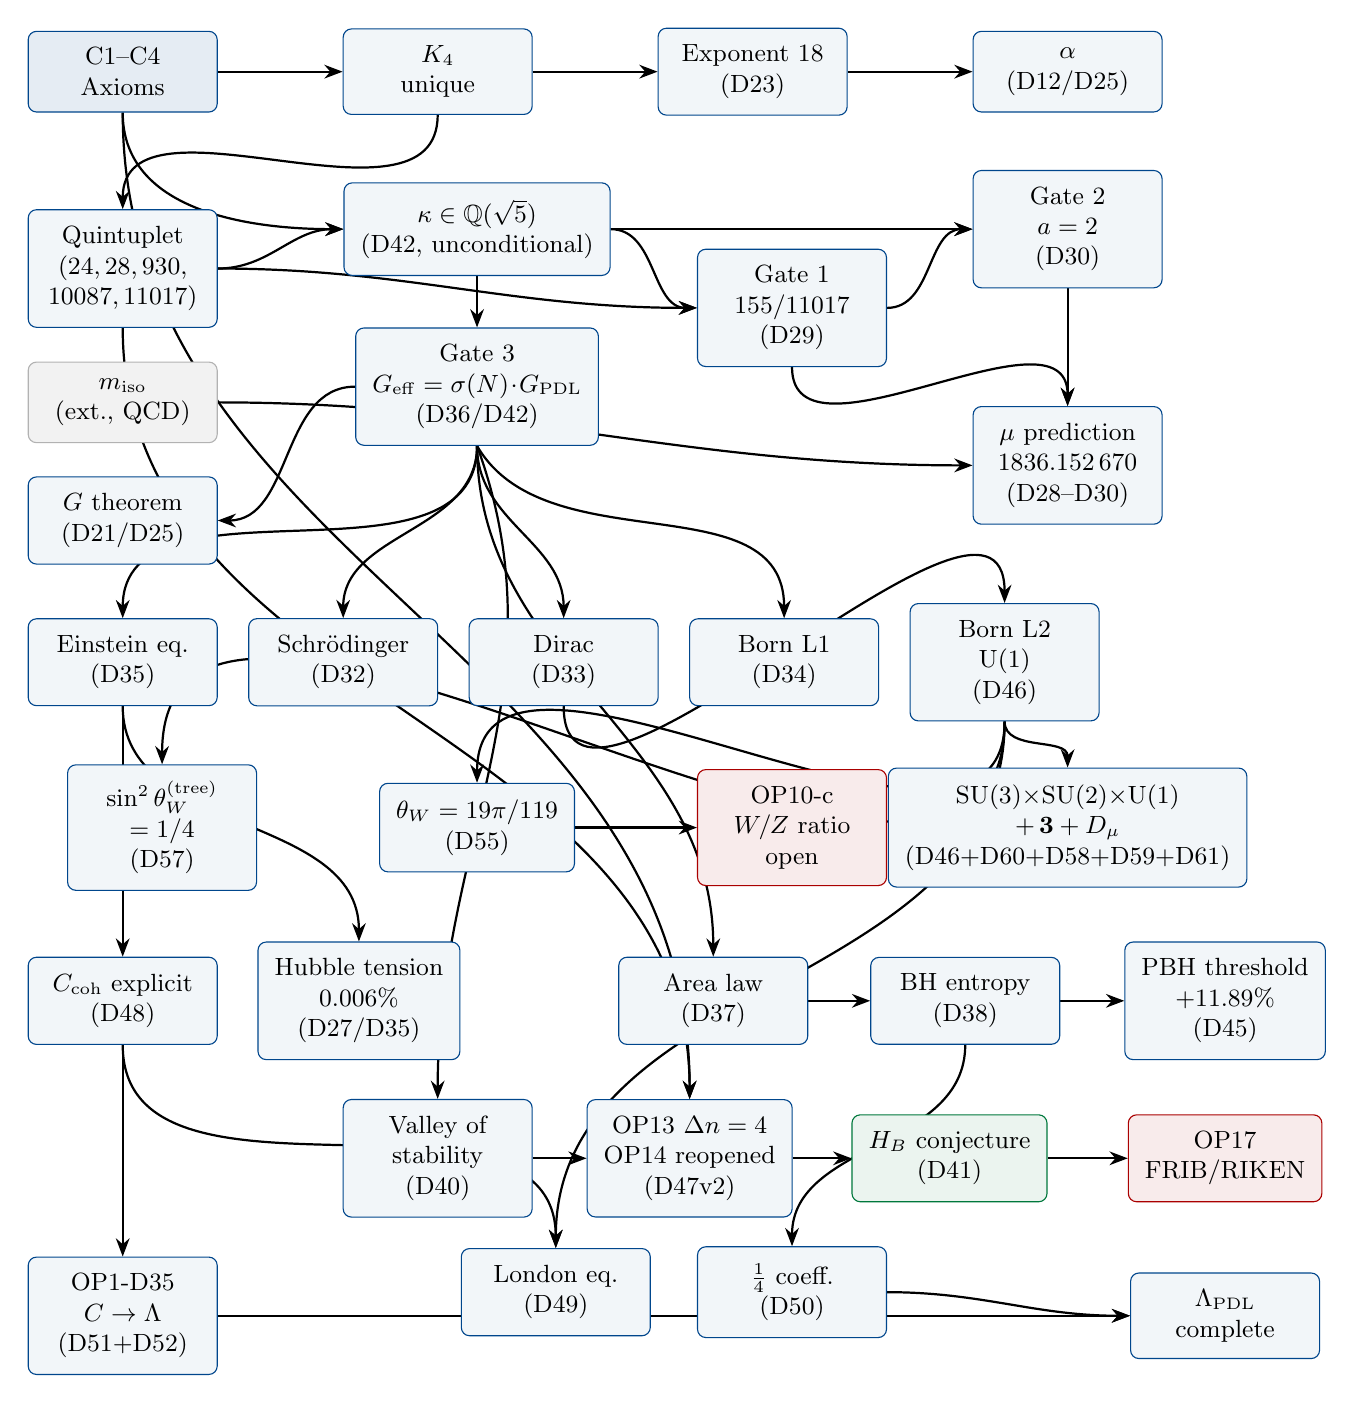
\begin{tikzpicture}[
  every node/.style={font=\small},
  axiom/.style={draw=proofblue, fill=proofblue!10,
    rounded corners=3pt, align=center, inner sep=6pt,
    minimum width=2.4cm, minimum height=0.9cm},
  theorem/.style={draw=proofblue, fill=proofblue!5,
    rounded corners=3pt, align=center, inner sep=6pt,
    minimum width=2.4cm, minimum height=0.9cm},
  conjecture/.style={draw=conjecturegreen, fill=conjecturegreen!8,
    rounded corners=3pt, align=center, inner sep=6pt,
    minimum width=2.4cm, minimum height=0.9cm},
  open/.style={draw=openproblemred, fill=openproblemred!8,
    rounded corners=3pt, align=center, inner sep=6pt,
    minimum width=2.4cm, minimum height=0.9cm},
  ext/.style={draw=gray!60, fill=gray!10,
    rounded corners=3pt, align=center, inner sep=6pt,
    minimum width=2.4cm, minimum height=0.9cm},
  arr/.style={-Stealth, thick},
]

% ── ROW 0 ── Axioms → K4 → Exp18 → alpha
\node[axiom]   at ( 0.0,  0.0) (C1C4)      {C1--C4\\Axioms};
\node[theorem] at ( 4.0,  0.0) (K4)        {$K_4$\\unique};
\node[theorem] at ( 8.0,  0.0) (exp18)     {Exponent~18\\(D23)};
\node[theorem] at (12.0,  0.0) (alpha)     {$\alpha$\\(D12/D25)};

% ── ROW 1 ── Quintuplet + kappa
\node[theorem] at ( 0.0, -2.5) (quintuplet){Quintuplet\\$(24,28,930,$\\$10087,11017)$};
\node[theorem] at ( 4.5, -2.0) (kappa)     {$\kappa\in\mathbb{Q}(\sqrt{5})$\\(D42, unconditional)};

% ── ROW 2 ── Gate1 + Gate2
\node[theorem] at ( 8.5, -3.0) (Gate1)     {Gate~1\\$155/11017$\\(D29)};
\node[theorem] at (12.0, -2.0) (Gate2)     {Gate~2\\$a=2$\\(D30)};

% ── ROW 3 ── miso + G + Gate3 + mu
\node[ext]     at ( 0.0, -4.2) (miso)      {$m_{\mathrm{iso}}$\\(ext., QCD)};
\node[theorem] at ( 0.0, -5.7) (G)         {$G$ theorem\\(D21/D25)};
\node[theorem] at ( 4.5, -4.0) (Gate3)     {Gate~3\\$G_{\mathrm{eff}}=\sigma(N)\!\cdot\!G_{\mathrm{PDL}}$\\(D36/D42)};
\node[theorem] at (12.0, -5.0) (mu)        {$\mu$ prediction\\$1836.152\,670$\\(D28--D30)};

% ── ROW 4 ── Einstein + Schrod + Dirac + Born L1 + Born L2
\node[theorem] at ( 0.0,-7.5) (Einstein)  {Einstein eq.\\(D35)};
\node[theorem] at ( 2.8,-7.5) (Schrod)    {Schr\"odinger\\(D32)};
\node[theorem] at ( 5.6,-7.5) (Dirac)     {Dirac\\(D33)};
\node[theorem] at ( 8.4,-7.5) (BornL1)    {Born L1\\(D34)};
\node[theorem] at (11.2,-7.5) (BornL2)    {Born L2\\U(1)\\(D46)};

% ── ROW 4b ── Electroweak: Weinberg + WZ open
\node[theorem] at ( 0.5,-9.6) (D57tree)  {$\sin^2\theta_W^{(\mathrm{tree})}$\\$=1/4$\\(D57)};
\node[theorem] at ( 4.5,-9.6) (D55node)  {$\theta_W=19\pi/119$\\(D55)};
\node[open]    at ( 8.5,-9.6) (WZopen)   {OP10-c\\$W/Z$ ratio\\open};
\node[theorem] at (12.0,-9.6) (SMgauge)  {$\SUthree{\times}\SUtwo{\times}\Uone$\\$+\,\mathbf{3}+D_\mu$\\(D46+D60+D58+D59+D61)};

% ── ROW 5 ── Ccoh + Hubble + AreaLaw + BH + D45
\node[theorem] at ( 0.0,-11.8) (Ccoh)     {$C_{\mathrm{coh}}$ explicit\\(D48)};
\node[theorem] at ( 3.0,-11.8) (Hubble)   {Hubble tension\\$0.006\%$\\(D27/D35)};
\node[theorem] at ( 7.5,-11.8) (AreaLaw)  {Area law\\(D37)};
\node[theorem] at (10.7,-11.8) (BH)       {BH entropy\\(D38)};
\node[theorem] at (14.0,-11.8) (D45)      {PBH threshold\\$+11.89\%$\\(D45)};

% ── ROW 6 ── Nuclear + D47 + HB + OP17
\node[theorem]    at ( 4.0,-13.8) (Nuclear) {Valley of\\stability\\(D40)};
\node[theorem]    at ( 7.2,-13.8) (D47node) {OP13 $\Delta n=4$\\OP14 reopened\\(D47v2)};
\node[conjecture] at (10.5,-13.8) (HB)      {$H_B$ conjecture\\(D41)};
\node[open]       at (14.0,-13.8) (OP17)    {OP17\\FRIB/RIKEN};

% ── ROW 7 ── D49 + D50 + D51/D52 + Lambda
\node[theorem] at ( 0.0,-15.8) (D51D52)  {OP1-D35\\$C\to\Lambda$\\(D51+D52)};
\node[theorem] at ( 5.5,-15.5) (D49)     {London eq.\\(D49)};
\node[theorem] at ( 8.5,-15.5) (D50)     {$\tfrac{1}{4}$ coeff.\\(D50)};
\node[theorem] at (14.0,-15.8) (Lambda)  {$\Lambda_{\mathrm{PDL}}$\\complete};

%% ══════════════════ FLÈCHES ══════════════════
\begin{pgfonlayer}{background}

% Row 0
\draw[arr] (C1C4.east)       -- (K4.west);
\draw[arr] (K4.east)         -- (exp18.west);
\draw[arr] (exp18.east)      -- (alpha.west);

% K4 → Quintuplet
\draw[arr] (K4.south)        to[out=-90, in=90] (quintuplet.north);

% Quintuplet + C1C4 → kappa
\draw[arr] (quintuplet.east) to[out=0, in=180] (kappa.west);
\draw[arr] (C1C4.south)      to[out=-90, in=180] (kappa.west);

% kappa + Quintuplet → Gate1
\draw[arr] (kappa.east)      to[out=0, in=180] (Gate1.west);
\draw[arr] (quintuplet.east) to[out=0, in=180] (Gate1.west);

% Gate1 → Gate2, kappa → Gate2
\draw[arr] (Gate1.east)      to[out=0, in=180] (Gate2.west);
\draw[arr] (kappa.east)      to[out=0, in=180] (Gate2.west);

% kappa → Gate3
\draw[arr] (kappa.south)     -- (Gate3.north);

% Gate3 → G
\draw[arr] (Gate3.west)      to[out=180, in=0] (G.east);

% Gate1 + Gate2 + miso → mu
\draw[arr] (Gate1.south)     to[out=-90, in=90]  (mu.north);
\draw[arr] (Gate2.south)     to[out=-90, in=90]  (mu.north);
\draw[arr] (miso.east)       to[out=0,   in=180] (mu.west);

% Gate3 → dynamics (row 4)
\draw[arr] (Gate3.south)     to[out=-90, in=90] (Einstein.north);
\draw[arr] (Gate3.south)     to[out=-90, in=90] (Schrod.north);
\draw[arr] (Gate3.south)     to[out=-90, in=90] (Dirac.north);
\draw[arr] (Gate3.south)     to[out=-60, in=90] (BornL1.north);
\draw[arr] (Dirac.south)     to[out=-90, in=90] (BornL2.north);

% Electroweak
\draw[arr] (BornL2.south)    to[out=-90, in=90] (D57tree.north);
\draw[arr] (BornL2.south)    to[out=-90, in=90] (D55node.north);
\draw[arr] (D55node.east)    -- (WZopen.west);
\draw[arr] (BornL2.south)    to[out=-90, in=90] (SMgauge.north);

% Einstein → Ccoh, Hubble
\draw[arr] (Einstein.south)  -- (Ccoh.north);
\draw[arr] (Einstein.south)  to[out=-90, in=90] (Hubble.north);

% Ccoh → D49, D51D52
\draw[arr] (Ccoh.south)      -- (D51D52.north);
\draw[arr] (Ccoh.south)      to[out=-90, in=90] (D49.north);
\draw[arr] (BornL2.south)    to[out=-90, in=90] (D49.north);

% Gate3 → AreaLaw
\draw[arr] (Gate3.south)     to[out=-90, in=90] (AreaLaw.north);

% AreaLaw → BH
\draw[arr] (AreaLaw.east)    -- (BH.west);

% BH → D45, D50
\draw[arr] (BH.east)         -- (D45.west);
\draw[arr] (BH.south)        to[out=-90, in=90] (D50.north);

% Gate3 → Nuclear
\draw[arr] (Gate3.south)     to[out=-70, in=90] (Nuclear.north);

% Quintuplet + C1C4 → D47
\draw[arr] (quintuplet.south) to[out=-90, in=90] (D47node.north);
\draw[arr] (C1C4.south)       to[out=-90, in=90] (D47node.north);

% Nuclear + D47 → HB
\draw[arr] (Nuclear.east)    -- (D47node.west);
\draw[arr] (D47node.east)    -- (HB.west);

% D51D52 + D50 → Lambda
\draw[arr] (D51D52.east)     to[out=0, in=180] (Lambda.west);
\draw[arr] (D50.east)        to[out=0, in=180] (Lambda.west);

% HB → OP17
\draw[arr] (HB.east)         -- (OP17.west);

\end{pgfonlayer}
\end{tikzpicture}%
}
\caption{Critical-path dependency map of the PDL programme --- foundational chain (v31). \textcolor{proofblue}{Blue}: unconditional theorems. \textcolor{conjecturegreen}{Green}: conjectures. \textcolor{openproblemred}{Red}: open problems. Grey: unique external input ($m_{\mathrm{iso}}$). The quantum dynamics layer (Schr\"odinger, Dirac, Born, London), nuclear stability, black hole thermodynamics, and cosmological constant are complete theorems of C1--C4. The gauge sector node (bottom right) is a summary; the full derivation chain $K_4 \to D_\mu$ is detailed in Figure~\ref{fig:dependency_gauge}.}
\label{fig:dependency_main}
\end{figure}

\clearpage

% ──────────────────────────────────────────────────────────────
% FIGURE 2 — Gauge sector: K4 → G_gauge → D_mu
% ──────────────────────────────────────────────────────────────
\begin{figure}[H]
\centering
\resizebox{0.97\textwidth}{!}{%
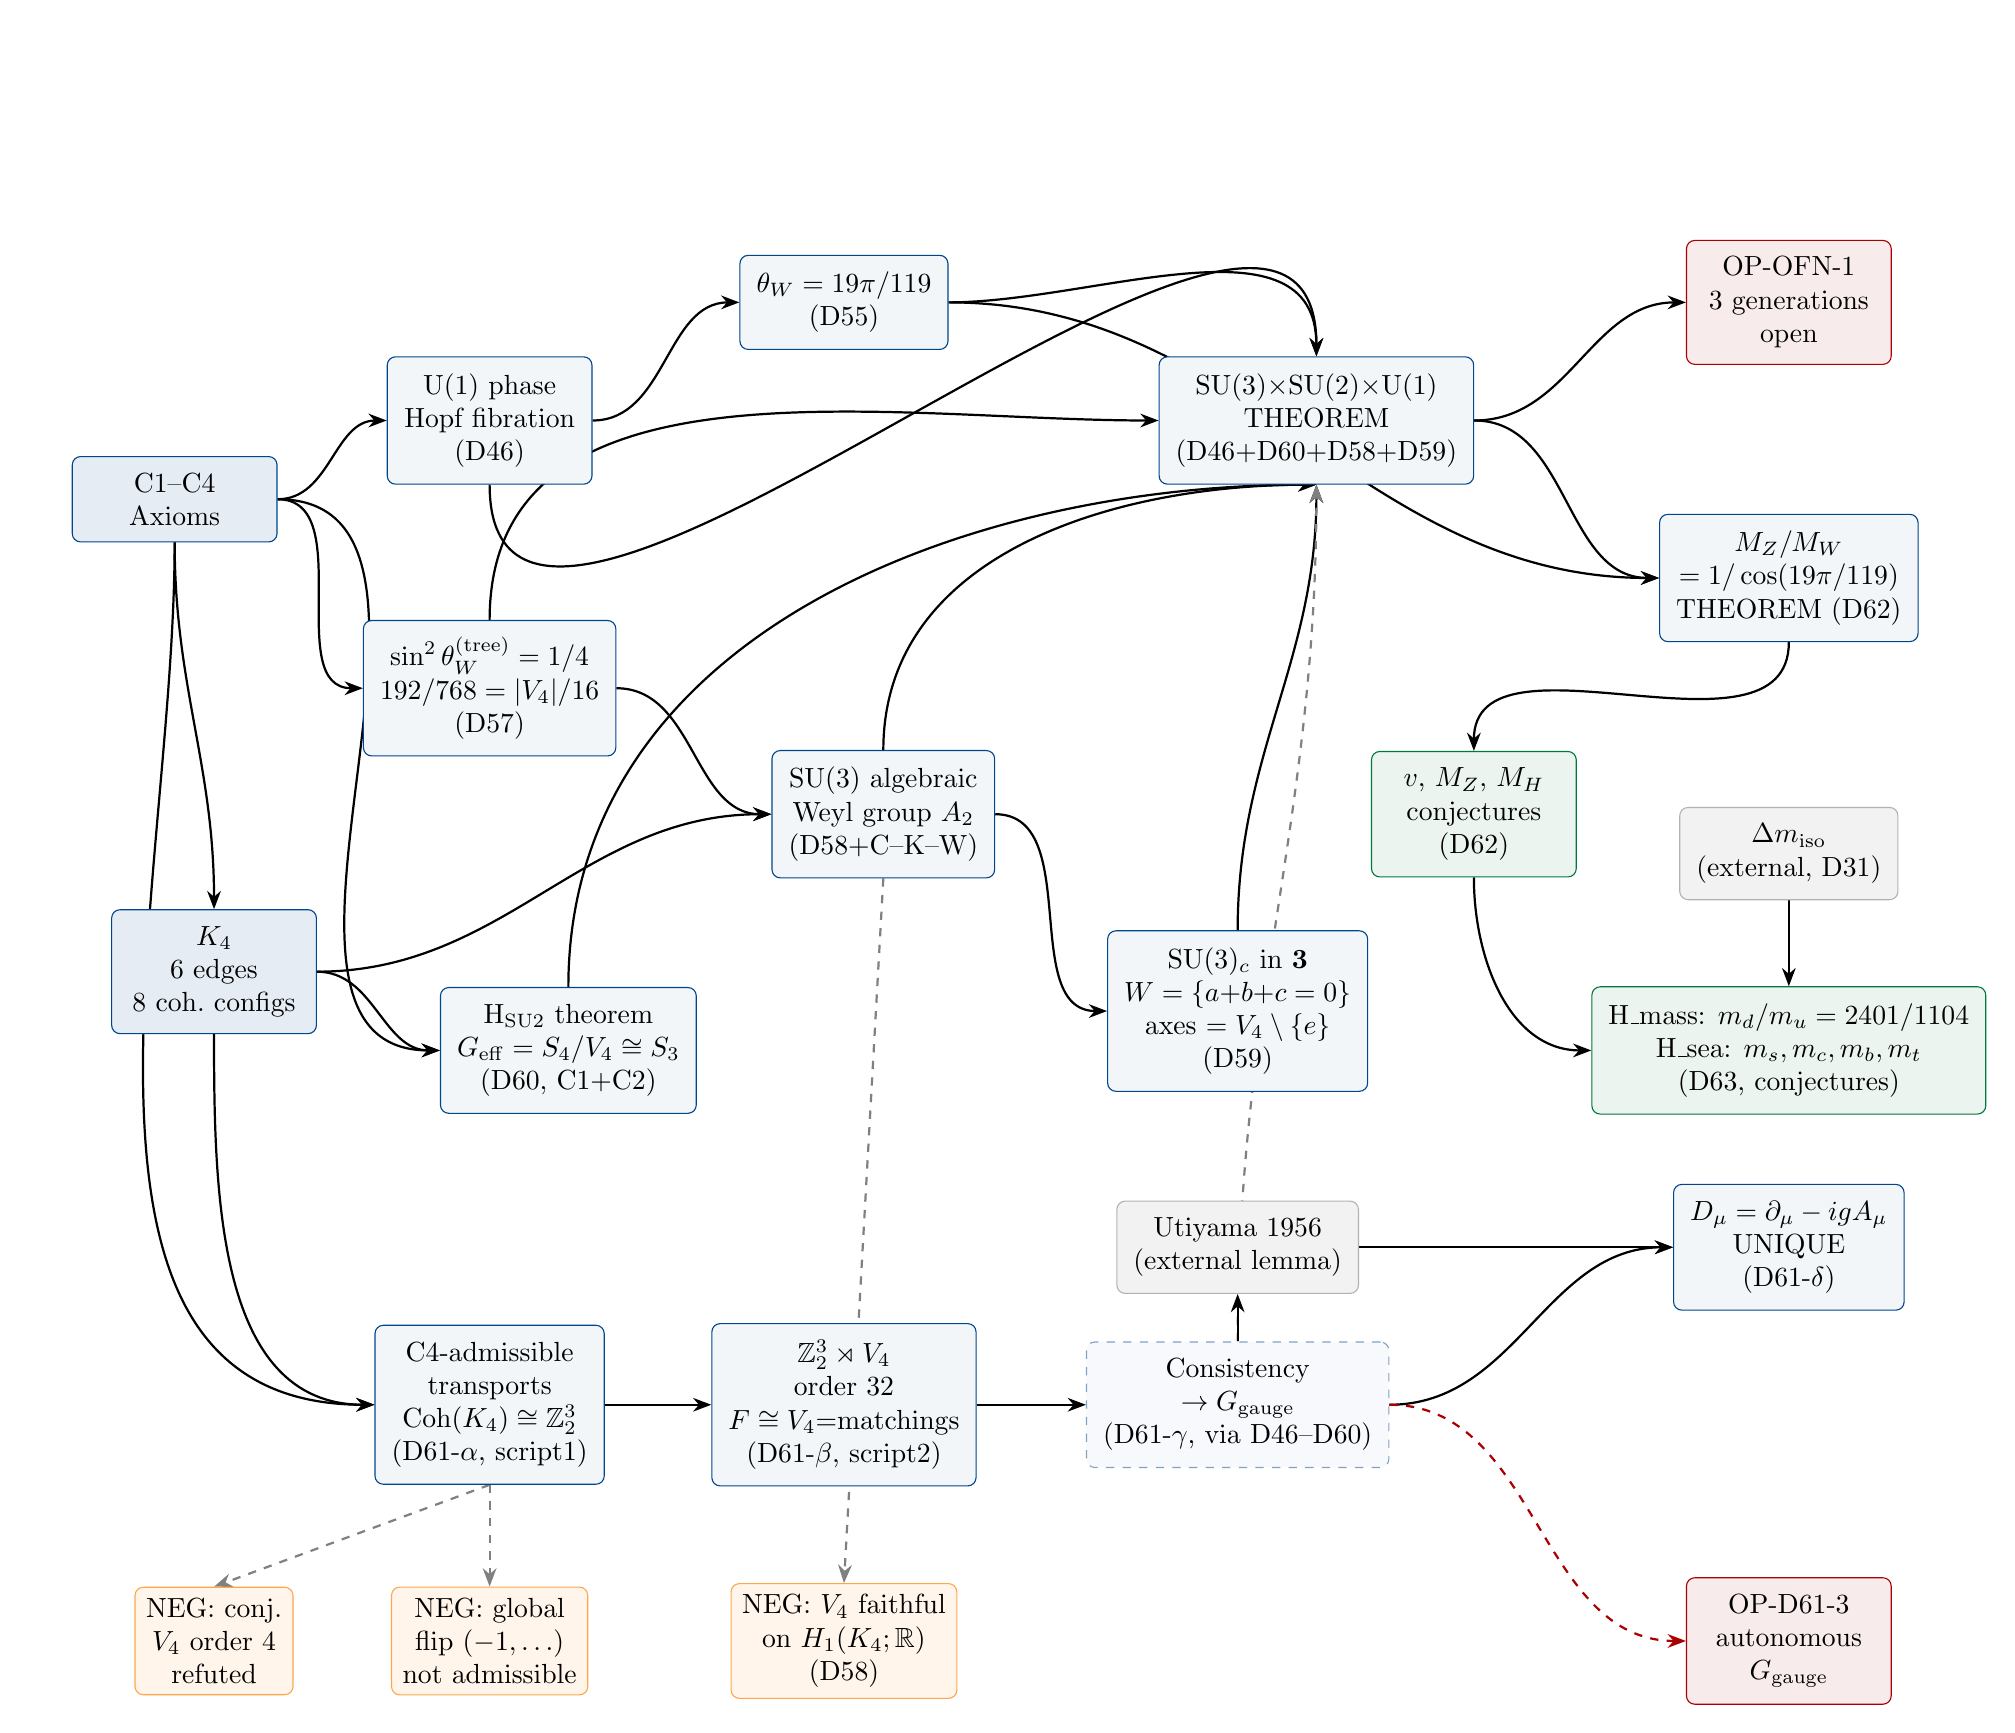
\begin{tikzpicture}[
  every node/.style={font=\normalsize},
  axiom/.style={draw=proofblue, fill=proofblue!10,
    rounded corners=3pt, align=center, inner sep=6pt,
    minimum width=2.6cm, minimum height=0.9cm},
  theorem/.style={draw=proofblue, fill=proofblue!5,
    rounded corners=3pt, align=center, inner sep=6pt,
    minimum width=2.6cm, minimum height=0.9cm},
  consist/.style={draw=proofblue!50, fill=proofblue!3,
    rounded corners=3pt, align=center, inner sep=6pt,
    minimum width=2.6cm, minimum height=0.9cm,
    dashed},
  conjecture/.style={draw=conjecturegreen, fill=conjecturegreen!8,
    rounded corners=3pt, align=center, inner sep=6pt,
    minimum width=2.6cm, minimum height=0.9cm},
  ext/.style={draw=gray!60, fill=gray!10,
    rounded corners=3pt, align=center, inner sep=6pt,
    minimum width=2.6cm, minimum height=0.9cm},
  open/.style={draw=openproblemred, fill=openproblemred!8,
    rounded corners=3pt, align=center, inner sep=6pt,
    minimum width=2.6cm, minimum height=0.9cm},
  neg/.style={draw=orange!70, fill=orange!8,
    rounded corners=3pt, align=center, inner sep=4pt,
    minimum width=2.0cm, minimum height=0.7cm},
  arr/.style={-Stealth, thick},
  arrext/.style={-Stealth, thick, dashed, gray},
]

% ── COL 0 : Axiomes
\node[axiom]   at ( 0.0,  0.0) (C1C4)   {C1--C4\\Axioms};
\node[axiom]   at ( 0.5, -6.0) (K4)     {$K_4$\\6 edges\\8 coh.\ configs};

% ── COL 1 : U(1) branch (D46)
\node[theorem] at ( 4.0,  1.0) (U1)     {$\Uone$ phase\\Hopf fibration\\(D46)};

% ── COL 1b : D57 Weinberg tree
\node[theorem] at ( 4.0, -2.4) (D57)    {$\sin^2\theta_W^{(\mathrm{tree})}=1/4$\\$192/768 = |V_4|/16$\\(D57)};

% ── COL 1c : D60 H_SU2
\node[theorem] at ( 5.0, -7.0) (D60)    {H$_{\mathrm{SU2}}$ theorem\\$G_{\mathrm{eff}}=S_4/V_4\cong S_3$\\(D60, C1+C2)};

% ── COL 2 : D58 SU(3)
\node[theorem] at ( 9.0, -4.0) (D58)    {$\SUthree$ algebraic\\Weyl group $A_2$\\(D58+C--K--W)};

% ── COL 2b : D55 Weinberg
\node[theorem] at ( 8.5,  2.5) (D55)    {$\theta_W=19\pi/119$\\(D55)};

% ── COL 3 : D59 representation 3
\node[theorem] at (13.5, -6.5) (D59)    {$\SUthree_c$ in $\mathbf{3}$\\$W=\{a{+}b{+}c=0\}$\\axes $=V_4\setminus\{e\}$\\(D59)};

% ── COL 3b : G_gauge as theorem
\node[theorem] at (14.5,  1.0) (Ggauge) {$\SUthree{\times}\SUtwo{\times}\Uone$\\THEOREM\\(D46+D60+D58+D59)};

% ── GAUGE TRANSPORT CHAIN (D61) — Row below
\node[theorem] at ( 4.0, -11.5) (alpha)  {C4-admissible\\transports\\$\Coh\cong\mathbb{Z}_2^3$\\(D61-$\alpha$, script1)};
\node[theorem] at ( 8.5, -11.5) (beta)   {$\mathbb{Z}_2^3\rtimes V_4$\\order 32\\$F\cong V_4$=matchings\\(D61-$\beta$, script2)};
\node[consist] at (13.5, -11.5) (gamma)  {Consistency\\$\to G_{\mathrm{gauge}}$\\(D61-$\gamma$, via D46--D60)};
\node[ext]     at (13.5, -9.5) (Utiyama){Utiyama 1956\\(external lemma)};
\node[theorem] at (20.5, -9.5) (Dmu)    {$\Dmu=\partial_\mu-igA_\mu$\\UNIQUE\\(D61-$\delta$)};

% ── COL 4 : D62 gauge boson masses [NEW v29]
\node[theorem]    at (20.5, -1.0) (D62mass) {$M_Z/M_W$\\$=1/\cos(19\pi/119)$\\THEOREM (D62)};
\node[conjecture] at (16.5, -4.0) (D62conj) {$v$, $M_Z$, $M_H$\\conjectures\\(D62)};

% ── COL 4b : D63 quark masses [NEW v29]
\node[conjecture] at (20.5, -7.0) (D63node) {H\_mass: $m_d/m_u=2401/1104$\\H\_sea: $m_s,m_c,m_b,m_t$\\(D63, conjectures)};
\node[ext]        at (20.5, -4.5) (miso_ext){$\Delta m_{\mathrm{iso}}$\\(external, D31)};

% ── Negative results
\node[neg] at ( 0.5, -14.5) (neg1) {NEG: conj.\\$V_4$ order 4\\refuted};
\node[neg] at ( 4.0, -14.5) (neg2) {NEG: global\\flip $(-1,\ldots)$\\not admissible};
\node[neg] at ( 8.5, -14.5) (neg3) {NEG: $V_4$ faithful\\on $H_1(K_4;\mathbb{R})$\\(D58)};

% ── Remaining open problems
\node[open] at (20.5,  2.5) (OPOFN)  {OP-OFN-1\\3 generations\\open};
\node[open] at (20.5, -14.5) (OP61c)  {OP-D61-3\\autonomous\\$G_{\mathrm{gauge}}$};

%% ══════════════════ FLÈCHES ══════════════════
\begin{pgfonlayer}{background}

% C1C4 → K4, U1, D57, D60
\draw[arr] (C1C4.south)   to[out=-90,in=90] (K4.north);
\draw[arr] (C1C4.east)    to[out=0,in=180] (U1.west);
\draw[arr] (C1C4.east)    to[out=0,in=180] (D57.west);
\draw[arr] (C1C4.east)    to[out=0,in=180] (D60.west);

% K4 → D58, D60, alpha
\draw[arr] (K4.east)      to[out=0,in=180] (D58.west);
\draw[arr] (K4.east)      to[out=0,in=180] (D60.west);
\draw[arr] (K4.south)     to[out=-90,in=180] (alpha.west);

% U1 → D55, Ggauge
\draw[arr] (U1.east)      to[out=0,in=180] (D55.west);
\draw[arr] (U1.south)     to[out=-90,in=90] (Ggauge.north);

% D57 → D58, Ggauge
\draw[arr] (D57.east)     to[out=0,in=180] (D58.west);
\draw[arr] (D57.north)    to[out=90,in=180] (Ggauge.west);

% D60 → Ggauge
\draw[arr] (D60.north)    to[out=90,in=180] (Ggauge.south);

% D58 → D59, Ggauge
\draw[arr] (D58.east)     to[out=0,in=180] (D59.west);
\draw[arr] (D58.north)    to[out=90,in=180] (Ggauge.south);

% D59 → Ggauge
\draw[arr] (D59.north)    to[out=90,in=-90] (Ggauge.south);

% D55 → Ggauge
\draw[arr] (D55.east)     to[out=0,in=90] (Ggauge.north);

% Ggauge → D62mass (theorem, OP10-c resolved), OPOFN
\draw[arr] (Ggauge.east)  to[out=0,in=180] (D62mass.west);
\draw[arr] (Ggauge.east)  to[out=0,in=180] (OPOFN.west);

% D55 → D62mass (Weinberg angle used in ratio)
\draw[arr] (D55.east)     to[out=0,in=180] (D62mass.west);

% D62mass → D62conj (theorem feeds conjectures)
\draw[arr] (D62mass.south) to[out=-90,in=90] (D62conj.north);

% D63: D62conj + miso_ext → D63node
\draw[arr] (D62conj.south)  to[out=-90,in=180] (D63node.west);
\draw[arr] (miso_ext.south) -- (D63node.north);

% D61 chain: alpha → beta → gamma → delta → Dmu
\draw[arr] (alpha.east)   -- (beta.west);
\draw[arr] (beta.east)    -- (gamma.west);
\draw[arrext] (gamma.north) to[out=90,in=-90] (Ggauge.south);
\draw[arr] (gamma.north)  to[out=90,in=-90] (Utiyama.south);
\draw[arr] (gamma.east)   to[out=0,in=180] (Dmu.west);
\draw[arr] (Utiyama.east) -- (Dmu.west);

% C4 → alpha (survival principle)
\draw[arr] (C1C4.south)   to[out=-90,in=180] (alpha.west);

% Negative results
\draw[arr,dashed,gray] (alpha.south) -- (neg1.north);
\draw[arr,dashed,gray] (alpha.south) -- (neg2.north);
\draw[arr,dashed,gray] (D58.south)   -- (neg3.north);

% OP-D61-3
\draw[arr,dashed,openproblemred] (gamma.east) to[out=0,in=180] (OP61c.west);

\end{pgfonlayer}
\end{tikzpicture}%
}
\caption{Gauge sector dependency map of the PDL programme (v29). \textcolor{proofblue}{Blue solid}: unconditional theorems. \textcolor{conjecturegreen}{Green}: motivated conjectures. \textbf{Blue dashed}: consistency result (arrow~$\gamma$ of D61). Grey: external lemma (Utiyama 1956) and external parameter ($\Delta m_{\mathrm{iso}}$). \textcolor{openproblemred}{Red}: open problems. Orange: documented negative results. The four arrows of the D61 causal chain are labelled $\alpha$--$\delta$. \textbf{New in v29}: OP10-c ($W/Z$ mass ratio) is resolved by D62 as the unconditional theorem $M_Z/M_W = 1/\cos(19\pi/119)$; the electroweak vev $v$, $M_Z$, and $M_H$ are derived as motivated conjectures (D62); the quark mass spectrum is addressed by Conjectures H\_mass and H\_sea (D63), with sole external input $\Delta m_{\mathrm{iso}}$ (D31). OP-OFN-1 (three fermion generations) remains open.}
\label{fig:dependency_gauge}
\end{figure}

\clearpage

% ──────────────────────────────────────────────────────────────
% FIGURE 3 — Black hole physics II: D64-D65 dependency chain
% ──────────────────────────────────────────────────────────────
\begin{figure}[H]
\centering
\resizebox{0.85\textwidth}{!}{%
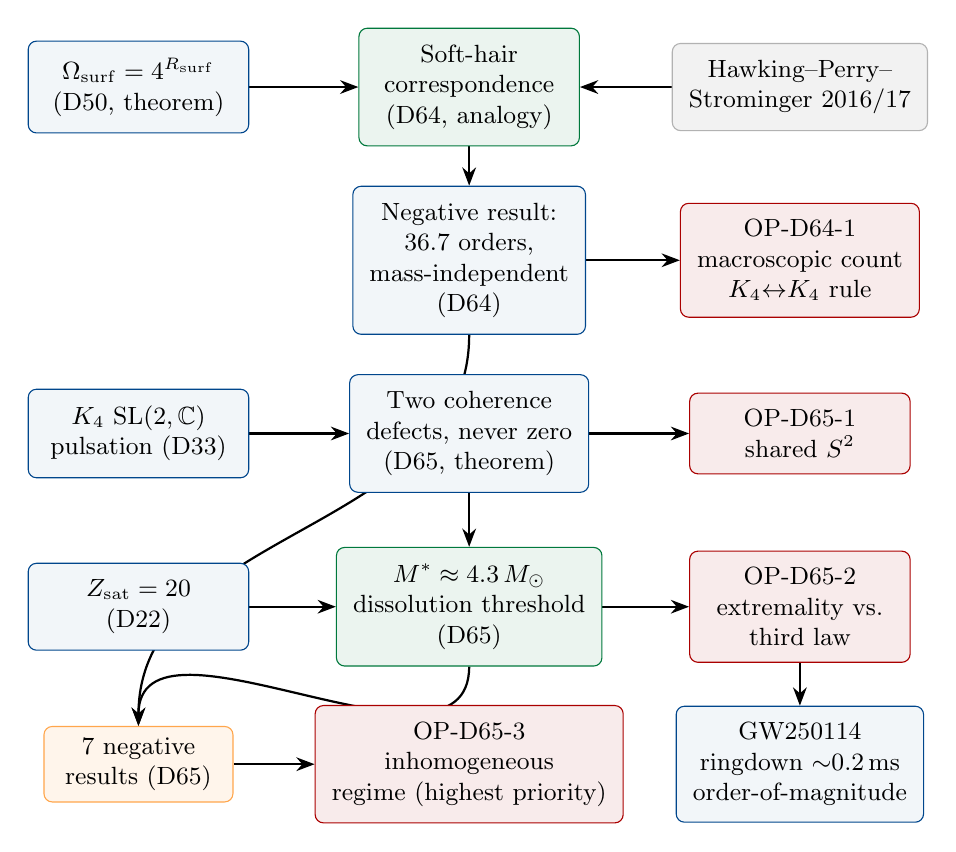
\begin{tikzpicture}[
  every node/.style={font=\small},
  theorem/.style={draw=proofblue, fill=proofblue!5,
    rounded corners=3pt, align=center, inner sep=6pt,
    minimum width=2.8cm, minimum height=0.9cm},
  conjecture/.style={draw=conjecturegreen, fill=conjecturegreen!8,
    rounded corners=3pt, align=center, inner sep=6pt,
    minimum width=2.8cm, minimum height=0.9cm},
  open/.style={draw=openproblemred, fill=openproblemred!8,
    rounded corners=3pt, align=center, inner sep=6pt,
    minimum width=2.8cm, minimum height=0.9cm},
  neg/.style={draw=orange!70, fill=orange!8,
    rounded corners=3pt, align=center, inner sep=4pt,
    minimum width=2.4cm, minimum height=0.7cm},
  ext/.style={draw=gray!60, fill=gray!10,
    rounded corners=3pt, align=center, inner sep=6pt,
    minimum width=2.8cm, minimum height=0.9cm},
  arr/.style={-Stealth, thick},
]

\node[theorem]  at ( 0.0,  0.0) (D50)    {$\Omega_{\mathrm{surf}}=4^{\Rsurf}$\\(D50, theorem)};
\node[conjecture] at ( 4.2, 0.0) (soft)  {Soft-hair\\correspondence\\(D64, analogy)};
\node[ext]      at ( 8.4,  0.0) (HPS)    {Hawking--Perry--\\Strominger 2016/17};
\node[theorem]  at ( 4.2, -2.2) (neg1)   {Negative result:\\$36.7$ orders,\\mass-independent\\(D64)};
\node[open]     at ( 8.4, -2.2) (OP641)  {OP-D64-1\\macroscopic count\\$K_4{\leftrightarrow}K_4$ rule};

\node[theorem]  at ( 0.0, -4.4) (K4pulse) {$\Kfour$ $\mathrm{SL}(2,\mathbb{C})$\\pulsation (D33)};
\node[theorem]  at ( 4.2, -4.4) (defects) {Two coherence\\defects, never zero\\(D65, theorem)};
\node[open]     at ( 8.4, -4.4) (OPS2)    {OP-D65-1\\shared $S^2$};

\node[theorem]  at ( 0.0, -6.6) (Zsat)    {$\Zsat=20$\\(D22)};
\node[conjecture] at ( 4.2, -6.6) (Mstar) {$M^*\approx4.3\,M_\odot$\\dissolution threshold\\(D65)};
\node[open]     at ( 8.4, -6.6) (OPext)   {OP-D65-2\\extremality vs.\\third law};

\node[neg]      at ( 0.0, -8.6) (sevenneg) {7 negative\\results (D65)};
\node[open]     at ( 4.2, -8.6) (OP653)    {OP-D65-3\\inhomogeneous\\regime (highest priority)};
\node[theorem]  at ( 8.4, -8.6) (GW250114) {GW250114\\ringdown $\sim$0.2\,ms\\order-of-magnitude};

\begin{pgfonlayer}{background}
\draw[arr] (D50.east)     -- (soft.west);
\draw[arr] (HPS.west)     -- (soft.east);
\draw[arr] (soft.south)   -- (neg1.north);
\draw[arr] (neg1.east)    -- (OP641.west);
\draw[arr] (K4pulse.east) -- (defects.west);
\draw[arr] (defects.east) -- (OPS2.west);
\draw[arr] (Zsat.east)    -- (Mstar.west);
\draw[arr] (defects.south) to[out=-90,in=90] (Mstar.north);
\draw[arr] (Mstar.east)   -- (OPext.west);
\draw[arr] (neg1.south)   to[out=-90,in=90] (sevenneg.north);
\draw[arr] (Mstar.south)  to[out=-90,in=90] (sevenneg.north);
\draw[arr] (sevenneg.east) -- (OP653.west);
\draw[arr] (OPext.south)  to[out=-90,in=90] (GW250114.north);
\end{pgfonlayer}
\end{tikzpicture}%
}
\caption{Black hole physics II dependency chain (new in v30). \textcolor{proofblue}{Blue}: unconditional theorems. \textcolor{conjecturegreen}{Green}: conjectures. Orange: documented negative results. \textcolor{openproblemred}{Red}: open problems. Grey: external literature (soft hair). The programme moves from the D50 surface-degeneracy theorem, through the D64 soft-hair analogy and its honest negative result, to the D65 behavioural theorems (two coherence defects, curvature-migration exponent, dissolution threshold) and their associated open problems. OP-D64-1 and OP-D65-3 are jointly the highest-priority entry points.}
\label{fig:dependency_bh2}
\end{figure}

\newpage

% ──────────────────────────────────────────────────────────────
% FIGURE 4 — D66: logical geometry on K4 and the search for a nucleon metric
% ──────────────────────────────────────────────────────────────
\begin{figure}[H]
\centering
\resizebox{0.9\textwidth}{!}{%
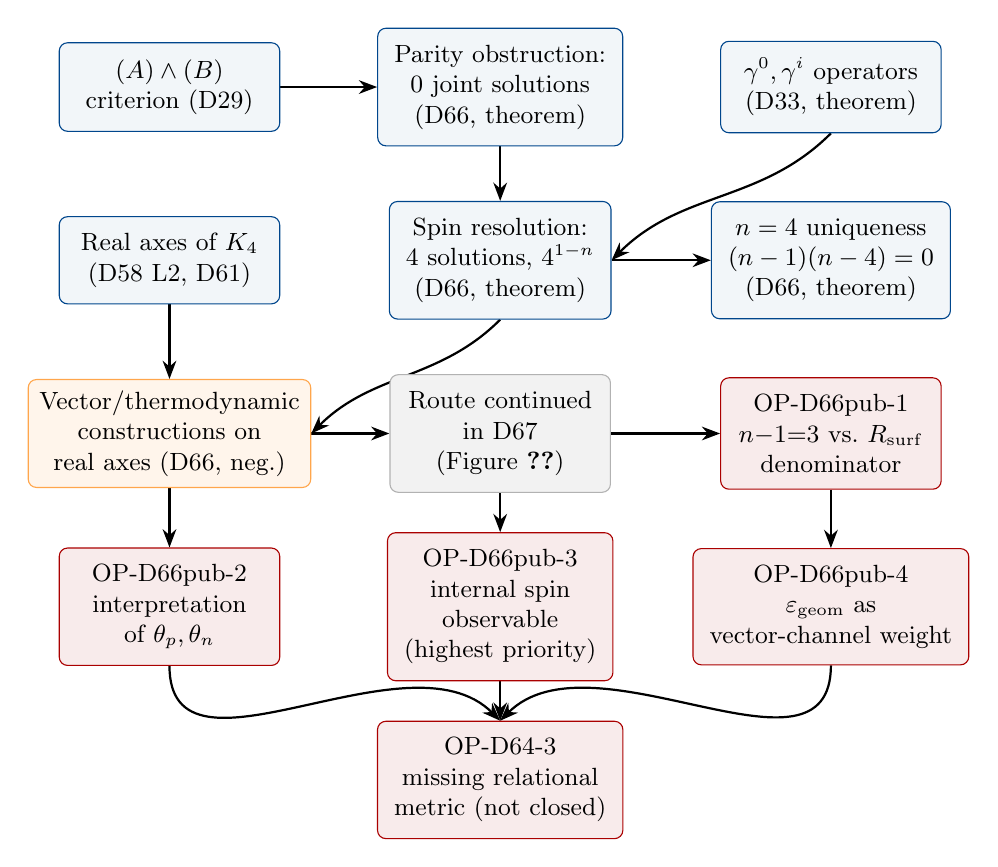
\begin{tikzpicture}[
  every node/.style={font=\small},
  theorem/.style={draw=proofblue, fill=proofblue!5,
    rounded corners=3pt, align=center, inner sep=6pt,
    minimum width=2.8cm, minimum height=0.9cm},
  conjecture/.style={draw=conjecturegreen, fill=conjecturegreen!8,
    rounded corners=3pt, align=center, inner sep=6pt,
    minimum width=2.8cm, minimum height=0.9cm},
  open/.style={draw=openproblemred, fill=openproblemred!8,
    rounded corners=3pt, align=center, inner sep=6pt,
    minimum width=2.8cm, minimum height=0.9cm},
  neg/.style={draw=orange!70, fill=orange!8,
    rounded corners=3pt, align=center, inner sep=4pt,
    minimum width=2.4cm, minimum height=0.7cm},
  ext/.style={draw=gray!60, fill=gray!10,
    rounded corners=3pt, align=center, inner sep=6pt,
    minimum width=2.8cm, minimum height=0.9cm},
  arr/.style={-Stealth, thick},
]

\node[theorem]  at ( 0.0,  0.0) (AB)      {$(A)\wedge(B)$\\criterion (D29)};
\node[theorem]  at ( 4.2,  0.0) (parity)  {Parity obstruction:\\0 joint solutions\\(D66, theorem)};
\node[theorem]  at ( 8.4,  0.0) (D33ops)  {$\gamma^0,\gamma^i$ operators\\(D33, theorem)};

\node[theorem]  at ( 0.0, -2.2) (axes)    {Real axes of $K_4$\\(D58 L2, D61)};
\node[theorem]  at ( 4.2, -2.2) (spinres) {Spin resolution:\\4 solutions, $4^{1-n}$\\(D66, theorem)};
\node[theorem]  at ( 8.4, -2.2) (n4uniq)  {$n=4$ uniqueness\\$(n-1)(n-4)=0$\\(D66, theorem)};

\node[neg]      at ( 0.0, -4.4) (vecconstr) {Vector/thermodynamic\\constructions on\\real axes (D66, neg.)};
\node[ext]      at ( 4.2, -4.4) (toD67)    {Route continued\\in D67\\(Figure~\ref{fig:dependency_D67})};
\node[open]     at ( 8.4, -4.4) (OPpub1)  {OP-D66pub-1\\$n{-}1{=}3$ vs.\ $\Rsurf$\\denominator};

\node[open]     at ( 0.0, -6.6) (OPpub2)  {OP-D66pub-2\\interpretation\\of $\theta_p,\theta_n$};
\node[open]     at ( 4.2, -6.6) (OPpub3)  {OP-D66pub-3\\internal spin\\observable\\(highest priority)};
\node[open]     at ( 8.4, -6.6) (OPpub4)  {OP-D66pub-4\\$\varepsilon_{\mathrm{geom}}$ as\\vector-channel weight};

\node[open]     at ( 4.2, -8.8) (OP643)   {OP-D64-3\\missing relational\\metric (not closed)};

\begin{pgfonlayer}{background}
\draw[arr] (AB.east)      -- (parity.west);
\draw[arr] (parity.south) -- (spinres.north);
\draw[arr] (D33ops.south) to[out=-135,in=45] (spinres.east);
\draw[arr] (spinres.east) -- (n4uniq.west);
\draw[arr] (axes.south)   -- (vecconstr.north);
\draw[arr] (spinres.south) to[out=-135,in=45] (vecconstr.east);
\draw[arr] (vecconstr.east) -- (toD67.west);
\draw[arr] (toD67.east)  -- (OPpub1.west);
\draw[arr] (vecconstr.south) -- (OPpub2.north);
\draw[arr] (toD67.south) -- (OPpub3.north);
\draw[arr] (OPpub1.south) -- (OPpub4.north);
\draw[arr] (OPpub2.south) to[out=-90,in=135] (OP643.north);
\draw[arr] (OPpub3.south) -- (OP643.north);
\draw[arr] (OPpub4.south) to[out=-90,in=45] (OP643.north);
\end{pgfonlayer}
\end{tikzpicture}%
}
\caption{Logical geometry on $K_4$ and the search for a nucleon metric: D66 dependency chain (new in v31). \textcolor{proofblue}{Blue}: unconditional theorems. Orange: documented negative results. \textcolor{openproblemred}{Red}: open problems. Grey: cross-reference to Figure~\ref{fig:dependency_D67}. The programme moves from the classical $(A)\wedge(B)$ criterion (D29) and the real axes of $K_4$ (D58, D61), through the parity-obstruction and spin-resolution theorems of D66 (linking to the pre-existing Dirac operators of D33) and the $n=4$ uniqueness theorem, to the documented family of negative vector constructions, whose curvature question is resolved --- negatively --- in D67 (Figure~\ref{fig:dependency_D67}). OP-D66pub-3 (an internally derived, orientation-dependent nucleon observable) is the highest-priority entry point among the four D66 open problems, all of which converge on the still-open OP-D64-3.}
\label{fig:dependency_D66}
\end{figure}

\newpage

% ──────────────────────────────────────────────────────────────
% FIGURE 5 — D67: coplanarity theorem, corrected closure relation,
% the 18=2x9 lead, and the isolated-nucleon open problems
% ──────────────────────────────────────────────────────────────
\begin{figure}[H]
\centering
\resizebox{0.92\textwidth}{!}{%
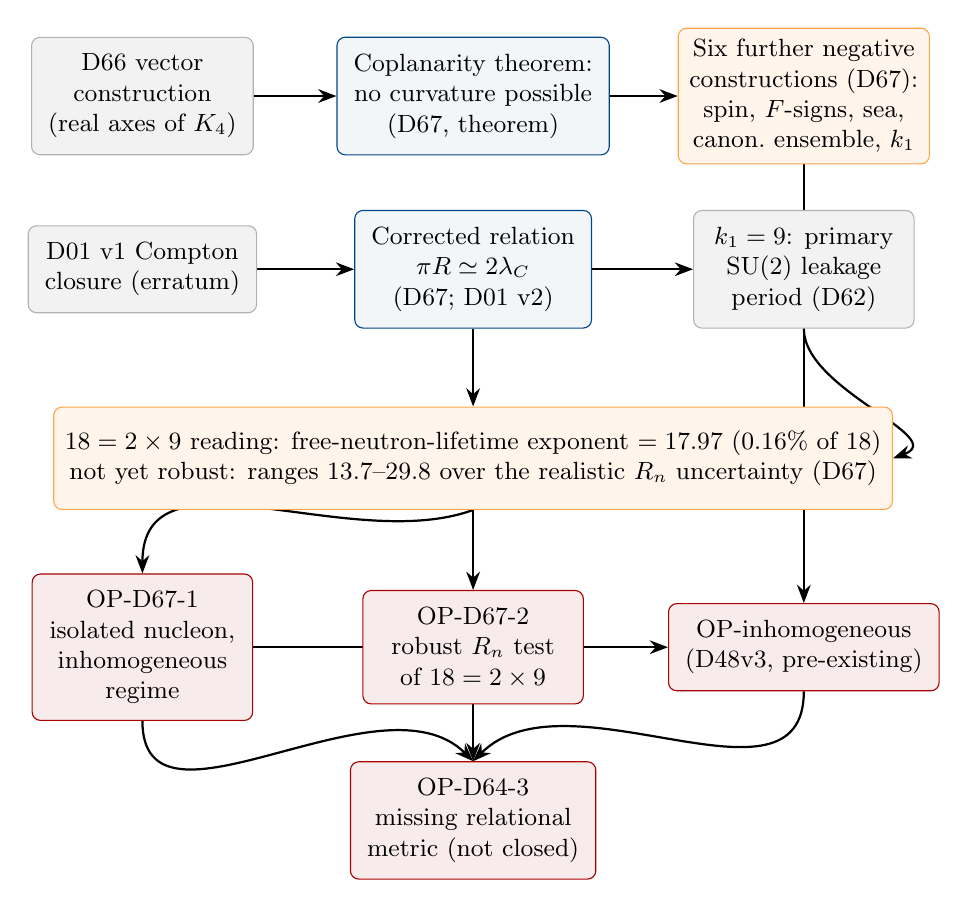
\begin{tikzpicture}[
  every node/.style={font=\small},
  theorem/.style={draw=proofblue, fill=proofblue!5,
    rounded corners=3pt, align=center, inner sep=6pt,
    minimum width=2.8cm, minimum height=0.9cm},
  open/.style={draw=openproblemred, fill=openproblemred!8,
    rounded corners=3pt, align=center, inner sep=6pt,
    minimum width=2.8cm, minimum height=0.9cm},
  neg/.style={draw=orange!70, fill=orange!8,
    rounded corners=3pt, align=center, inner sep=4pt,
    minimum width=2.6cm, minimum height=0.7cm},
  ext/.style={draw=gray!60, fill=gray!10,
    rounded corners=3pt, align=center, inner sep=6pt,
    minimum width=2.8cm, minimum height=0.9cm},
  arr/.style={-Stealth, thick},
]

\node[ext]      at ( 0.0,  0.0) (D66vec)  {D66 vector\\construction\\(real axes of $K_4$)};
\node[theorem]  at ( 4.2,  0.0) (coplan)  {Coplanarity theorem:\\no curvature possible\\(D67, theorem)};
\node[neg]      at ( 8.4,  0.0) (sixneg)  {Six further negative\\constructions (D67):\\spin, $F$-signs, sea,\\canon.\ ensemble, $k_1$};

\node[ext]      at ( 0.0, -2.2) (D01v1)   {D01 v1 Compton\\closure (erratum)};
\node[theorem]  at ( 4.2, -2.2) (waveclosure) {Corrected relation\\$\pi R\simeq2\lambda_C$\\(D67; D01 v2)};
\node[ext]      at ( 8.4, -2.2) (k1period) {$k_1=9$: primary\\$\mathrm{SU}(2)$ leakage\\period (D62)};

\node[neg, minimum width=6.4cm, minimum height=1.3cm] at ( 4.2, -4.6) (expo18) {$18=2\times9$ reading: free-neutron-lifetime exponent $=17.97$ (0.16\% of 18)\\not yet robust: ranges $13.7$--$29.8$ over the realistic $R_n$ uncertainty (D67)};

\node[open]     at ( 0.0, -7.0) (OP671)   {OP-D67-1\\isolated nucleon,\\inhomogeneous\\regime};
\node[open]     at ( 4.2, -7.0) (OP672)   {OP-D67-2\\robust $R_n$ test\\of $18=2\times9$};
\node[open]     at ( 8.4, -7.0) (OPinh)   {OP-inhomogeneous\\(D48v3, pre-existing)};

\node[open]     at ( 4.2, -9.2) (OP643)   {OP-D64-3\\missing relational\\metric (not closed)};

\begin{pgfonlayer}{background}
\draw[arr] (D66vec.east) -- (coplan.west);
\draw[arr] (coplan.east) -- (sixneg.west);
\draw[arr] (D01v1.east)  -- (waveclosure.west);
\draw[arr] (waveclosure.east) -- (k1period.west);
\draw[arr] (waveclosure.south) -- (expo18.north);
\draw[arr] (k1period.south) to[out=-90,in=20] (expo18.east);
\draw[arr] (expo18.south) to[out=-160,in=90] (OP671.north);
\draw[arr] (expo18.south) -- (OP672.north);
\draw[arr] (sixneg.south) to[out=-90,in=90] (OPinh.north);
\draw[arr] (OP671.east)   -- (OPinh.west);
\draw[arr] (OP671.south)  to[out=-90,in=135] (OP643.north);
\draw[arr] (OP672.south)  -- (OP643.north);
\draw[arr] (OPinh.south)  to[out=-90,in=45] (OP643.north);
\end{pgfonlayer}
\end{tikzpicture}%
}
\caption{D67 dependency chain: coplanarity, the corrected wave-closure relation, and the isolated-nucleon open problems (new in v31). \textcolor{proofblue}{Blue}: unconditional theorems. Orange: documented negative results, including one reported as a motivated but not yet robust numerical lead rather than an established result. \textcolor{openproblemred}{Red}: open problems. Grey: inputs from D66 and D01, and the pre-existing Open Problem~OP-inhomogeneous (D48v3). D67 proves the coplanarity theorem, closing the D66 vector-construction route, and reports six further negative constructions; independently, correcting a transcription erratum in D01 (the proton Compton-closure relation) leads, via the $\mathrm{SU}(2)$-period identity $k_1=9$ already established in D62, to a striking connection between the topological exponent~18 and the free-neutron lifetime, not yet robust under realistic uncertainty. Both threads converge on the isolated-nucleon open problems OP-D67-1 and OP-D67-2, and ultimately on the still-open OP-D64-3.}
\label{fig:dependency_D67}
\end{figure}

\newpage

% FIGURE — DL03: the electron alphabet as an error-correcting code and the threefold n=4 characterisation
% ──────────────────────────────────────────────────────────────
\begin{figure}[H]
\centering
\resizebox{0.9\textwidth}{!}{%
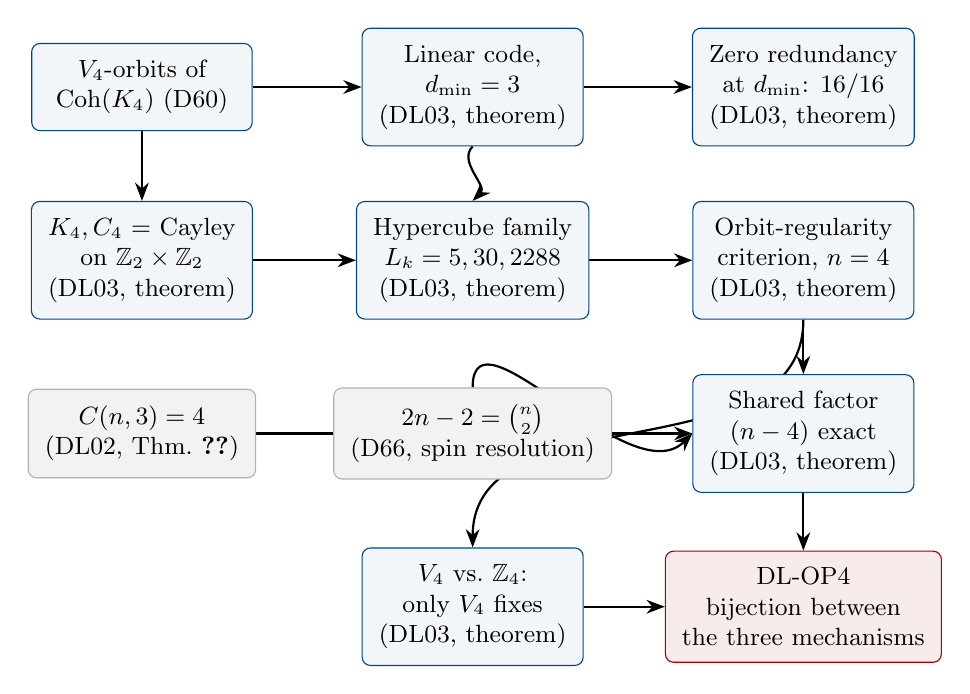
\begin{tikzpicture}[
  every node/.style={font=\small},
  theorem/.style={draw=proofblue, fill=proofblue!5,
    rounded corners=3pt, align=center, inner sep=6pt,
    minimum width=2.8cm, minimum height=0.9cm},
  conjecture/.style={draw=conjecturegreen, fill=conjecturegreen!8,
    rounded corners=3pt, align=center, inner sep=6pt,
    minimum width=2.8cm, minimum height=0.9cm},
  open/.style={draw=openproblemred, fill=openproblemred!8,
    rounded corners=3pt, align=center, inner sep=6pt,
    minimum width=2.8cm, minimum height=0.9cm},
  neg/.style={draw=orange!70, fill=orange!8,
    rounded corners=3pt, align=center, inner sep=4pt,
    minimum width=2.4cm, minimum height=0.7cm},
  ext/.style={draw=gray!60, fill=gray!10,
    rounded corners=3pt, align=center, inner sep=6pt,
    minimum width=2.8cm, minimum height=0.9cm},
  arr/.style={-Stealth, thick},
]

\node[theorem]  at ( 0.0,  0.0) (V4orbits) {$V_4$-orbits of\\$\mathrm{Coh}(K_4)$ (D60)};
\node[theorem]  at ( 4.2,  0.0) (linear)   {Linear code,\\$d_{\min}=3$\\(DL03, theorem)};
\node[theorem]  at ( 8.4,  0.0) (phonemic) {Zero redundancy\\at $d_{\min}$: 16/16\\(DL03, theorem)};

\node[theorem]  at ( 0.0, -2.2) (cayley)   {$K_4,C_4$ = Cayley\\on $\mathbb{Z}_2\times\mathbb{Z}_2$\\(DL03, theorem)};
\node[theorem]  at ( 4.2, -2.2) (hypercube) {Hypercube family\\$L_k=5,30,2288$\\(DL03, theorem)};
\node[theorem]  at ( 8.4, -2.2) (orbitcrit) {Orbit-regularity\\criterion, $n=4$\\(DL03, theorem)};

\node[ext]      at ( 0.0, -4.4) (dl02)     {$C(n,3)=4$\\(DL02, Thm.~\ref{thm:DL02_unique})};
\node[ext]      at ( 4.2, -4.4) (d66)      {$2n-2=\binom n2$\\(D66, spin resolution)};
\node[theorem]  at ( 8.4, -4.4) (factor)   {Shared factor\\$(n-4)$ exact\\(DL03, theorem)};

\node[theorem]  at ( 4.2, -6.6) (v4z4)     {$V_4$ vs.\ $\mathbb{Z}_4$:\\only $V_4$ fixes\\(DL03, theorem)};
\node[open]     at ( 8.4, -6.6) (DLOP4)    {DL-OP4\\bijection between\\the three mechanisms};

\begin{pgfonlayer}{background}
\draw[arr] (V4orbits.east)  -- (linear.west);
\draw[arr] (linear.east)    -- (phonemic.west);
\draw[arr] (V4orbits.south) -- (cayley.north);
\draw[arr] (cayley.east)    -- (hypercube.west);
\draw[arr] (linear.south) to[out=-135,in=45] (hypercube.north);
\draw[arr] (hypercube.east) -- (orbitcrit.west);
\draw[arr] (orbitcrit.south) -- (factor.north);
\draw[arr] (dl02.east)      -- (factor.west);
\draw[arr] (d66.north)      to[out=90,in=-135] (factor.west);
\draw[arr] (orbitcrit.south) to[out=-90,in=90] (v4z4.north);
\draw[arr] (factor.south)   -- (DLOP4.north);
\draw[arr] (v4z4.east)      -- (DLOP4.west);
\end{pgfonlayer}
\end{tikzpicture}%
}
\caption{The electron alphabet as an error-correcting code and the threefold characterisation of $n=4$: DL03 dependency chain (new in v33). \textcolor{proofblue}{Blue}: unconditional theorems. Grey: results recalled from D60, DL02, and D66 respectively, not re-derived. \textcolor{openproblemred}{Red}: open problem. The programme moves from the $V_4$-orbit structure of $\mathrm{Coh}(K_4)$ already established in D60, through the linear-code and zero-redundancy theorems and the Cayley--hypercube growth law, to a new orbit-regularity criterion for $n=4$ which, combined with DL02's triangle-count theorem and D66's spin-resolution theorem, is shown to share the exact algebraic factor $(n-4)$. The $V_4$-versus-$\mathbb{Z}_4$ result refines the mechanism further; DL-OP4 (whether the three mechanisms are one constraint or three coincidences) is the single open problem of this section.}
\label{fig:dependency_DL03}
\end{figure}

\newpage

% ============================================================
\section{Falsifiable Predictions}
\label{sec:predictions}

\begin{longtable}{L{0.5cm}L{3.2cm}L{5.2cm}L{4.2cm}}
\caption{Complete list of falsifiable, parameter-free PDL predictions (v31). All predictions follow from the quintuplet and $\Delta m_{\mathrm{iso}}$ alone, with no additional free parameters. Predictions P1--P6 are derived from the analytical chain; P7--P8 follow from Conjecture~$H_B$ (D41); P9 is derived from D45; P10 from D55; P11--P17 from D62 and D63; P18--P19 from D45~v2 and D65 (v30). D66 (v31) introduces no new numerical falsifiable prediction: its two theorems are structural (parity resolution, uniqueness of $n=4$), and its candidate physical interpretations (OP-D66pub-1, OP-D66pub-2) are explicitly flagged as open rather than asserted.}
\label{tab:predictions}\\
\toprule
\textbf{ID} & \textbf{Observable} & \textbf{PDL prediction} & \textbf{Test / status}\\
\midrule
\endfirsthead
\toprule
\textbf{ID} & \textbf{Observable} & \textbf{PDL prediction} & \textbf{Test / status}\\
\midrule
\endhead
\bottomrule
\endfoot
P1 & Proton--electron mass ratio $\mu$ & $\mu=1836.152\,670$ (parameter-free) & Testable at $0.001$~ppm; current CODATA: $1836.152\,673\,43(11)$; residual $1.8\times10^{-9}$.\\[0.4em]
P2 & Fine-structure constant $\alpha$ & $\alpha^{-1}=137.035\,999$ from quintuplet alone & Testable at $10^{-9}$; current agreement $\mathcal{O}(10^{-4})$; OP3/OP7 for residual.\\[0.4em]
P3 & Hubble constant ratio & $H_{0,\mathrm{local}}/H_{0,\mathrm{CMB}}=\sigma(N_{\mathrm{local}})/\sigma(40)$ & PDL prediction $1.085935$ vs.\ observed $1.0859\pm0.007$; $0.006\%$ error; zero free parameters.\\[0.4em]
P4 & CMB-epoch BH entropy suppression & Factor $\sigma(40)\approx 0.848$ relative to local universe & No direct observation yet; accessible via future CMB-$S_4$ constraints.\\[0.4em]
P5 & PBH survival threshold & $M^*_{\mathrm{PDL}}=\sigma(40)^{-2/3}\,M^*_{\mathrm{GR}}\approx 5.706\times10^{14}$\,g ($+11.89\%$) & Testable via Fermi-LAT IGRB analysis with \textsc{BlackHawk}/\textsc{Isatis}~\cite{D45}; excess Hawking flux at $\sim93$--$104$\,MeV.\\[0.4em]
P6 & AGN entropy-to-energy ratio & $S/E\propto G(N(z))$: systematic redshift trend & Traceable in cosmic-noon AGN surveys (JWST, Euclid); no contradicting data.\\[0.4em]
P7 & $B(E2)$ ratio in $^{90}$Ru/$^{88}$Ru & $R\approx 2.02$ (from $H_B$, $k=8\to10$) & Testable at FRIB or RIKEN; $^{88}$Ru beam available.\\[0.4em]
P8 & $N_{\mathrm{comp}}$ ratio $^{94}$Pd/$^{92}$Pd & $N_{\mathrm{comp}}(^{94}\mathrm{Pd})/N_{\mathrm{comp}}(^{92}\mathrm{Pd})=2.000\pm0.05$ & Testable from DNO-SM calculations with $^{94}$Pd spectroscopy at RIKEN.\\[0.4em]
P9 & IGRB spectral cutoff position & $E_c^{\mathrm{PDL}} \approx 93$\,MeV vs.\ $E_c^{\mathrm{GR}} \approx 104$\,MeV (shift $-10.6\%$) & Testable with Fermi-LAT IGRB data + \textsc{BlackHawk}/\textsc{Isatis}; requires non-zero $f_{\mathrm{PBH}}$ in $[5.10,\,5.71]\times10^{14}$\,g.\\[0.4em]
P10 & Isospin mass splitting $\Delta m_{\mathrm{iso}}$ & $\Delta m_{\mathrm{iso}} = 2.446$~MeV (from D55 C1+C3 formula, no free parameter) & FLAG 2024: $2.52 \pm 0.08$~MeV; compatible at $0.92\,\sigma$. Distinguishable from D30 value ($2.532$~MeV) at $\pm 0.04$~MeV precision (next-generation lattice QCD, 3--5 year horizon).\\[0.4em]
P11 & Electroweak vev $v$ & $v = 14161/54\cdot m_p = 246.20$~GeV (Conjecture~T1, D62) & PDG: $246.22$~GeV; deviation 676\,ppm. Entry point: OP-D62-1 for the correction to 41\,ppm.\\[0.4em]
P12 & $Z^0$ boson mass & $M_Z = 91.168$~GeV via analytical chain $\Delta\alpha(M_Z)$ (D62) & PDG: $91.1876$~GeV; tension $3.67\,\sigma$; traced to absence of hadronic corrections (OP-D62-4).\\[0.4em]
P13 & Higgs boson mass & $M_H/m_p = 133.611$, i.e.\ $M_H = 125.33$~GeV (D62) & PDG: $125.20 \pm 0.11$~GeV; tension $1.49\,\sigma$.\\[0.4em]
P14 & Valence quark mass ratio & $m_d/m_u = 2401/1104 \approx 2.1748$ (H\_mass, D63) & PDG: $2.162 \pm 0.063$; deviation $0.59\%$; no free parameter beyond $\Delta m_{\mathrm{iso}}$.\\[0.4em]
P15 & Up and down quark masses & $m_u = 2.155$~MeV, $m_d = 4.687$~MeV (H\_mass + D31, D63) & PDG: $2.16 \pm 0.07$~MeV, $4.67 \pm 0.15$~MeV; deviations $0.22\%$ and $0.37\%$.\\[0.4em]
P16 & Strange quark mass & $m_s = 93.08$~MeV (H\_sea, $n_s=52$, D63) & PDG: $93.5 \pm 0.8$~MeV; deviation $0.45\%$.\\[0.4em]
P17 & Charm, bottom, top quark masses & $m_c = 1301$~MeV ($n_c=92$), $m_b = 4081$~MeV ($n_b=120$), $m_t = 176169$~MeV ($n_t=332$) (H\_sea, D63) & PDG: $1270 \pm 30$, $4180 \pm 30$, $172760 \pm 720$~MeV; deviations $2.46\%$, $2.37\%$, $1.97\%$; top non-hadronisation structural ($r(332) \gg R_{\mathrm{sea}}$).\\[0.4em]
P18 & PBH photon spectral peak & $E_{\mathrm{peak}}=117.5$~MeV (PDL) vs.\ $130.1$~MeV (GR), $-9.65\%$ shift (D45~v2, \textsc{GammaPBHPlotter}/\textsc{BlackHawk}) & Independent spectral signature alongside the $+11.89\%$ mass-threshold shift (P5); testable with existing Fermi-LAT IGRB data.\\[0.4em]
P19 & Compact-object mass gap & Nucleon-dissolution threshold $M^*\approx4.3\,M_\odot$ (Conjecture, D65), from $\Zsat=20$ (D22) alone & Falls inside the observed lower mass gap; not tuned to do so. Sensitivity scan: $M^*\in[2.5,5.0]\,M_\odot$ for nuclear force range $r_c\in[1.39,2.21]$~fm, overlapping the pion Compton wavelength.\\[0.4em]
P20 & Engaged fraction of valence relations & $P_1=\Rsurf/\rval \to \varphi/3 = 0.539345$ as the closure size grows, under the D29 coupling criterion. & \textcolor{openproblemred}{Not yet computed} (OP-H$\varphi$-4). \textbf{This is a test of H$\varphi$ itself}: a limit differing from $\varphi/3$ refutes it, and with it the unconditional status of $\kappa$, $\alpha$ and Gate~3. Because $\Rsurf$ is an expectation, the target is a limit, not an exact equality.\\[0.3em]
\end{longtable}

% ============================================================
\section{Continuation Guide}
\label{sec:continuation}

\subsection{Entry points}
\label{subsec:entrypoints}
The following entry points are recommended for a colleague wishing to contribute to specific open problems.

\textcolor{negativered}{\textbf{Priority order, revised in v34.}} Two problems now sit \emph{directly on the causal chain to $G$} and take precedence over everything below: OP-B (the filter factor, reopened by D44v2) and OP-H$\varphi$-1 (the derivation of the self-similarity condition). Until one of them is closed, the chain C1--C4 $\to G$ is conditional. A third, OP-H$\varphi$-4, is the only identified route to \emph{refuting} H$\varphi$, and a negative result there is as valuable as a proof.

\begin{itemize}
\item \textbf{OP-B (filter factor $k$; reopened in v34):} Start from D44v2, which locates the arithmetic error and shows that both of D44~v1's constructions fail. The $S_4$-equivariance constraints of D42 remain available and are unaffected. Before attempting a new construction, verify against D44v2 that the failure mode is understood: compensating errors must be identified before corrections are applied.
\item \textbf{OP-H$\varphi$-1 (derive the self-similarity condition; new in v34):} The strongest available constraint is negative and should be used to prune the search: \emph{no counting rule can work}, because enumeration over a finite ensemble yields a rational and $\varphi/3$ is irrational. The condition must be a fixed point in which the engagement rate depends on the engagement already realised. C3 is an axiom of self-referential closure and is the natural place to begin. Do not look for five-fold symmetry: Section~\ref{subsec:phinegative} shows there is none in the derivation chain.
\item \textbf{OP-H$\varphi$-4 (falsification test; new in v34):} Immediately actionable. Compute the engaged fraction on proton analogues of increasing size under the D29 coupling criterion and test convergence to $\varphi/3$. Because $\Rsurf$ is an expectation and not a cardinality, the target is a limit, not an exact equality. \textbf{A negative outcome refutes H$\varphi$ and must be published as such.}
\item \textbf{OP-D68-7 (pulsation definitions; new in v34):} Blocking. Settle the divergence between D46's $\Phi$ and D68's $\sigma_S$ before any further use of D50 or D64 that relies on a uniform $P_2/P_1=-1$.
\item \textbf{OP1-D35 (leak constant $C$):} The most significant remaining foundational problem. Requires familiarity with D48 (coherence tensor), D17 (exponent~18 derivation), and D30 ($\eta_L$ structural factor). The question is whether the prefactor $C$ in $C^{(\mathrm{leak})}$ can be expressed as a closed-form function of the quintuplet, in the spirit of OP-B (resolved in D44).
\item \textbf{OP2 (global uniqueness):} Requires familiarity with D16, D16b, and combinatorial optimisation over integer lattices. The Colab infrastructure of D43 can be used to extend the computational search radius.
\item \textbf{OP7 (47~ppm residual in $\mu$):} Immediately actionable using the D43 Colab infrastructure. Start with the Group~I filters in D43, identify the residual at each stage, and test candidate combinatorial factors from C1--C4.
\item \textbf{OP12 (BH coefficient $\tfrac{1}{4}$):} \textcolor{proofblue}{Resolved by D50.} The coefficient $\tfrac{1}{4}$ in $\SBH = k_B A/(4\ell_P^2)$ is the stable fraction $4/16$ per surface relation (D29), with independence guaranteed by H3 (D42). $\Omega_{\mathrm{surf}} = 4^{\Rsurf}$, $S_{\mathrm{surf}} = k_B\Rsurf\ln 4$. Black hole thermodynamics layer complete.
\item \textbf{OP-London (London equation from PDL):} \textcolor{proofblue}{Resolved by D49.} See corpus table entry above.
\item \textbf{OP1-D35 (leak constant $C$):} \textcolor{proofblue}{Resolved by D51+D52.} See corpus table entry and Section~\ref{sec:openproblems} above.
\item \textbf{OP-D64-1 (macroscopic microstate counting; new in v30):} The single highest-priority entry point in the programme. Requires constructing a $K_4\leftrightarrow K_4$ coupling rule generalising the single-partner $(A)\wedge(B)$ criterion of D29 to macroscopic multiplicity. Start from the negative result of D64 (Proposition~\ref{prop:D64negative}) and the surface-restricted refinement, understanding precisely why the latter fails to generalise from one solar mass to M87*.
\item \textbf{OP-D65-3 (inhomogeneous, symmetry-broken regime; new in v30):} Requires extending the coherence stress-energy tensor (D48v3) and equation of state (D54) beyond the homogeneous limit $L\to\infty$. Identified in D65 as the common structural cause of three independent negative results; resolving it would remove the single largest obstacle to a quantitative black hole physics programme.
\item \textbf{OP-D66pub-3 (orientation-dependent nucleon observable; new in v31):} Requires an internally derived (not externally imported) spin-type magnitude for the nucleon. Every construction in D66 and D67 using the true physical spin magnitude ($1/2$) fails in principle; the open question is whether any internally derived magnitude could succeed. Highest priority of the D66/D67 open problems.
\item \textbf{OP-D67-1 (isolated nucleon in the inhomogeneous regime; new in v31):} Requires attempting a direct microstate count (D37/BH-1 style) for the bound, isolated nucleon, rather than the canonical-ensemble or ad hoc geometric routes already shown negative twelve times over (D66, D67).
\item \textbf{OP-OFN-2 ($\tau=90$ structural echo; new in v31):} Requires familiarity with the Matrix Tree Theorem computation of D66/N02 (Section~\ref{sec:PDLOFN}(vi)) and the independent theorems $\beta_1(K_4)=3$ (D23v2) and $\dim\mathcal P(1,3)=10$ (D35/D61). The question is whether a single combinatorial construction produces $\tau=90$ as $9\times10$ directly, rather than as a numerical coincidence of two separately-derived integers.
\end{itemize}

\subsection{Recommended next documents}
\label{subsec:nextdocs}
Given the current state of the programme, the following documents would have the highest impact:

\begin{enumerate}
\item \textbf{DM v31}: The present document. Incorporates D66 (search for a nucleon metric, parity-obstruction theorem and its spin resolution, second characterisation of $K_4$) and D67 (coplanarity theorem closing the D66 vector-construction route, corrected wave-closure relation, non-robust $18=2\times9$ lead), and records the completed, deposited Note~N02 (Section~\ref{sec:PDLOFN}), including the $G_E$/$G_H$ distinction, the $\tau=90$ invariant, and the CP-pair classification.
\item \textbf{D67 Zenodo deposit}: Reserve a DOI and deposit D67, verifying no collision with existing corpus numbering; update this document and \texttt{10.5281zenodo.txt} accordingly. Immediately actionable.
\item \textbf{The $K_4\leftrightarrow K_4$ coupling rule (OP-D64-1)}: The central missing structural ingredient blocking OP-D64-1, OP-D65-3, and the quark--gluon plasma regime near black hole formation. Highest priority of the entire programme at present.
\item \textbf{D-Kerr-extension}: Apply the D65 closure results (two coherence defects, curvature-migration exponent) systematically to the GW250114 reference target ($M_f=62.7\,M_\odot$, $\chi_f=0.68$), extending beyond the order-of-magnitude ringdown estimate of Section~\ref{subsec:GW250114}.
\item \textbf{OP-D66pub-3 --- an internally derived nucleon spin observable}: The highest-priority open problem introduced by D66; see Section~\ref{subsec:entrypoints} above.
\item \textbf{OP-D63-1 --- Formal independence in $\mathcal{Q}(K_n)$}: Resolution would elevate H\_mass to an unconditional theorem. \textbf{Entry point:} D47, D59, D63.
\item \textbf{OP-D62-4 --- Hadronic corrections to $M_Z$}: D63 provides $m_s \approx 93.1$~MeV as the necessary input. Entry point: D62, D63.
\item \textbf{OP-D61-2 / OP-OFN-1 --- Three fermion generations}: Formalise the link between $\beta_1(K_4) = 3$, $A_4/V_4 \cong \mathbb{Z}_3$, orbit $\mathcal{O}_5$, and three dynamical generation replicas. \textbf{Entry point:} N01, N02, D57, D59, D61, Section~\ref{sec:PDLOFN}.
\item \textbf{D-electroweak-WZ}: Derivation of the $W/Z$ mass ratio $M_W/M_Z = \cos(19\pi/119)$ as a parameter-free prediction. \textbf{Entry point:} D55, D57, D61.
\item \textbf{Experimental confrontations}: (i)~FLAG/lattice QCD for $\Delta m_{\mathrm{iso}}$ at $\pm 0.04$~MeV (D55, P10). (ii)~D45/D45~v2 predictions to \textsc{BlackHawk}/\textsc{Isatis} community, Fermi-LAT IGRB 50--200\,MeV window (mass threshold and spectral-peak shift). (iii)~Arbey/Auffinger (\textsc{BlackHawk}/\textsc{Isatis}) and Recchia/Lenzi (nuclear spectroscopy, D47 predictions at FRIB/RIKEN) outreach follow-up.
\item \textbf{D-nuclear-Z>82}: Extension of the valley-of-stability theorem to $Z>82$ (OP15).
\item \textbf{DL03}: Numerical enclosure of $n^*_{\mathrm{life}}$ from the gain function $R^1_{\mathrm{active}}$.
\end{enumerate}

% ============================================================
\section{Glossary}
\label{sec:glossary}

\begin{description}[leftmargin=3.5cm, style=nextline]
\item[AB criterion] The two-part stability criterion (amplitude condition A + balance condition B) that selects admissible two-closure couplings; proved exhaustively in D29 over $768$ configurations.
\item[Active surface $\Rsurf$] The set of valence coherence relations of the proton, $|\Rsurf|=\sigma=930$; the locus of all physical information exchange.
\item[Admissible closure] A finite signed graph satisfying all four axioms C1--C4; the minimal example is $K_4$.
\item[Born Level~1 / Level~2] Level~1 (D34, Theorem): modulus rule $P=|\psi|^2$ proved via Gleason uniqueness. Level~2 (D46, Theorem, OP4 resolved): $\mathrm{U}(1)$ phase freedom derived from $K_4$ sign equivalence and Hopf fibration structure.
\item[$\Ccoh$] Coherence stress-energy tensor appearing in the PDL Einstein equation; explicit form derived in D48v3, D51, D52: $C^{(\mathrm{mass})}$, $C^{(\mathrm{orb})}$, $C^{(\mathrm{spin})}$, and $C^{(\mathrm{leak})}$ all unconditional theorems. $C^{(\mathrm{spin})}=0$ in the ground state (OP-spin resolved, D48v3). All components in uniform units J\,m$^{-3}$. OP2-D35, OP1-D35, and OP-spin fully resolved. 
\item[Behaviour-versus-magnitude principle] The methodological claim, new in v30, that at the black hole scale PDL currently supports claims about topologically forced configurations, required functional forms, and threshold conditions (\emph{behaviour}), but not yet absolute entropy values or coupling strengths (\emph{magnitude}); proposed as a structural property of the theory's present domain of validity, not a temporary gap (D65).
\item[Coherence defect] A point of the internal state space $\mathcal{H}_{\mathrm{cyc}}$ where the coherent pulsation structure of $\Kfour$ cannot extend continuously over a closed surface; exactly two are forced on any closed spherical PDL surface, never zero, by a combinatorial analogue of the Poincar\'e--Hopf theorem (D65, Theorem~\ref{thm:2defects}).
\item[Parity obstruction] The impossibility of satisfying the classical $(A)\wedge(B)$ criterion jointly on both half-cycles of the $K_4$ pulsation with classical cross signs (zero joint solutions, D66, Theorem~\ref{thm:parityobstruction}); resolved by inserting a spin-type structure on the second half-cycle (D66, Theorem~\ref{thm:spinresolution}), whose operators coincide with the $\gamma^0,\gamma^i$ of D33.
\item[Coplanarity theorem] The result (D67, Theorem~\ref{thm:coplanarity}) that the electron reference direction and the D66 real-axis vectors of any mirror-symmetric nucleon pair are coplanar identically, with trivial $SU(2)$ holonomy; closes the D66 vector-construction route to a curvature-based nucleon metric without resolving OP-D64-3 itself.
\item[$G_E$, $G_H$] The two distinct graph structures carried by the OFN vacuum manifold $\Omega_{21}$, formally distinguished during the N02 integration (Session~72): $G_E$ is the dodecahedral graph (30 edges, 3-regular, spectral gap $\gamma_E=3-\sqrt5$); $G_H$ is the Hamming-distance-1 graph (22 edges, irregular, spectral gap $\lambda_1\approx0.0804$). The identity $\varphi+\gamma_E/2=2$ holds for $G_E$ only.
\item[$\tau$ (spanning-tree invariant)] $\tau=90$: the exact number of spanning trees of the connected 20-vertex component of $G_H$, derived via Kirchhoff's Matrix Tree Theorem (N02). Structural echo $\tau=b_1(K_4)^2\times\dim\mathcal P(1,3)=9\times10$, status open (OP-OFN-2).
\item[Curvature-migration exponent] The exponent governing how the polar curvature deficit of a PDL closure migrates towards the equator as the spin parameter $\chi$ approaches extremality; equal to exactly $1$ in arbitrary-precision arithmetic (D65), an open tension with the third law of black hole thermodynamics (OP-D65-2).
\item[Dissolution threshold $M^*$] The critical mass $M^*\approx4.3\,M_\odot$ at which the density required for nucleon dissolution (from $\Zsat=20$, D22, and the nuclear force range) coincides with the Schwarzschild condition; falls inside the observed compact-object mass gap without tuning (D65, Conjecture~\ref{conj:dissolution}).
\item[$K_4\leftrightarrow K_4$ coupling rule] The identified but not yet constructed axiomatic prescription for how two or more engaged $\Kfour$-closures jointly contribute degrees of freedom at macroscopic multiplicity, generalising the single-partner $(A)\wedge(B)$ criterion of D29; the single highest-priority missing structural ingredient for OP-D64-1 (macroscopic microstate counting).
\item[Soft-hair correspondence] The structural analogy, established in D64, between the PDL surface-degeneracy theorem $\Omega_{\mathrm{surf}}=4^{\Rsurf}$ (D50) and the Hawking--Perry--Strominger soft-hair programme; explicitly not a claim of mathematical identity.
\item[Coherence-pulsation cost] $|\mathcal{Q}(K_n)| = r(n)\cdot n^3 = n^4(n-1)/2$: the cardinal of the coherence-pulsation quadruplet set of a valence core $K_n$; governs the valence quark mass ratio via Conjecture H\_mass (D63).
\item[Conjecture H\_mass] $m_d/m_u = 2401/1104$: the ratio of coherence-pulsation costs of $K_{n_d}$ and $K_{n_u}$; identified by exhaustive scan of degree-$\leq 5$ monomials; no additional free parameter beyond $\Delta m_{\mathrm{iso}}$ (D63).
\item[Conjecture H\_sea] $m_{\mathrm{sea}}(n) = [n^4(n-1)/n_u^4(n_u-1)]\cdot[R_{\mathrm{sea}}/(R_{\mathrm{sea}}+r(n))]\cdot m_u$: effective mass of a pseudo-stationary sea quark regime; weighting $w(n)$ selected by exhaustive scan over 5 candidates (D63).
\item[Hadronisation boundary] $n_{\max} = 140$: maximum effective size (multiple of~4) such that $r(n) \leq R_{\mathrm{sea}}$; corresponding maximum effective mass $\approx 7677$~MeV; the top quark ($n_t = 332$, $r(332) \gg R_{\mathrm{sea}}$) lies above this boundary and cannot form hadrons (D63, structural corollary).
\item[Residual fluidity] $w(n) = R_{\mathrm{sea}}/(R_{\mathrm{sea}}+r(n))$: fraction of the extended relational budget $R_{\mathrm{sea}}+r(n)$ that remains available as fluid sea when a pseudo-stationary structure of size $n$ is present; governs Conjecture H\_sea (D63).
\item[Structural identity] $n_u - 1 = p_{k_1} = 23$: exact integer identity between two unconditional theorems of C1--C4 --- the valence up-quark size ($n_u = 24$, D47) and the first cosmological leakage prime ($p_{k_1} = p_9 = 23$, D51) --- connecting the hadronic and cosmological sectors for the first time (D63).
\item[Coherence cost] Fraction of violated triangles (negative-product edges) in a signed graph; minimised by axiom C4.
\item[DL series] Documents DL01, DL02, \ldots; the PDL-V programme extending C1--C4 to self-replication and complexity thresholds. Structurally separate from the D series; presented in Part~III of this document.
\item[$\delta^*$] Optimal lineage variation in the PDL-V programme; $\delta^* = 1/2$, equal to the half-pulsation of $K_4$; proved invariant under the rarity law (DL01).
\item[$\epsGeomB$] Geometric correction factor in the PDL mass-ratio formula; closed-form expression $\epsGeomB = \kappa \cdot C/(6+\kappa)\cdot(1+2/\Rtot) \in \mathbb{Q}(\sqrt{5})$ proved in D44 (OP8 resolved).
\item[Equation of state $w(N)$] The ratio $P/(\rhocoh c^2)$ for the PDL coherence fluid; $w(N) = -\rho_\Lambda/\rhocoh(N)$ (D54, unconditional theorem). At coherence densities $|w| \sim 10^{-44}$ (cold matter); at cosmological scales $\Omega_\Lambda^{\mathrm{PDL}} = 0.6838$ (dark energy, $0.17\%$ from Planck 2020).
\item[$f(n)$] Rarity law in the PDL-V programme; $f(n) = 2^{n+1-\binom{n}{2}}$, doubly exponentially decreasing; exponents are triangular numbers (DL01, exact theorem).
\item[$\Geff(N)$] Effective gravitational coupling at scale $N$; equal to $\sigmaN\cdot\GPDL$ by Gate~3 (unconditional theorem).
\item[Gate 1, 2, 3] Three critical proof milestones. Gate~1: $155/11017$ from axioms (D29). Gate~2: $a=2$ from axioms (D30). Gate~3: $\Geff=\sigmaN\cdot\GPDL$ (D36/D42, unconditional).
\item[H1, H2, H3] Named hypotheses of the programme. H1 ($\kappa=\Rsurf/\Rtot$): follows from H3 (D42) via D39, but is \textcolor{hypothesisorange}{conditional on H$\varphi$}, since $\Rsurf$ is a hypothesis. \textcolor{negativered}{Earlier versions of this glossary wrote H1 as $\kappa=\sigma/R_{\mathrm{tot}}$ with $\sigma=930$; that expression evaluates to $0.084415$, not $\kappa=0.045529$, and is incorrect.} H2 (bridge linearity): absorbed into D36. H3 (Indifference Lemma): proved unconditionally in D42.
\item[H$\varphi$] Named hypothesis, introduced in v34: $\Rsurf=\varphi\,\rval/3=310\varphi$. Not derived from C1--C4 (Section~\ref{sec:Hphi}). $\kappa$, $\alpha$, $\sigmaN$, $\Geff$, the Hubble prediction and $\Lambda$ are conditional on it. Introduces no adjustable parameter.
\item[$\rval$] Valence relational content, $\rval=2\binom{24}{2}+\binom{28}{2}=930$. \textcolor{negativered}{Earlier versions of this document called this quantity $\sigma$ and described it as ``the active surface''; it is neither the active surface nor to be confused with the engagement fraction $\sigmaN$.}
\item[$r_{\mathrm{core}}$] Mean coherence core per valence quark, $\rval/3=310$. The proton has three valence cores: $n_{u\text{-cores}}=2$, $n_{d\text{-cores}}=1$.
\item[$\Rsurf$] Active surface: the \emph{expected} number of valence relations engaged in coherent external coupling, $310\varphi\approx501.59$ under H$\varphi$. An expectation under the uniform measure of D42, \textbf{not a cardinality} --- an irrational cannot be the size of a set.
\item[$\Rres$] Residual valence content, $\rval-r_{\mathrm{core}}-\Rsurf=310/\varphi^2\approx118.409$. Defined by subtraction; \textbf{no relational interpretation exists in the corpus} (OP-H$\varphi$-3).
\item[$n_{\mathrm{sea}}$] Number of faces (equivalently, cells) of the quadrangulated sea. Never assigned a value in the corpus. The rule $\Rsea=2n_{\mathrm{sea}}$ holds for a \emph{closed} sea; with a boundary the identity is $E=2F+b/2$ (Section~\ref{sec:searule}).
\item[$b$] Total perimeter of the three holes of the sea, $b=204$. Formerly a simulation output ($2E-4F$); expressible as $2(n_K+(\Delta n+1)^2+1)$ under Conjecture~\ref{conj:mesh}.
\item[Hopf fibration] The fibre bundle $S^1\hookrightarrow S^3\to S^2$ generating the $\mathrm{U}(1)$ phase freedom of quantum mechanics; its appearance in D46 is a structural consequence of the $K_4$ pulsation sign equivalence.
\item[Indifference Lemma (H3)] The probability measure on the relations of a PDL closure is uniform; the unique measure compatible with $S_4$-symmetry of $K_4$. Proved from C1--C4 in D42 via three lemmas.
\item[$K_4$] The complete signed graph on four vertices and six edges; the unique minimal admissible closure (D16a theorem); identified with the electron prototype.
\item[$\kappa$] Primary leakage parameter; $\kappa=310\varphi/11017\in\mathbb{Q}(\sqrt{5})$; unconditional theorem of C1--C4 (D42 corollary); $\kappa\approx 0.0455$.
\item[Mirror Lemma] The proton and neutron HO-PDL levels are isomorphic, sharing the same splitting $s=1/12$, level order, and degeneracies (D47, Lemma~5.2, from D22-N2).
\item[$m_{\mathrm{iso}}$] Isospin mass splitting $m_d-m_u$; the unique irreducible external parameter of the programme (Gate~2, D30).
\item[$N_{\mathrm{CMB}}$] PDL-derived CMB epoch parameter; $N_{\mathrm{CMB}}=40$ from neutron quintuplet (D27 theorem).
\item[$n^*_{\mathrm{life}}$, $n^*_{\mathrm{consciousness}}$, $n^*_{\mathrm{max}}$] Life, consciousness, and maximum complexity thresholds in the PDL-V programme; existence and strict ordering proved (DL02); numerical values open (DL-OP1, DL-OP2).
\item[OP$n$] Open Problem $n$; see Section~\ref{sec:openproblems}. OP1, OP4, OP8, OP12, OP13, OP-London, OP1-D35, and OP-pressure fully resolved. OP14 reopened in v32 (D47v2); see Open Problem~\ref{op:filling}.
\item[PDL] Projective Dynamic Logo; the research programme initiated in D01.
\item[PDL-V programme] Extension of PDL to self-replication and complexity thresholds; inaugurated by DL01 and DL02; see Part~III.
\item[Quintuplet] The integer tuple $\quintuplet$ characterising the proton; $\nu_u=24$, $\nu_d=28$, $\sigma=930$, $R_{\mathrm{sea}}=10087$, $R_{\mathrm{tot}}=11017$.
\item[$\rhocoh(N)$] Coherence mass density at scale $N$; $\rhocoh = \sigmaN\cdot\Rsurf\cdot m_p/(V_C\cdot\Rtot)$ (D48v3 theorem).
\item[$S(\Gamma)$] Constraint-structure operator in the PDL-V programme; $S(K_4) \cong K_4$ (DL01 theorem).
\item[$\sigmaN(N)$] Coherence engagement fraction at scale $N$; $\sigmaN=1-(1-\kappa)^N\in\mathbb{Q}(\sqrt{5})$; $\sigmaN(40)\approx 0.8449$.
\item[$\Tpp$] Proton--proton conflict unit; $C(Z>20)=190\,\Tpp$ exactly (D40 theorem).
\item[$V_C$] Coherence volume; $V_C=(4/3)\pi[\hbar/(m_pc)]^3$; unconditional theorem of C1--C4 via D10a (temporal chain, Chain~1). D48v3 theorem.
\item[Valley of stability] Minimum neutron number $N_{\min}(Z)$ for stable nuclei; reproduced at $74$--$88\%$ accuracy for $Z=1$--82 by D40's original empirical filling-rate table under the corrected reconstruction formula (D47v2); \emph{not yet} an unconditional theorem of C1--C4 (OP14 reopened, Open Problem~\ref{op:filling}).
\item[18-filter hierarchy] The decomposition $18=6+5+4+3$ of the leakage exponent into four topological levels (D06, D17, D23).
\end{description}

% ============================================================
\newpage
\part{The PDL-V Programme: Life and Consciousness}
\label{part:PDL-V}
% ============================================================

\begin{center}
\textit{This Part is structurally separate from Parts I and II.\\
It presents a rigorous extension of the PDL framework to self-replication\\
and complexity thresholds, in a domain distinct from the physical constants programme.\\
The same axioms C1--C4 are used; the domain of application is different.}
\end{center}

\vspace{1em}

% ============================================================
\section{Introduction to the PDL-V Programme}
\label{sec:PDLV_intro}
% ============================================================

The PDL-V programme asks whether the axioms C1--C4, which determine the proton architecture and all derived physical constants, also constrain the structural conditions for self-replication and the emergence of biological and cognitive complexity. Documents DL01 and DL02 do not make biological claims; they establish mathematical threshold theorems that any system satisfying C1--C4 must obey. The connection to biology and consciousness is conjectural and is explicitly labelled as such.

\subsection{Separation from the physics programme}

The DL series shares the axiomatic foundation (C1--C4 and $K_4$) with the D series, but operates in a domain where the ``configurations'' are hierarchical graph structures rather than physical coherence cycles. The results of DL01 and DL02 are theorems of C1--C4 applied to this domain, with full epistemic rigour, but their physical interpretation involves a conjecture (the PDL-V Conjecture, DL01) that is not yet derivable from first principles. This conjecture is explicitly identified and is not presented as a theorem.

\subsection{Reading note}

A reader whose sole interest is the physical constants programme (gravitational constant, cosmological constant, nuclear structure, etc.) may skip Part~III without loss of continuity. A reader interested in the structural limits of self-replication and complexity should read DL01 first (operators $L$, $S$, $R^k$; rarity law; $\delta^*$ invariant), then DL02 (threshold hierarchy theorem).

% ============================================================
\section{Self-Replication Operators and the Rarity Law (DL01)}
\label{sec:DL01}
% ============================================================

\begin{theorem}[$K_4$ fixed point of $S$, \cite{DL01}]
\label{thm:DL01_fixedpoint}
Let $S(\Gamma)$ be the constraint-structure operator acting on admissible signed graphs. The complete graph $K_4$ is the unique fixed point of $S$: $S(K_4) \cong K_4$. This has been verified computationally over all 8 coherent configurations of $K_4$.
\end{theorem}

\begin{theorem}[Rarity law and $\delta^*$ invariant, \cite{DL01}]
\label{thm:DL01_rarity}
The fraction of self-replicating configurations at level $n$ satisfies the exact law:
\begin{equation}
f(n) = 2^{n+1-\binom{n}{2}},
\end{equation}
with exponents equal to $-T_{n-2}$ (triangular numbers): $f(n)$ is doubly exponentially decreasing. The optimal lineage variation $\delta^* = 1/2$ is an invariant equal to the half-pulsation of $K_4$; it is independent of $n$. The weak self-representation relation $R^1_{\mathrm{weak}}$ is forced at $100\%$ for all $n \geq 4$, verified for $n = 4$--$7$.
\end{theorem}

% ============================================================
\section{Threshold Hierarchy Theorems (DL02)}
\label{sec:DL02}
% ============================================================

\begin{theorem}[$K_4$ unique fixed point, \cite{DL02}]
\label{thm:DL02_unique}
$K_4$ is the unique fixed point of $S$ over all admissible closures. The equation $C(n,3) = n(n-1)(n-2)/6 = 4$ has $(n-1)(n-2) = 6$ as its only positive integer solution: $n = 4$. This is an unconditional theorem of C1--C4.
\end{theorem}

\begin{theorem}[Strict threshold separation, \cite{DL02}]
\label{thm:DL02_separation}
For $n \geq 5$, $|S^1(K_n)| \neq |S^2(K_n)|$: the first and second iteration of $S$ produce distinct orbit sizes. This forces a strict separation between the life threshold and the consciousness threshold: $n^*_{\mathrm{life}} < n^*_{\mathrm{consciousness}}$. This is an unconditional theorem of C1--C4.
\end{theorem}

\begin{theorem}[Finiteness of all thresholds, \cite{DL02}]
\label{thm:DL02_finiteness}
The doubly exponential rarity law $f(n) = 2^{n+1-\binom{n}{2}}$ implies that all thresholds $n^*$ are finite: $n^*_{\mathrm{max}} < \infty$. Combined with Theorems~\ref{thm:DL02_unique} and~\ref{thm:DL02_separation}, this gives the unconditional hierarchy:
\begin{equation}
4 \;<\; n^*_{\mathrm{life}} \;<\; n^*_{\mathrm{consciousness}} \;<\; n^*_{\mathrm{max}} \;<\; \infty.
\end{equation}
\end{theorem}

% ============================================================
\section{The Electron Alphabet as an Error-Correcting Code and a Threefold Characterisation of \texorpdfstring{$n=4$}{n=4} (DL03)}
\label{sec:DL03}
% ============================================================

DL03~\cite{DL03} (Session~74) reports three unconditional, computationally verified results obtained while probing what a combinatorial \emph{alphabet} carried by admissible closures would need to look like, as a candidate route towards giving the DL02 thresholds operational content. No numerical value for $n^*_{\mathrm{life}}$ or $n^*_{\mathrm{consciousness}}$ is established; the results below strengthen the structural context of Theorem~\ref{thm:DL02_unique} without superseding it.

\subsection{The electron alphabet is a maximum-distance linear code}

\begin{theorem}[Linearity and minimum distance, \cite{DL03}]
\label{thm:DL03_code}
Identify $\mathrm{Coh}(K_4)\subset\{\pm1\}^6$ with a binary code via $\pm1\leftrightarrow\{0,1\}$. Then $\mathrm{Coh}(K_4)$ is closed under coordinatewise multiplication (a subgroup of $\{\pm1\}^6$), with Hamming weight distribution $\{0,3,3,3,3,4,4,4\}$, hence minimum distance $d_{\min}=3$: a single-error-correcting code saturating the Hamming bound at length~6, eight codewords.
\end{theorem}

\begin{theorem}[Zero redundancy at minimal distance, \cite{DL03}]
\label{thm:DL03_phonemic}
Of the sixteen pairs of codewords in $\mathrm{Coh}(K_4)$ at Hamming distance $d_{\min}=3$, all sixteen lie in distinct $V_4$-orbits (verified exhaustively; zero exceptions). The same two properties (linearity, and $100\%$ orbit-change at $d_{\min}=3$) hold identically for $\mathrm{Coh}(Q_3)$ under $\mathbb{Z}_2^3$ (128 codewords, 512 minimal pairs, verified exhaustively), showing the result is not an artefact of $K_4$'s small size.
\end{theorem}

\subsection{The Cayley--hypercube family}

\begin{theorem}[\texorpdfstring{$K_4$}{K4} and \texorpdfstring{$C_4$}{C4} as Cayley graphs, \cite{DL03}]
\label{thm:DL03_cayley}
$K_4\cong\mathrm{Cay}(\mathbb{Z}_2\times\mathbb{Z}_2,S_{\mathrm{dense}})$ and $C_4\cong\mathrm{Cay}(\mathbb{Z}_2\times\mathbb{Z}_2,S_{\mathrm{sparse}})$, where $S_{\mathrm{dense}}$ is the set of all three non-zero elements and $S_{\mathrm{sparse}}$ the two unit-weight generators. $K_4$ and $C_4$ are the dense and sparse Cayley graphs on the same group, not unrelated small graphs.
\end{theorem}

Defining $L_k$ as the number of orbits of $\mathrm{Coh}(Q_k)$ under the coordinate-flip group $\mathbb{Z}_2^k$ for the hypercube $Q_k=\mathrm{Cay}(\mathbb{Z}_2^k,S_{\mathrm{sparse}})$, exhaustive enumeration gives $L_2=5$, $L_3=30$, $L_4=2288$ (orbit-size distribution $\{1{:}16,4{:}140,8{:}240,16{:}1892\}$ at $k=4$), a growth ratio itself accelerating ($6.0\to76.3$): the family diverges super-exponentially, embedding the electron's five-letter alphabet as the base case $k=2$.

\subsection{A threefold characterisation of \texorpdfstring{$n=4$}{n=4}}

\begin{theorem}[Orbit-regularity criterion, \cite{DL03}]
\label{thm:DL03_orbit}
$n=4$ is the unique value, among $n=2,\ldots,28$, for which $\mathrm{Coh}(K_n)$ possesses a non-trivial orbit under $S_n$ (via the bipartition parametrisation of Harary's theorem) of size exactly four --- the order required for a group to act regularly upon it (Lagrange). Verified exhaustively; no other $(n,k)$ pair in this range yields size four.
\end{theorem}

\begin{theorem}[Shared algebraic factor, \cite{DL03}]
\label{thm:DL03_factorisation}
The polynomials underlying Theorem~\ref{thm:DL02_unique} (DL02, $C(n,3)=4$) and D66's spin-resolution theorem ($2n-2=\binom n2$) share the linear factor $(n-4)$ exactly, verified by exact polynomial division:
\begin{equation}
n(n-1)(n-2)-24 = (n-4)(n^2+n+6), \qquad n(n-1)-2(2n-2) = (n-4)(n-1).
\end{equation}
The remaining factors differ in character: $n^2+n+6$ has no real root; $n-1$ has the real root $n=1$, excluded by D66's stated domain $n>1$. Theorem~\ref{thm:DL03_orbit} resolves to $(n-4)=0$ alone, with no residual factor. Whether the three mechanisms are three readings of one underlying constraint, rather than independent coincidences sharing a common root, is Open Problem~DL-OP4 (\ref{op:DL_bijection}).
\end{theorem}

\begin{theorem}[\texorpdfstring{$V_4$}{V4} versus \texorpdfstring{$\mathbb{Z}_4$}{Z4}, \cite{DL03}]
\label{thm:DL03_v4z4}
At $n=4$, $V_4$ acts regularly on the size-four orbit of Theorem~\ref{thm:DL03_orbit} and fixes the remaining four configurations pointwise (D60, Theorem~\ref{thm:K4}). The cyclic group $\mathbb{Z}_4\le S_4$ also acts regularly on the same orbit (Lagrange, order alone) but does \emph{not} fix the remainder pointwise (verified directly). Regularity is a fact about group order; pointwise fixing is specific to the Klein structure of $V_4$.
\end{theorem}

Figure~\ref{fig:dependency_DL03} summarises the complete dependency chain of this section.

\subsection{Open problems in the PDL-V programme}

\begin{openproblem}[DL-OP1 --- Numerical value of $n^*_{\mathrm{life}}$]
\label{op:DL_nlife}
The existence and strict ordering of $n^*_{\mathrm{life}}$ is established analytically (DL02). Its numerical value remains open. The gain function $R^1_{\mathrm{active}}(n)$ must be derived in closed form and its first zero located. \textbf{Priority:} high. \textbf{Entry point:} DL01, DL02.
\end{openproblem}

\begin{openproblem}[DL-OP2 --- Numerical value of $n^*_{\mathrm{consciousness}}$]
\label{op:DL_nconsciousness}
Analogous to DL-OP1 but for the second threshold. Requires DL-OP1 as a prerequisite. \textbf{Priority:} medium. \textbf{Entry point:} DL01, DL02.
\end{openproblem}

\begin{openproblem}[DL-OP3 --- Connection to physical substrate]
\label{op:DL_substrate}
The PDL-V conjecture (DL01) proposes that the threshold $n^*_{\mathrm{life}}$ corresponds to a specific physical structure derivable from C1--C4. This connection has not been derived and remains a conjecture. A formal derivation would require identifying the physical interpretation of the graph complexity level $n$ in terms of molecular or cellular organisation. \textbf{Priority:} exploratory. \textbf{Entry point:} DL01.
\end{openproblem}

\begin{openproblem}[DL-OP4 --- Bijection between the three characterisations of $n=4$]
\label{op:DL_bijection}
Construct an explicit bijection between the three independent mechanisms that single out $n=4$ (DL02's Theorem~\ref{thm:DL02_unique}, D66's spin-resolution theorem, and DL03's orbit-regularity criterion, Theorem~\ref{thm:DL03_orbit}), establishing that they are three readings of a single underlying constraint rather than three independent constructions sharing a common algebraic factor $(n-4)$ (Theorem~\ref{thm:DL03_factorisation}) by coincidence of the specific target values each was set up to solve for. \textbf{Priority:} medium. \textbf{Entry point:} DL02, D66, DL03.
\end{openproblem}

\clearpage

% ============================================================
\bibliographystyle{unsrturl}
\bibliography{PDL_Global_Mapping_v34_references}

\end{document}